\chapter{Scenarios}
\label{ch:scenarios}
% ##################################################################################################################

\hfill \textbf{Authors:} Andreas Horni, Marcel Rieser, Benjamin Kickhöfer, Dominik Ziemke, Joschka Bischoff, ...

\begin{center} 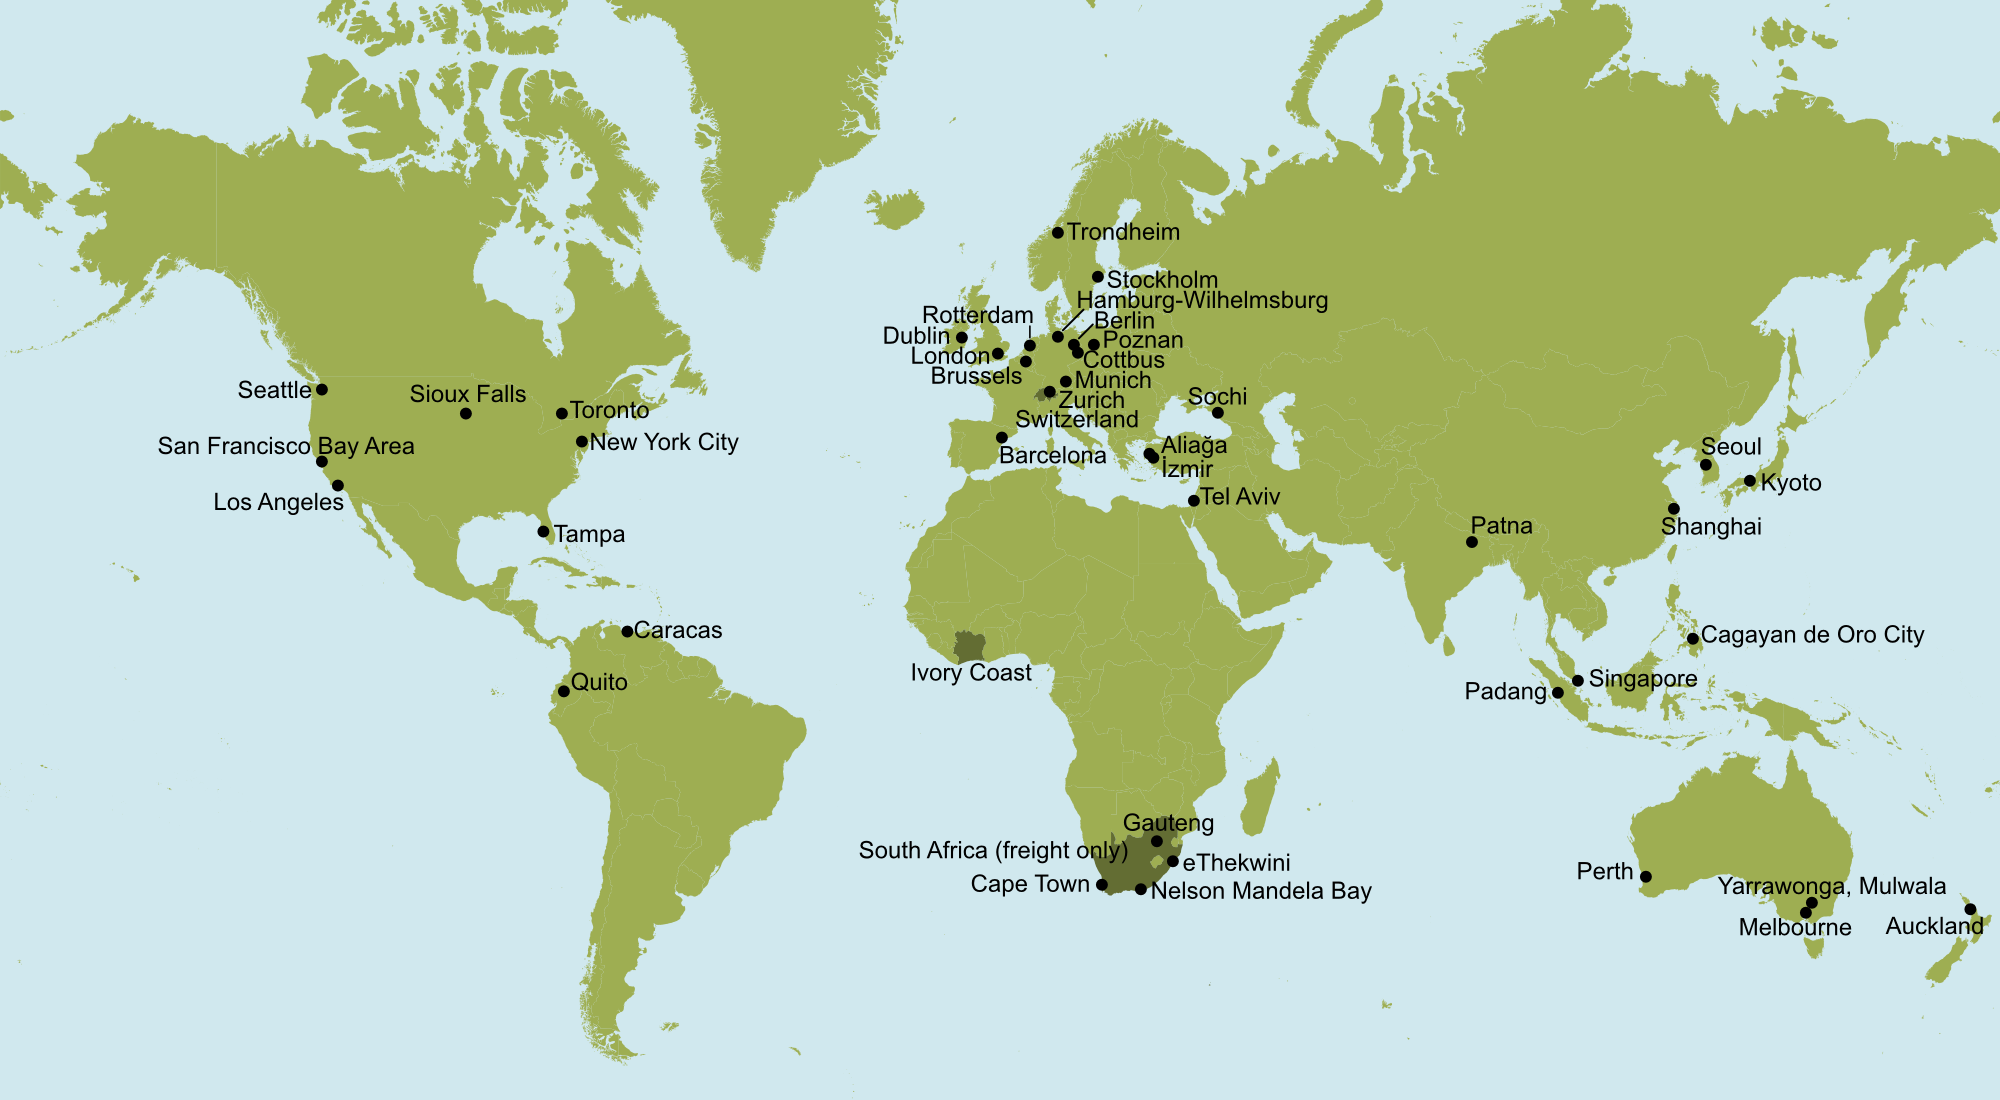
\includegraphics[width=0.7\textwidth, angle=0]{using/figures/MATSimModelsMap} \end{center}

% ##################################################################################################################
This chapter summarizes available MATSim scenarios as located on the map in Figure~\ref{fig:scenarios} and summarized at \citet[][]{MATSIM-T-Scenarios_Webpage_2014}).

Many scenarios are not public due to data privacy issues. However, knowing about the general methods and approaches adopted for scenario creation and hearing about problems faced thereby might significantly support the building of new scenarios. Content basically covers information on study area, population and demand generation, activity locations, network, simulated modes, calibration and validation, achieved results, associated projects, where to find more, where emphasis is put on specialties of a certain scenario, be it parsimonious data usage procedures, special modules used, or special modes simulated (such as the parataxis in the Gauteng scenario). Some of the scenarios are used since years with a continuous further development. We target at reporting, the latest version. 

Different levels of MATSim involvement are possible. For some regions and projects, MATSim is, for example, only used for traffic assignment whereas for others the complete demand is endogenously handled. Couplings with other forecasting models for transport demand generation have been successfully applied such as the coupling with TASHA for Toronto or the combination of MATSim with the activity-based transport model of Tel Aviv.

\createfigure%
{Scenarios Overview}%
{Scenarios Overview}%
{\label{fig:scenarios}}%
{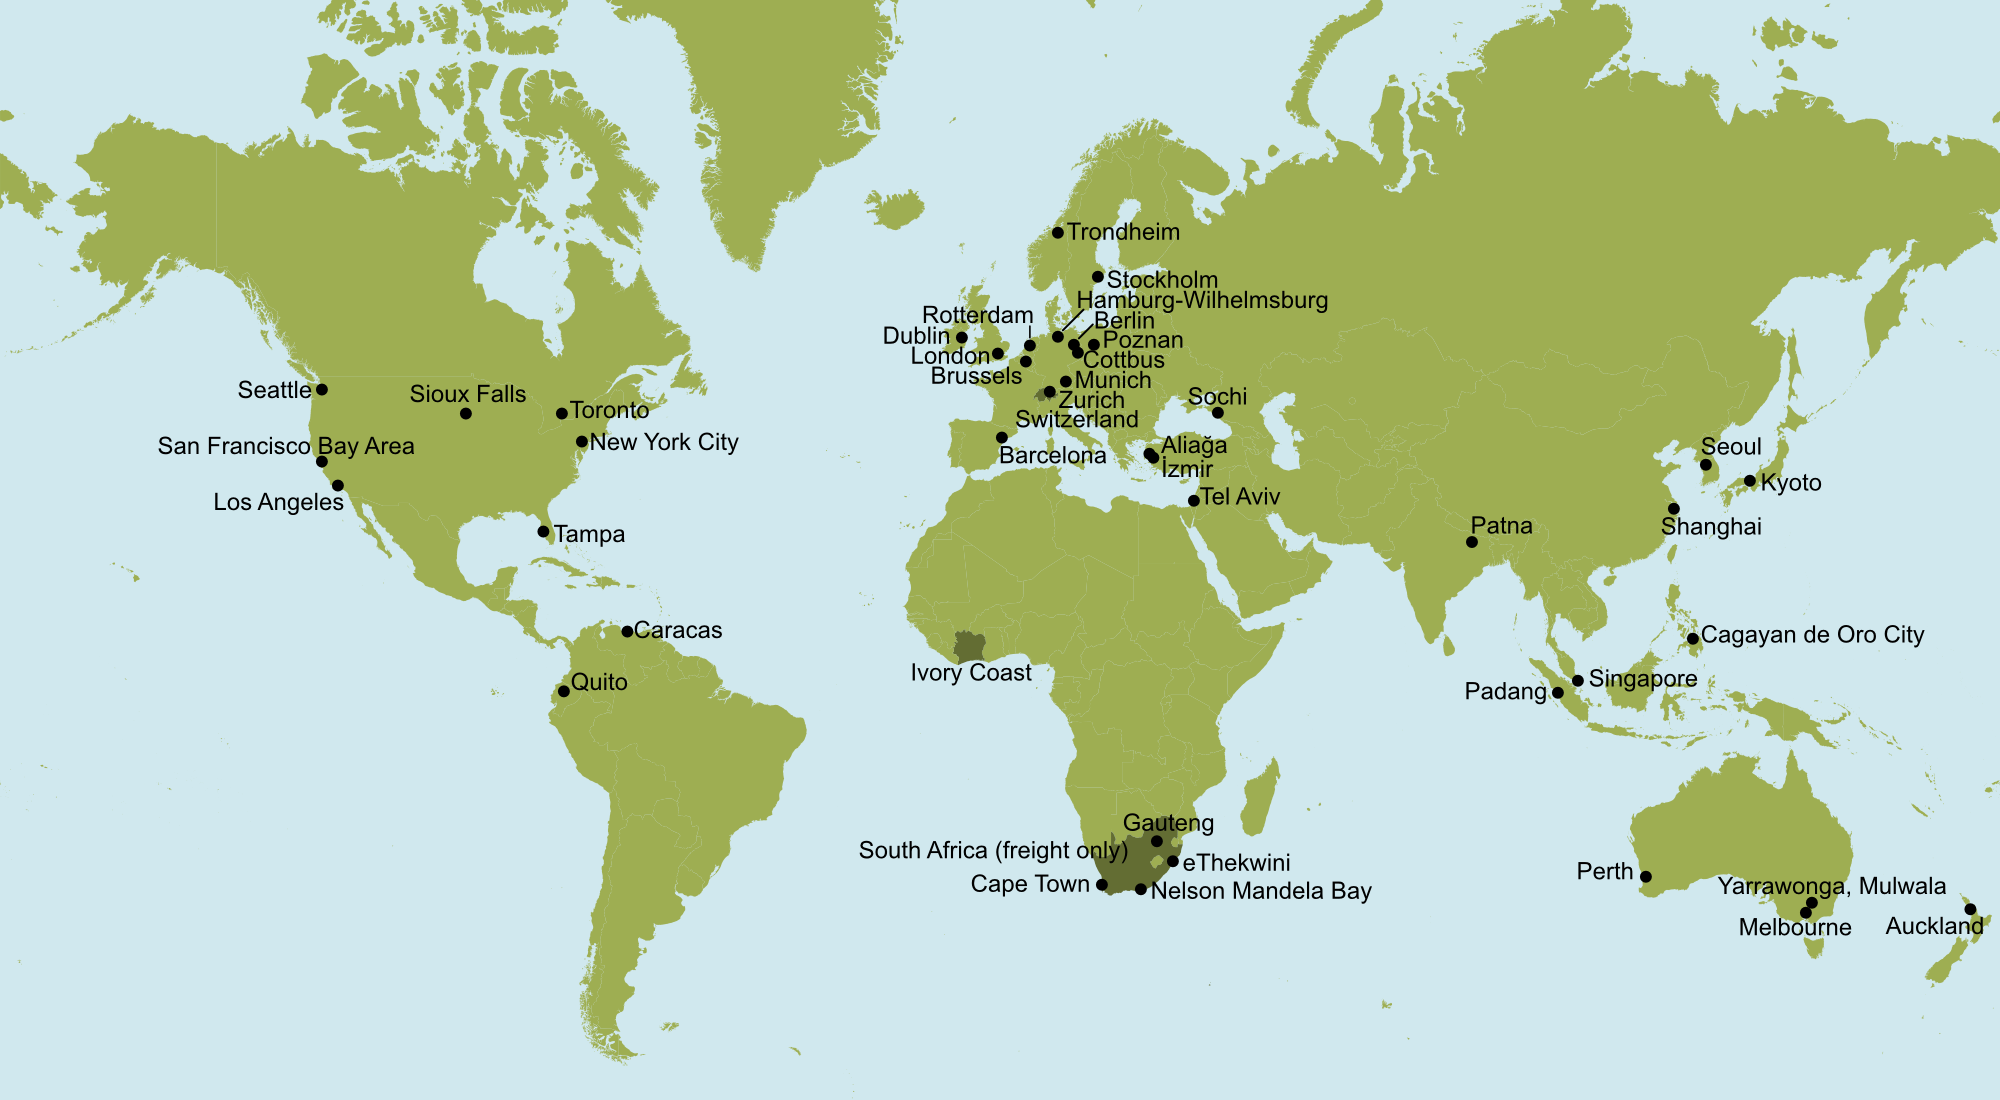
\includegraphics[width=0.99\textwidth, angle=0]{using/figures/MATSimModelsMap}}%
{}

% ==================================================================================================================
% ##################################################################################################################
\section{Berlin I: BVG Scenario}
\label{sec:berlinI}
\hfill \textbf{Author:} Andreas Neumann

% ##################################################################################################################
The \gls{bvg} is Berlin's main public transport company and runs all kind of services with the exception of the S-Bahn urban rail system. This includes bus services, the subway network, the largest tram network of Germany as well as ferry services. The bus network consists of 149\,different lines, 6\,468 directed stops and a vehicle fleet of 1\,316 buses \citep{BVG2012}. In total, about 937\,million trips were served by \gls{bvg} in 2012, 41\,\% of them by bus.

% ------------
\createfigure%
{The city of Berlin and its transit network.}%
{The city of Berlin and its transit network.}%
{\label{fig:scenario_berlin_i}}%
{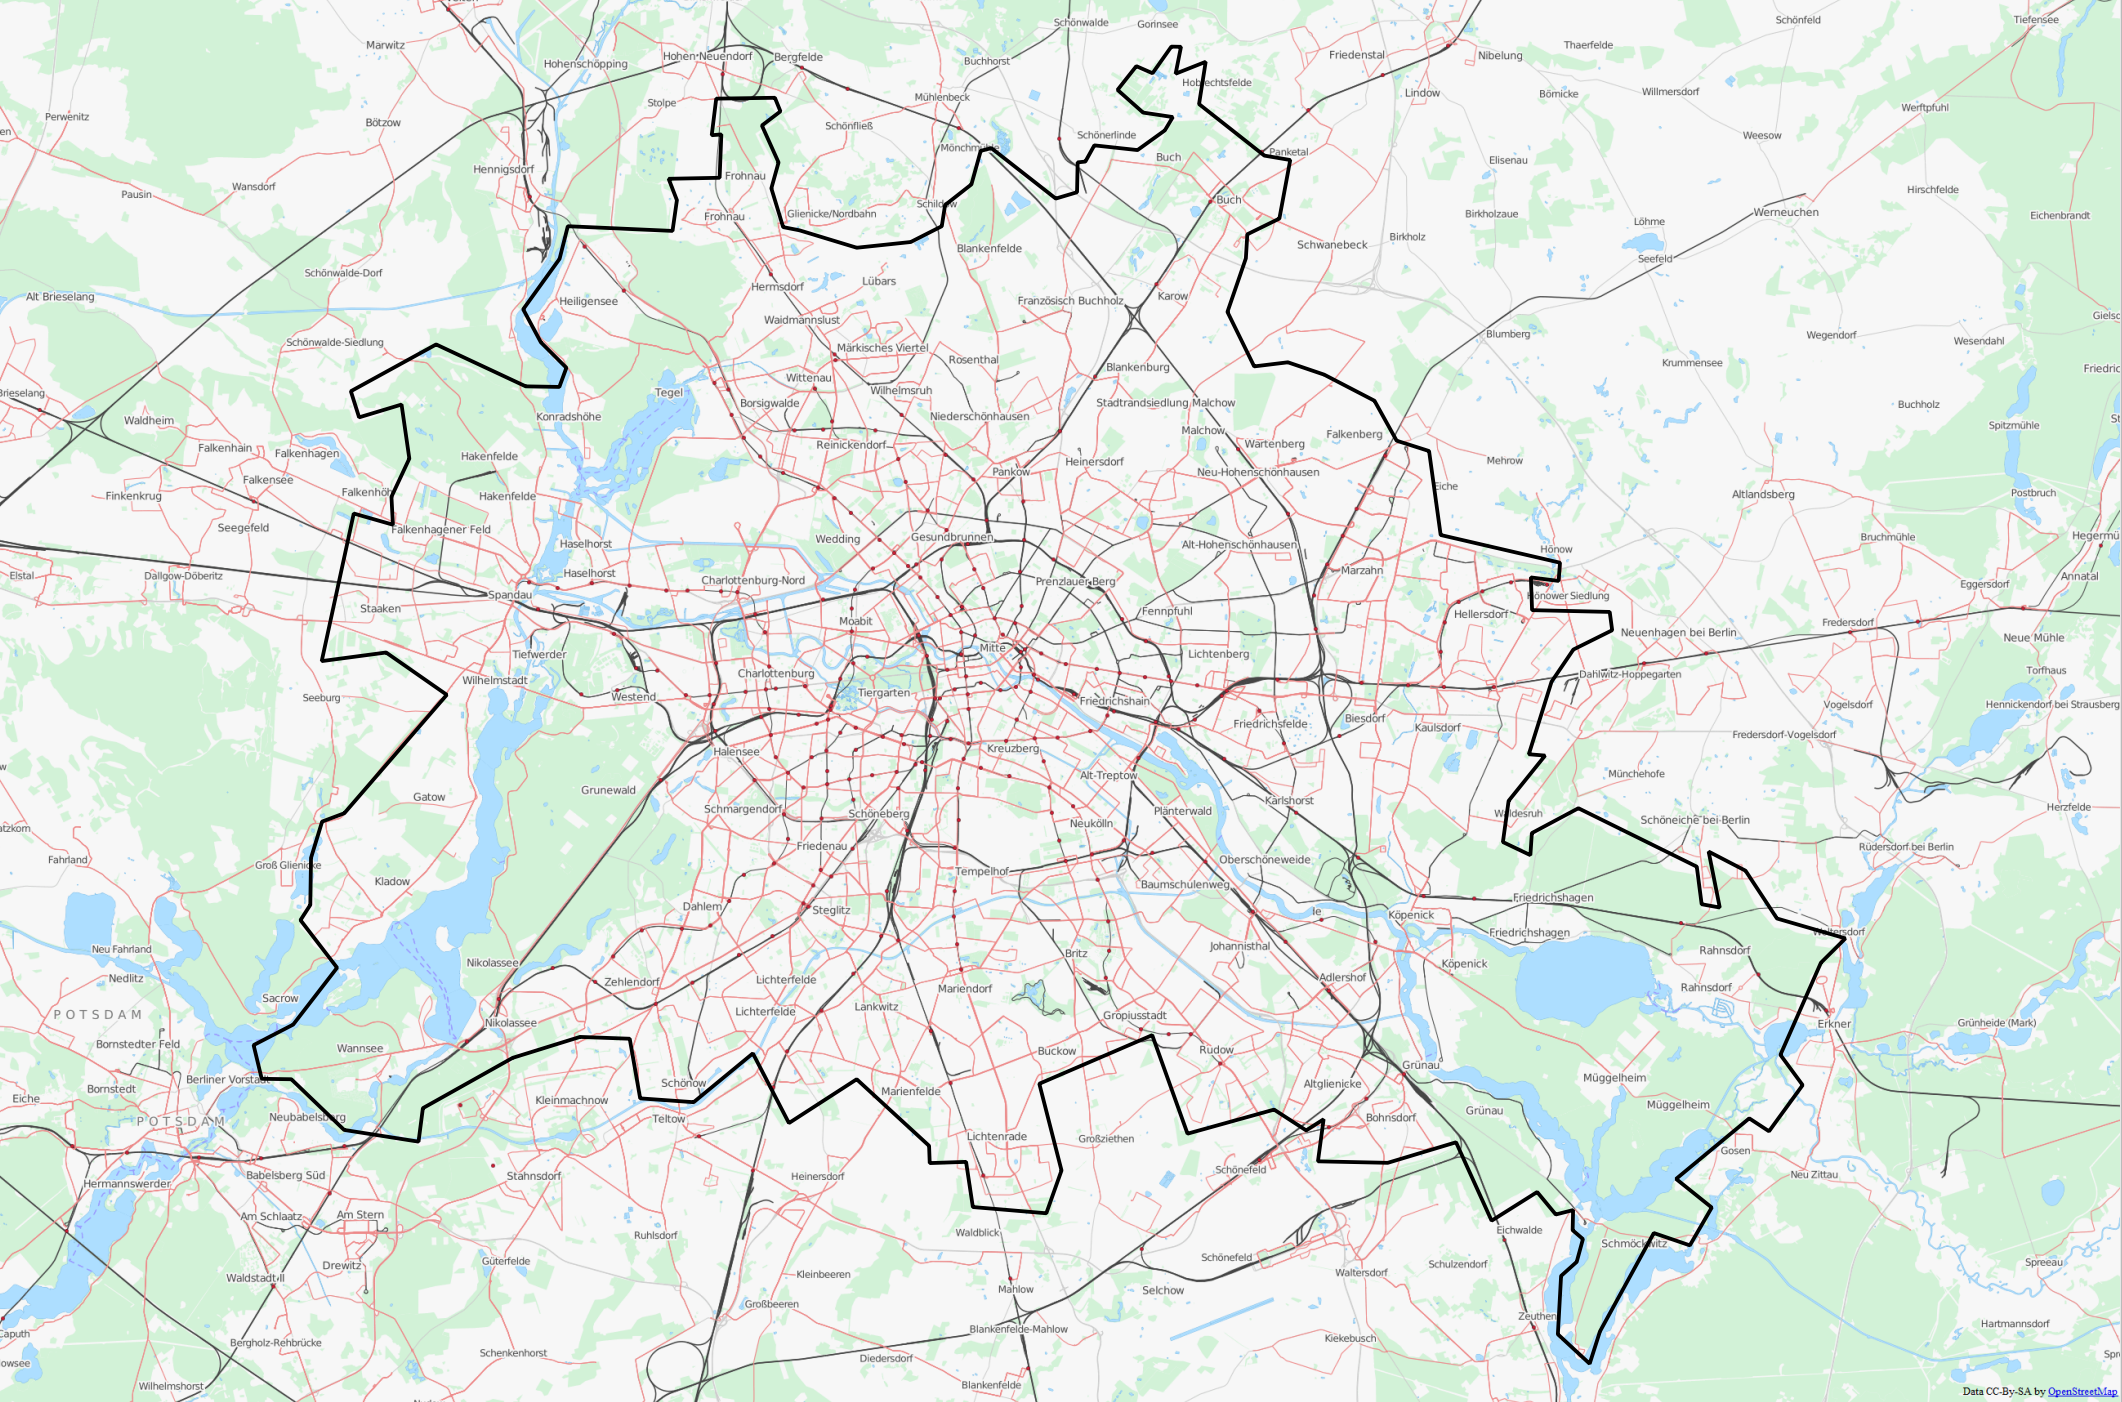
\includegraphics[width=0.99\textwidth, angle=0]{using/figures/berlin_pt}}%
{}
% ------------

% start excerpt from the paper
With the opening of the new international airport of Berlin and Brandenburg BER,
Berlin is expecting some major changes in travel demand. Especially, the
existing airport Tegel, currently exclusively served by buses operated by \gls{bvg},
will cease operations. \gls{bvg} had thus a large interest in a new transport model
for the Berlin area. Due to the big changes, the model should not only deliver
the basis for future planning of the regional transport system, but has to
provide detailed information about passenger flows of different user groups as
well. Such user group specific analyses are considered of high importance for
the \gls{bvg} in order to provide a basis for their future business strategies, which
is why an agent-based model was specifically requested. Two scenarios were
actually asked for, one for the year 2008 (actual state), and one for the year
2015 (prediction). To fulfill the needs mentioned above, the team of 
\citet{PTV2013}, \citet{Senozon2013} and \citet{VSP2013} at Technische Universität Berlin (TU Berlin)
offered a combined model consisting of both a static macroscopic model built with
\gls{visum} as well as an integrated activity-based demand and
dynamic traffic assignment model built with \gls{matsim}. During
the project, attention was given that both models were based on the same data
sources and that both modeling processes interact with each other to allow data
exchange between the two models.
% end excerpt from the paper

In brief, the model contains about 115\,000 links, % 113269
about 15\,000 directed stops, % 14902
6.0~million agents, % 4422012 (sex) 5992771 (/person)
and 539\,public transport lines operated by \gls{bvg} and other companies of the city
of Berlin and the state of Brandenburg. Among others the model features the transport 
modes Besides the transport modes car, For a more in-depth description of the
model, its generation and its calibration, the reader is referred to the work of
\cite{NeumannEtAl2014IatbrPtBerlinBook}. The model has been extensively been used in 
\citet[][Ch 7/8]{Neumann2014PhD} for the development of the minibus module of Section~\ref{sec:paratransit}.

% ################################################################################################################## ok

% ==================================================================================================================
% ##################################################################################################################
\section{Berlin II: CEMDAP-\protect\gls{matsim}-Cadyts Scenario}
\label{sec:berlinII}
\hfill \textbf{Author:} Dominik Ziemke

\editdone{This text has undergone the professional edit. Please no grammatical changes anymore! They are most-probably wrong.}

% ##################################################################################################################
%As explained in section ?????, transport modeling can be considered as the representation of the interaction of transport demand (i.e. people and goods being transported) and transport supply (i.e. transport infrastructure and services) in the transport system. Depending on the application of innovative strategy modules (see section ?????), MATSim accounts for the adaption of transport demand to transport supply \citep{Balmer2007phd}. It is, therefore, crucial to distinguish choice dimensions, which may be adapted during the modeling process (via the application of innovative strategy modules, see section....) and choice dimension whose initial properties are assumed to be correct (e.g. mode shares have to be initially correct in a scenario where the choice of transport modes is not modeled). In the latter case, it is important that respective properties of the transport demand are correct at the start of the simulation (see section Data Requirements - Demand???).
%
To correctly model initial demand properties not included in \gls{matsim} iterations in specific studies (i.e. activity choice), suitable data are needed. Travel diaries containing departure times sequences, mode choice decisions and activity locations are widely used.
%
%A disadvantage of using trip diaries is, however, that all information that is taken from the diaries is by definition not sensitive to policy measures. Also, trip diaries are normally only available for a very small fraction of the population. Another drawback is that, in Germany and the U.S. (and many other parts of the world), the geo-coding of the activity location is considered sensitive information under privacy legislation, and thus increasingly difficult to obtain (cite ZiemkeNagelBhat2015).
However, much of this data source content, particularly location information, is considered sensitive in terms of data privacy legislation and thus increasingly difficult to obtain and process in many areas (e.g.,\,in Germany and the United States) \citep{ZiemkeNagelBhat2015IntegratingCemdapMatsimTransferabilityTRB}.

The \textit{Berlin II scenario} (also referred to as the \emph{CEMDAP-\gls{matsim}-Cadyts scenario} according to applied models in its setup), is the outcome of an alternative approach relying exclusively on freely available and easy-to-obtain input data. Starting points for this scenario are publicly available commuting matrices containing homes and workplaces of workers with social security on the municipality level. Based on this information, it is possible to model morning and evening commuting peaks.

To obtain a full-population demand representation, two further major modeling steps are required. First, in cases like the Berlin case, see below, where commuter matrix spatial resolution is quite coarse, higher resolution \gls{od} information is necessary. Second, a procedure is needed to model secondary activities, i.e.,\,all other activities beyond home and work.

The importance of the first step becomes obvious when looking at the German case; here, the whole city of Berlin, with 3.4\,million inhabitants, is represented by exactly one zone \citep{BA2010Pendlerstatistik}. In the United States, commuting matrices are typically available only on a county-to-county level. Since such location-aggregation-based matrices may become the rule, rather than the exception, in privacy-sensitive societies, a (generalizable) method to attain \gls{od} information at a higher resolution is needed \citep{ZiemkeNagelBhat2015IntegratingCemdapMatsimTransferabilityTRB}. The standard solution would be to estimate an activity location choice model. This, however, is difficult if no trip data to estimate the model is available. \gls{od} matrix estimation studies \citep{ZuylenWillumsenMatrix-from-cnts} suggest that traffic counts may be used to make an initially rough \gls{od} matrix more appropriate for a region. As \gls{matsim} is not based on \gls{od} flows, but on full daily plans, the issue comes down to whether a procedure exists to update these initial full daily plans using traffic counts. In the approach used to create the Berlin II scenario, a procedure proposed by \citet{FloetteroedBierlaireNagel2010Bayesian} and implemented in the software \gls{cadyts}---explained in Chapter~\ref{ch:cadyts})---is applied for this task. Specifically, random draws of possible home and work locations within the home or work municipality given by the commuter matrix are made. Various \gls{matsim} plans, each containing one pair of home and work locations, are created for each agent. Then, the \gls{cadyts} calibration procedure is applied within the iterative \gls{matsim} simulation to select plans and locations more likely to occur with given traffic counts.

As stated above, however, full daily plans (as opposed to mere home-work-home commuting patterns) are needed. Therefore, the second modeling step, the modeling of secondary activities for each individual in the region, needs to be addressed. For the Berlin II scenario, \gls{cemdap} is used to generate initial complete daily plans for each individual. One one hand, however, no \gls{cemdap} parameter set is available for Berlin. On the other hand, and more importantly, one major goal of the study creating the Berlin II scenario was to show its generalizability \citep{ZiemkeNagelBhat2015IntegratingCemdapMatsimTransferabilityTRB}. So, the model parameters of \gls{cemdap} estimated for the Los Angeles region (the estimation context) are retained and then used to generate initial plans for individuals in Berlin (the application context in the current paper), based on Berlin demographic data.

To sum up, home and work municipalities are taken from the commuter matrix. Within these municipalities, a set of (more precisely spatially defined) potential home and work locations are randomly chosen for each agent. Full daily plans incorporating the various potential locations of each agent are generated with \gls{cemdap}, based on a parameter set from another region and local demographic data.

Then, the \gls{cadyts} calibration procedure is used to select those initial full daily plans most consistent with Berlin traffic count data. In other studies, \gls{cadyts} has already been applied to update route choice predictions, both for car \citep{FloetteroedChenEtAl2011BehavioralCalibAndAna} and for public transit \citep{MoyoNagel2013ptNetCalibrationABMTPO}. However, it has not been used to update full daily activity-travel plans, as it was in the procedure that created the Berlin II scenario. 

The Berlin II scenario is an activity-plan-based \gls{matsim} transport model for Berlin based exclusively on freely, or readily, available data. If a commuter matrix, some basic population demographics and traffic counts (or, theoretically, another suitable data source on which to run the calibration procedure) are available for a particular regional context, the approach used to create the Berlin II scenario can be transferred to this context. In fact, the Berlin II scenario itself should be seen as a \emph{transferred model}, because initial plans generated by \gls{cemdap} are based on parameter estimates from another geographic region (the Los Angeles area).

Through a validation based on the Berlin 2008 \gls{srv}, an extensive, regularly-conducted travel survey, the created transport demand representation quality has been successfully tested. So far, the Berlin II scenario exists for a 1\,\% and a 10\,\% population sample of all persons, i.e.,\,including workers without social security, as well as non-working people, aged 18 and above, for the study region. Currently, only motorized traffic is considered. Stability tests, showing that agents' daily plans continue to be chosen when \gls{cadyts} calibration functionality is switched off, have been successfully carried out. This is a clear indication that the scenario is applicable and meaningful for policy studies.

Further improvements, like the addition of public transport and a more realistic representation of the population, are planned. Moreover, similar approaches to integrating activity-travel pattern generators (e.g.,\,the \gls{feathers} model) with \gls{matsim} in transport simulation are planned.

% ##################################################################################################################
%\ah{NOTES: to be removed:
%AN: Szenario entstand aus einer Arbeit zur Nachfragegenerierung. Würde also auch in einen conceptual part passen, anderer Ansatz als die meisten anderen Szenarien ("datensparsam"), Integration von CEMDAP (Modell zur Aktivitätenkettenerzeugung)
%
%Aktivitätenkettenerzeugung: ähnlich zu Tel Aviv Modell
%
%FEATHERS am Beginn -> Vortrag Wiepersdorf
%}

% ################################################################################################################## ok

% ==================================================================================================================
% ==================================================================================================================
\subsection{Switzerland}
\hfill \textbf{Author:} Andreas Horni

The Switzerland scenario was initially created for the project Westumfahrung (Section \ref{sec:wu}). It serves as the base for the very frequently used Z�rich scenario (Section \ref{sec:zhScenario}). 

Two main branches can be distinguished. The first and older one is based on a one to one translation of the Swiss population census \citep[][]{BfS_VZ_2000}, whereas the second one applies approaches from the family of IPF (Iterative Proportional Fitting) reported by \citet[][]{MuellerKAxhausen_TechRep_IVT_2013, Mueller_unpub_LATSIS_2012, Mueller_unpub_ETC_2011, Mueller_unpub_STRC_2011, Mueller_unpub_IATBR_2012}.

% --------
\paragraph{Associated projects:}
Projects based on the Switzerland scenario are \ah{...}.

% --------
\paragraph{Study area:}
The study area covers all of Switzerland. Due to the administrative borders no data for demand and supply are yet available for the adjoining countries, which can lead to boundary effects. This means that studies focusing on the Swiss border area can not be accomplished to date.

% --------
\paragraph{Population and demand generation:}
The population is derived from the Swiss Census of Population 2000 \citep[][]{BfS_VZ_2000}. The complete Swiss population is modeled which results in around 7.5 million persons. 

Home locations are given at hectare level and work locations are known at municipality level from the commuter matrices, a component of the Swiss Census of Population 2000 \citep[][p.35]{BalmerEtAl_ResRep_bdktzrh_2009}. A very good overview in German of the population generation, its initial individual demand and activity locations can be found in \citet{MeisterEtAl_SVT_2009}. Further information is given in \citet[][]{CiariEtAl_STRC_2008, MeisterEtAl_WCTRS_2010, BalmerEtAl_ResRep_bdktzrh_2009, BalmerEtAl_ResRep_datapuls_2010, BalmerEtAl_HEUREKA_2008}.

The travel demand is basically taken from the National Travel Survey for the years 2000 and 2005 \citep[][]{BfS-MZ2005_manual_2006} (Swiss microcensus). This sample however, substantially underestimates freight traffic and ignores cross-border traffic of non-Swiss residents. Freight traffic for whole of Switzerland is to date missing but border-crossing traffic is added as follows. Cross-border traffic is derived from mode-specific hourly origin-destination matrices given by \citet[][]{VrticEtAl_ResRep_UVEK_2007}, which are disaggregated to around 600'000 individual MATSim plans for all of Switzerland, which contain the cross-border traffic that originates \emph{outside} Switzerland. Non-Swiss cross-border traffic starting in Switzerland is supposed to be negligible. 

% --------
\paragraph{Activity locations:}
The activity location data set, comprising more than $10^6$ home, work, education, shopping and leisure locations, is computed from the Swiss Census of Population 2000 and the Federal Enterprise Census 2001 \citep[][]{SwissEnterpriseCensus_manual_2001} providing hectare level information. In MATSim all locations are termed \emph{activity facilities} or in short \emph{facilities}. The generation of facilities is described in \citet[][p.33]{BalmerEtAl_ResRep_bdktzrh_2009}.

% --------
\paragraph{Network:}
For car traffic the MATSim scenario planning networks and navigation networks from Teleatlas \citep[][]{MultiNet_Webpage_2010} and Navteq \citep[][]{Navteq_2011} have been used. The most often used network is the planning network derived from from the Swiss National Transport Model \citep[][]{VrticEtAl_BiegerEtAl_2003}.

Recently, a network for public transport simulation has been added. It is derived from the National Transport Model of the UVEK described by \citet[][]{VrticFroehlich_ResRep_UVEK_2010}. 

% --------
\paragraph{Modes:}
The scenario simulates car and recently also public transport. The schedules for pt are given at the ``regional'' level. Fine-granular schedules are not yet available. The modes walk and bike are ``teleported''. 

% --------
\paragraph{Calibration and validation:}
Calibration is mainly done for modal split and distance distributions. Utility function values are set accordingly.

For validation count data on city level, cantonal level and national level \citep[][]{ASTRA_Webpage_2006} are available from various sources  resulting in 600 links measured for Switzerland. An average working day (Monday to Thursday, excluding public holidays) is used for comparisons in current projects.

\ah{Simulation quality, achieved results}

% ================================================================================================================== \clearpage

% ==================================================================================================================
% ##################################################################################################################
\section{Zürich}
\label{sec:zhscenario}
\hfill \textbf{Author:} Andreas Horni

\editdone{This text has undergone the professional edit. Please no grammatical changes anymore! They are most-probably wrong.}

% ##################################################################################################################
The \gls{matsim} team frequently uses the Zürich scenario, based on the Switzerland scenario described above. The Zürich scenario, however, was more detailed; it was enhanced by data available only for the smaller region; e.g., traffic light data or freight demand data was only included for Zürich city and the canton. It is under continuous development, calibration and validation and has been applied in numerous projects, serving as a real-world research example.   

\citet{HorniEtAl_TechRep_IVT_2011_a} provided a technical overview of the first scenario branch; \citet[][]{BalmerEtAl_ResRep_bdktzrh_2009} described its generation for the "Westumfahrung" project . 

The study area was delineated by a circle, with a 30\,kilometer radius around Bellevue, a central and prominent Zürich location. This delineation led to two versions,  the \emph{Zürich diluted scenario} and the \emph{Zürich cut scenario}. For the first, all agents crossing the study area during the simulated day were considered (Figure~\ref{fig:zurichScenario}), resulting in almost 2\,million agents. For the second, only agents remaining in this area the whole day were modeled. The \emph{Zürich cut scenario} was employed as an experiment in \citet[][]{Hackney_PhDThesis_2009}, but using the \emph{Zürich diluted scenario} for production runs is preferable.

Demand was taken directly from the Swiss model; freight traffic was also added to the Zürich scenario, as follows. Canton Zürich raw freight traffic data was taken from the \gls{kvmzh}, provided by \citet{AMV_Webpage_2011} and documented in \citet[][]{GottardiBuergler_SV_1999}.  Zonal level matrices were disaggregated to single \gls{matsim} plans \citep[][]{ShahM_TechRep_IVT_2010}. Matrices for small delivery and heavy trucks were combined into one activity called \emph{freight}. An additional 180\,000 agents were generated for the Zürich region.

For the diluted Zürich scenario, all Swiss facilities, as described above, were used as activity locations. For the diluted scenario, the networks were not thinned out. For  public transport simulation, network and transport schedules were derived from the \gls{kvmzh}. Walk and bike modes were "teleported". 

Calibration was mainly done for modal split and distance distributions and utility function values set accordingly.

For validation, count data on city level, cantonal level and national level \citep[][]{ASTRA_Webpage_2006} were available from various sources, resulting in 123\,links measured for the Zürich  inner city, delineated by a 12\,kilometer radius around Bellevue. The reduced count analysis radius was applied to reduce boundary effects resulting from demand reduction outside the 30\,kilometer radius study area. An average working day (Monday to Thursday, excluding public holidays) was used for comparison in current scenarios.

Some traffic signal data was available for Zürich city \citep[][]{STAPOZH-DAV_unpub_gtZH_2008}; this was integrated for the Westumfahrung project.
%
\createfigure%
{The diluted Zürich scenario}%
{The diluted Zürich scenario}%
{\label{fig:zurichScenario}}%
{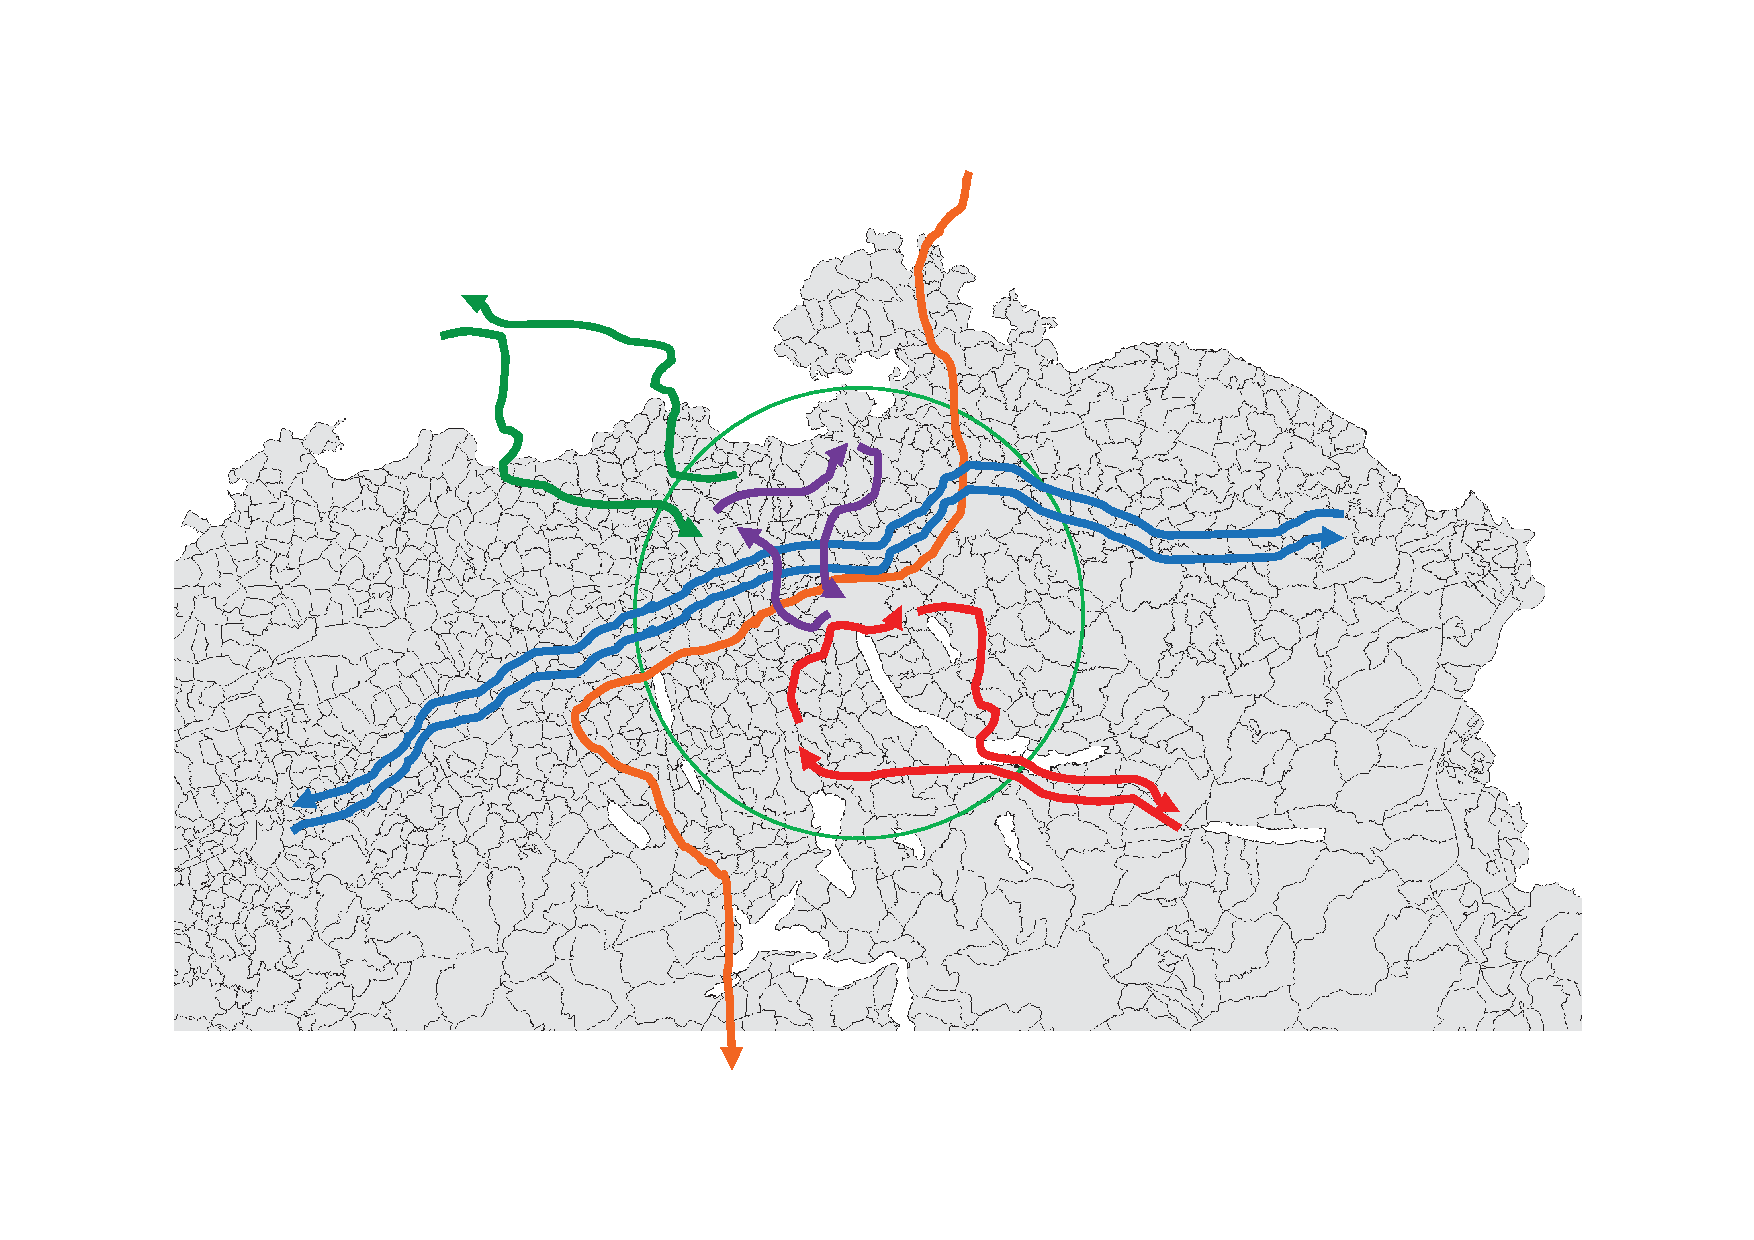
\includegraphics[width=0.99\textwidth, angle=0]{using/figures/zh.pdf}}%
{}

% ##################################################################################################################
 \clearpage

% ==================================================================================================================
% ##################################################################################################################
\section{Singapore}
\label{sec:singapore}
\hfill \textbf{Authors:} Alexander Erath, Artem Chakirov

\editdone{This text has undergone the professional edit. Please no grammatical changes anymore! They are most-probably wrong.}

% ##################################################################################################################
The \gls{matsim} Singapore scenario \citet[][]{ErathEtAl_TechRep_FCL_forth} was implemented and is maintained at the \gls{fcl}, a research program of the \gls{sec} and part of Singapore's National Research Foundation \gls{create}. The scenario covered the whole Singapore area, with a population of approximately 5 million and included traffic  to and from neighboring Malaysia. Singapore provides an excellent study case for an agent- and activity-based modeling approach: a fairly densely populated city, with an extensive public transport infrastructure and advanced transportation and pricing policies. 

% ====================================================================================================
\subsection{Demand}
In the absence of a full-population census for Singapore, a synthetic population was generated based on data from the \gls{hits}~2008 \citep[][]{Choi_JOUR_2010} and population breakdowns of Singapore’s population census~2010. The synthetic population was derived using the fitting and sampling method \citep{MuellerKAxhausen_TRB_2011}, where a reference sample of household and person records was weighted, using an \gls{ipf} technique, until the weighted sample matched marginal census control totals. In our case, the reference sample was from travel survey records; fitting technique was the entropy optimization method proposed by \citet[][]{BarGeraEtAl_TRB_2009} and implemented by Kirill Müller, IVT, \gls{eth} Zürich. Then, the reference sample records were replicated through weighted sampling until the population total was met. 
 
Car ownership was modeled on a household level and driving licenses were assigned to individuals, using discrete choice methods. Given the high car tax in Singapore, the model reflected lower car ownership level than in other developed nations. The model presented in \citet[][]{VanEggermondEtAl_IATBR_2012} included not only socio-economic, but also spatial variables and proved to be essential to the \gls{matsim} Singapore model, leading to accurate mode choice and mode share predictions. 

Activity locations were defined on an individual building level, with  information on building and facility types compiled from various sources:i.e., the land-use master plan \citep[][]{URA_Rep_URA_2008}, government websites and online directories, as well as points of interest information provided by \gls{navteq}. In the absence of a business census, an innovative approach for location identification and corresponding number of work places was developed, drawn from the full smart card data record of public transport journeys and enriched with information on land-use and estimates of building floor space. In a first step, a probabilistic model was applied to a daily public transport journey record to identify types of activities performed between two subsequent public transport trips. Estimated and calibrated using HITS 2008 records, the model combined variables such as time of day, activity duration and land-use around each stop or station to ensure an accurate differentiation between home, work, or other activities. After accounting for mode shares in 53\,different zones, an optimization technique employing accessibility computation was applied to distribute work activities to individual buildings. More details on the newly developed methodology and its practical application were reported in \citet[][]{ChakirovErath_IATBR_2012} and \citet[][]{OrdonezErath_TRR_2013}. 

Assignment of households to buildings was performed using detailed information on residential developments; for public housing, which represented about 80\,\% of Singapore's residential building stock, information on distribution of different dwelling types was employed, while for privately owned condominiums, only information on number of apartments per building was available. Work locations were assigned using a zone-based gravity model using prior estimated number of work activities in each building as additional information for distribution of workplaces within each zone. Activity chains were assigned based on their observed frequency in \gls{hits}, taking into account key socio-demographic parameters like sex, age, occupation and income. Activity chains of type home~--~work~--~home were by far the most frequent, accounting for approximately 50\,\% of the trips.
Freight and cross border traffic, as well as tourist travel demand, were derived based on a set of origin destination matrices provided by the \gls{lta}. These matrices were converted into special daily plans. Information on the temporal distribution of freight trips was derived from loop detector data for freight and temporal attraction profiles of major tourist sites.

% ====================================================================================================
\subsection{Supply}
Using a semi-automatic map-matching algorithm~\ref{sec:networkeditor-singapore}, a high-resolution navigation network provided by \gls{navteq} was map-matched to, and enhanced with, \gls{lta}'s planning network lane and capacity information. Without access to traffic signal cycle time data, traffic lights were not specifically modeled. Extensive attention was paid to public transport modeling; interaction between private and public transport with Singapore’s high density and limited space was very important. Simulating dynamic effects, such as bus bunching, was crucial for obtaining realistic travel times and mode shares. Public transport network and schedule data provided by \gls{lta} included bus and train routes, as well as stop and station location. This information was matched to the road network, using yet another map-matching algorithm presented by \citet[][]{Ordonez_HKSTS_2011, Ordonez_Webpage_2011_4}. Recently, the scenario was updated using public transport schedule data derived from public transport smart card data records \citet[][]{Fourie_TechRep_FCL_2014}. Such schedule information provided actual vehicle dispatch frequencies and headways, which are continuously adjusted and, in some cases, can substantially deviate from published schedules. Additional features of public transport simulation in Singapore’s model included advanced bus dwell time model \citep[][]{SunEtAl_TransResA_2014}, as well as an approximation of the distance-based public transport fare scheme.

Other modes, specifically walking and cycling, were "teleported" with constant travel speeds without any interaction with other users. 

% ====================================================================================================
\subsection{Behavioral parameters}
Behavioral parameters specific to Singapore's context were borrowed from \citet[][]{LTA_unpub_2009} and used with the widely applied Charypar-Nagel function for activity scoring \citet[][]{CharyparNagel2005ga4acts}. Thus, the same parameters were used for all agents, ignoring user preferences heterogeneity and time values in the initial scenario implementation. Furthermore, no additional crowding penalties (impacting travelers' discomfort) were considered at this stage; public transport overcrowding effects were taken into account only with physical vehicle capacity limitations, as well as their implications for dwell time and the bus bunching phenomenon. 

% ====================================================================================================
\subsection{Policy}
The \gls{matsim} model for Singapore also included \gls{erp} scheme, featuring time and vehicle-dependent road pricing. Based on two data sets, with location and time-dependent price levels, prevailing tolls were specified for 73\,network links where toll gantries had been installed, as of February, 2012. To account for the numerous dedicated bus lanes, additional links attributed to exclusive bus use were added to the network. The existing links' capacity was reduced accordingly, even if, in some cases, dedicated exclusive bus lanes by buses existed only during peak hours. Such a simplified setup, insensitive to the time-dynamic operation of dedicated lanes, led to actual road capacity underestimation during periods when bus lanes were also open to other motorized traffic. However, as most links featuring bus lanes consisted of three or more lanes, the effect on modeled traffic conditions during off-peak hours appeared to be low.

% ====================================================================================================
\subsection{Calibration and validation}
Road usage data is available for around 200\, 
%\textbf{EXACT 200?} 
count stations at hourly intervals. Public transport smart card data availability provides an additional validation dimension. For the future,the opening of new \gls{mrt} lines---since setting up the model in 2012---presents a unique opportunity for comparing observed ridership with predicted ridership in the model. However, systematic calibration and detailed validation have not yet been conducted.

% ##################################################################################################################

% ==================================================================================================================
% ##################################################################################################################
\chapter{Munich}
\label{ch:munich}
\hfill \textbf{Author:} Benjamin Kickhöfer

\editdone{This text has undergone the professional edit. Please no grammatical changes anymore! They are most-probably wrong.}

% ##################################################################################################################
The \gls{matsim} scenario for the Munich metropolitan area was set up during 2010.%
%
\footnote{
%
Detailed descriptions of the scenario can be found in \citet{KickhoeferEtAl_VanoutriveVerhetsel_2013} and \citet{Kickhoefer_PhDThesis_2014}.
%
}
%
The main goal was, and is, simulation of local air pollutant and global greenhouse gas emissions and how their levels change with different policy measures---on aggregated and spatially disaggregated levels. Thus the scenario was used for development and testing of the \gls{emt} (see Chapter~\ref{ch:emissions}). For an example illustrating where overall $\mathit{NO_2}$ private car and freight vehicle emissions are produced over one day, see Figure~\ref{fig:munich:no2emissions}.
%
\createfigure%
{$\mathit{NO_2}$ emissions in Munich}%
{$\mathit{NO_2}$ emissions in Munich}%
{\label{fig:munich:no2emissions}}%
{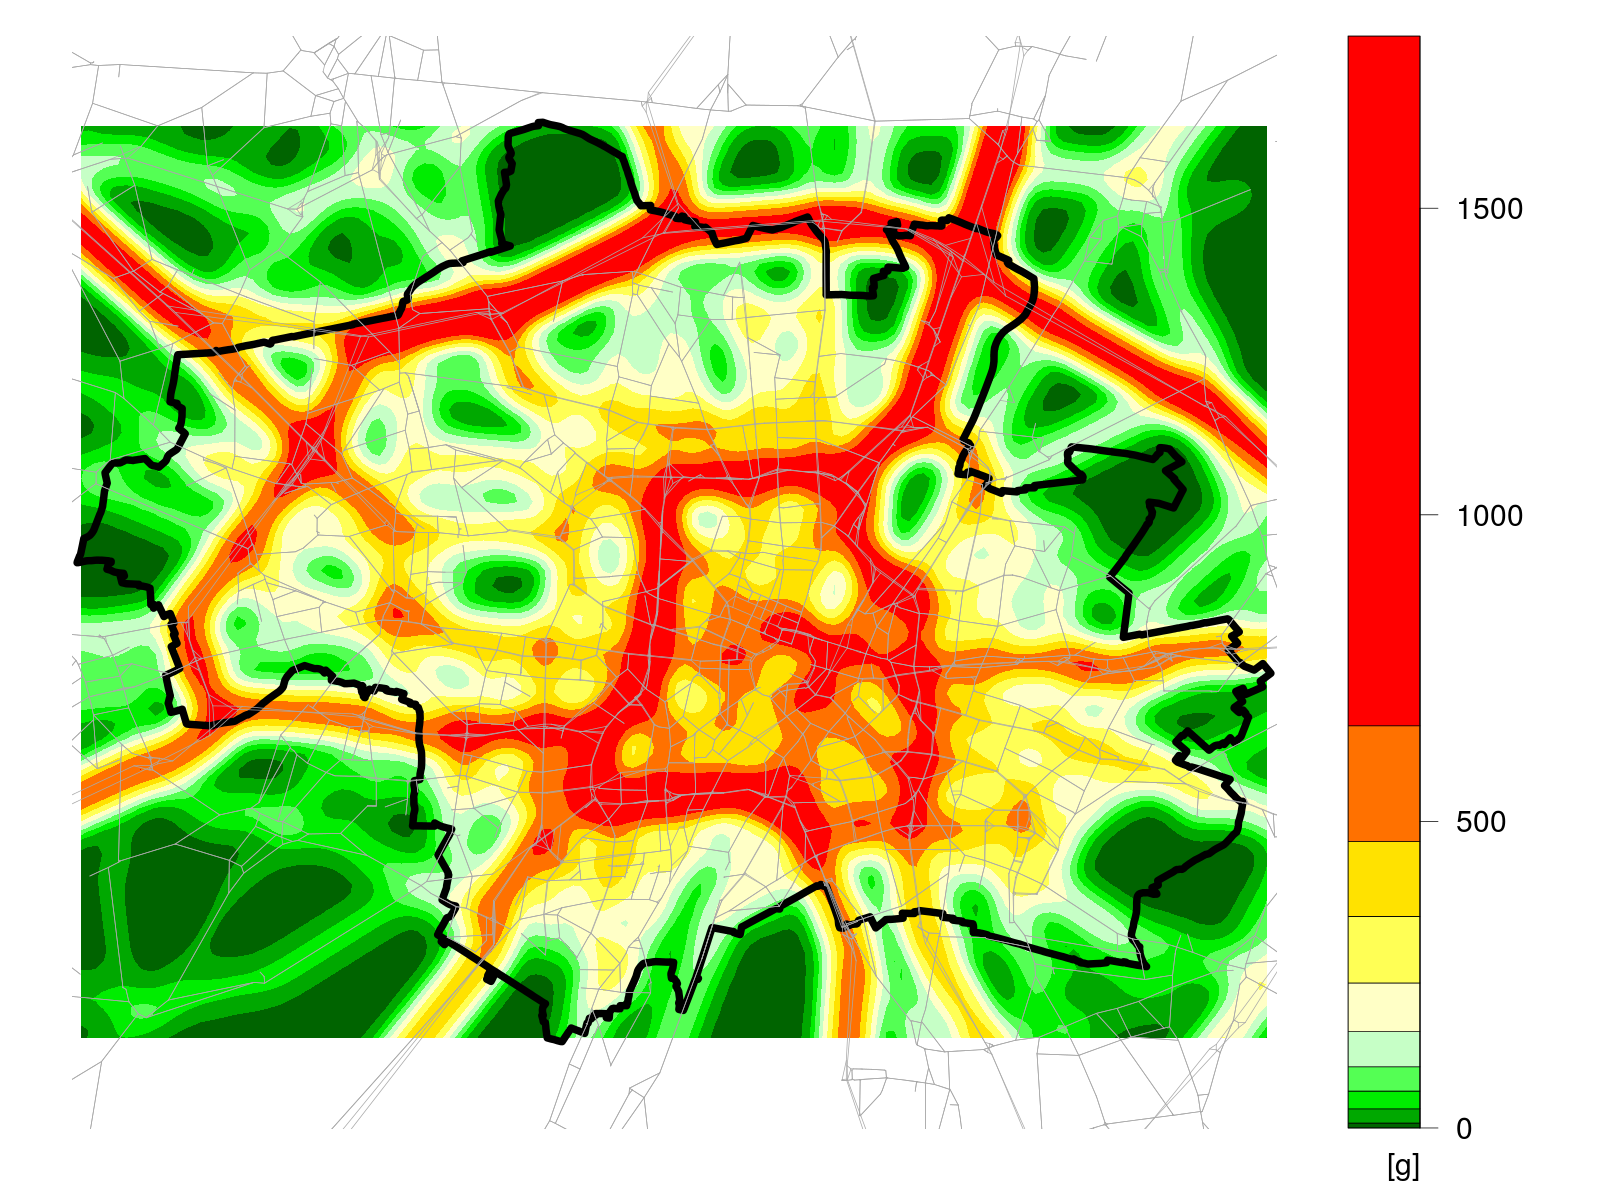
\includegraphics[width=0.85\textwidth, angle=0]{./scenarios/figures/baseCase_1500_NO2_g_108000_0.png}}%
{}

Network information from \acrshort{visum} was converted into \gls{matsim} format, resulting in a network of 17\,888 nodes and 41\,942 links.
%
This transport supply was then linked to travel demand from different sources; an inner-urban traffic activity-based demand from survey data was created, based on \gls{mid} \citep[MiD 2002,][]{FollmerEtAl_TechRep_infasDIW_2004}. This synthetic population segment consisted of roughly 1.4\,million individuals, with detailed vehicle information for every household.
%
Commuters and reverse commuters were modeled with data provided by the German Federal Employment Office \citep{BoehmeEigenhueller_TechRep_IAB_2006}. This part of the population consisted of approximately 0.5\,million individuals, with 0.3\,million commuting to Munich for work. The rest lived in Munich and commuted to their workplace around the city.
%
Freight traffic was also introduced into the model using data from the German Ministry for Transport \citep{ITBBVU_TechRep_2007}. This group consisted of roughly 0.15\,million freight vehicles, performing one commercial trip per day.

The scenario was used for several case studies:
%
\citet{HuelsmannEtAl_LAS_2011} used a single street corridor to validate simulated travel times and emission levels against actual data obtained from a test vehicle.
%
\citet{KickhoeferEtAl_VanoutriveVerhetsel_2013} investigated the relationship between the price elasticities of car travel demand and air pollutant emissions.
%
\citet{HuelsmannEtAl_GerikeEtAl_2013} identified city areas with high air pollution concentration. They defined these areas as ``hotspots'', exceeding the \gls{eu} limits for \gls{no2}. The authors raised toll levels incrementally for vehicles passing these hotspots, until high pollution concentrations disappeared, to estimate true threshold value \gls{eu} avoidance costs.
%
\citet{KickhoeferNagel2012EmissionInternalization} derived time-dependent, vehicle-specific, first-best air pollution tolls to create a benchmark for real-world policy evaluation.
%
\citet{KickhoeferKern_MobilTUM_2014} went one step further and calculated time-dependent, vehicle-specific air pollution exposure tolls to correct toll levels with \citet{KickhoeferNagel2012EmissionInternalization} for a count of individuals affected.



% ################################################################################################################## \clearpage

% ==================================================================================================================
% ##################################################################################################################
\chapter{Sioux Falls}
\label{ch:siouxfalls}
\hfill \textbf{Author:} Artem Chakirov

\editdone{This text has undergone the professional edit. Please no grammatical changes anymore! They are most-probably wrong.}

% ##################################################################################################################
The Sioux Falls scenario provided a convenient test-case, combining fully dynamic demand fitted with realistic socio-economic and demographic attributes with a small-scale road network including an integrated public transportation system. Based on the Sioux Falls road network commonly used for tests and demonstration purposes in transportation literature \citep[][]{BarGera_TNTP_Webpage_2013}, it allowed quick and convenient experiments on new policy or software implementations with \gls{matsim} on a heterogeneous agent population, with a high degree of spatial resolution, but without significant computational requirements. However, it is important to stress that, despite the use of real world data for the generation of the enriched Sioux Falls scenario, it did not aim to replicate the real City of Sioux Falls in South Dakota, US and remains a fictitious test case. Detailed report on scenario generation and its characteristics is provided by \citet[][]{ChakirovFourie_TechRep_FCL_2014} and can also be found at \url{www.matsim.org/scenario/sioux-falls}. 

% ====================================================================================================
\section{Demand}
A realistic, socio-economically and demographically diverse demand population---with  heterogeneous use preferences---was crucial for unlocking the full potential of an agent-based simulation like \gls{matsim}. However, generation of a disaggregated demand description on individual and household levels close to reality was challenging; not only for trip origins and destinations, but also with respect to travel pattern relation and socio-demographic travelers' characteristics.

To address this challenge for the Sioux Falls scenario, and represent the household structure, demographic profile and income distribution as realistically as possible, a synthetic household population, using the \citet[][]{BarGeraEtAl_TRB_2009} entropy optimization technique, was generated. It matched the aggregate distribution of demographic attributes (age, sex and household income) recorded during the 2010 US Census. It contained census tracts inside, and adjoining, the city center of Sioux Falls and was composed of household and person records taken from the (anonymous) 5-year American Community Survey sample (2007-2011), covering 5\,\% of all households.

To keep the scenario accessible, as well as facilitating interpretation and understanding of possible effects on policies studied, only two simple activity chains were initially included: ``home – work – home'' and ``home – other – home''. Activity locations were identified using building stock data set provided by the City of Sioux Falls \gls{gis} division. Each household's home location was assigned randomly to a residential unit within the household's tract. Because no information on the real number and distribution of work places within the relevant area was easily accessible, the static \gls{od} matrix from \citet[][]{LeBlancEtAl_TransRes_1975} was taken as a workplace attraction indicator for each zone. Then, assignment of work places to individual workers, as well as locations of secondary (other) activities, was performed using a parameter-free radiation model presented by \citet[][]{SiminiEtAl_NAT_2012}.

To exploit the full potential of disaggregated demand and add another degree of realism to the scenario, car ownership on the household level was modeled using an ordered probit model, presented by \citet[][]{GiulianoDargay_TransResA_2006} and based on the \gls{npts}~1995. In addition to socio-demographic household characteristics (number of adults, children, pensioners, household income), the model used residential location attributes (population density, public transport access and dwelling type), which better described specific Sioux Falls scenario characteristics, as well as its area-wide bus network. 

% ====================================================================================================
\section{Supply} 
A realistic transportation test network should ensure sufficient complexity of travelers’ choice dimensions while limiting  computational effort. To this end, the Sioux Falls test network was introduced by \citet[][]{MorlokEtAl_ResRep_org-fhwa_1973} and later adapted as a benchmark and test scenario in many publications (see \citet[][]{ChakirovFourie_TechRep_FCL_2014} for overview). The network structure captured the major arterial roads of Sioux Falls, South Dakota, but was never intended to replicate the real city, or all characteristics of its transportation system, such as travel times or modal split. The original network was comprised of 76\,arcs, 24\,nodes and 552\,\gls{od} pairs. For this scenario, road capacities were adjusted according to values provided by the Highway Capacity Manual \citet[][]{HCM_2010} and other related research publications \citep[e.g.,][]{NgCFSmall_Transportation_2012}. The public transportation network added to the scenario included five bus lines, as initially proposed by \citet[][]{AbdulaalLeBlanc_TransScience_1979}, with bus stops placed at regular intervals of 600\,meters. 

Due to the design of \gls{matsim}’s queue simulation, agents were handled only at the beginning and end of each network link and could not enter or leave a link along its length. Therefore, origins and destinations located along very long links led to spatial detail loss, as all origins and destinations along the length of the link were effectively assigned the same coordinates. Consequently, to improve spatial detail level, all links of the Sioux Falls network were evenly split into smaller links, with maximum length of 500\,meters each. Following this operation, number of nodes was increased to 282 and number of links to 334, without changing effective network topology.

In addition to car and bus modes, walking as ``teleported'' mode, with constant travel speeds, and with no interaction with other users, is used as the non-motorized transportation mode. 

% ====================================================================================================
\section{Behavioral Parameters}
Behavioral parameters used in utility functions were based on estimated demand model for Sydney by \citet[][]{TirachiniHensherRose_TransResB_2014}. Before applying parameters in an activity-based context, time-related parameters had to be adjusted to account for utility gained from activity performance. Thus, to provide a value for marginal utility of performing an activity, the travel mode with smallest the disutility was set as a baseline, under the assumption that traveling with this mode was equivalent to idling/doing nothing. Corresponding parameters were split into opportunity costs of time and a mode-specific disutility of traveling, as has in previous \gls{matsim}-related publications as \citet[e.g,][]{KickhoeferEtAl_Transportation_2011}. 

% ====================================================================================================
\section{Results, Drawbacks and Outlook}
Sioux Falls scenario stability and performance was tested using two sets of activity timing constraints, as well as five different random seeds, which all delivered stable and realistic results. \citet[][]{ChakirovFourie_TechRep_FCL_2014} also investigated \gls{mfd} existence and hysteresis characteristics, as discussed in \citet[][]{GeroliminisDaganzo_TRB_2007, GeroliminisDaganzo_TransResB_2008, GeroliminisSun_TransResA_2011}. 

However, recent experience has shown certain coarse network drawbacks; it represented only major arterial roads and neglected minor neighborhood and collector road links. With an elaborate synthetic population and high rush hour demand peaks, the network seemed to be sensitive to network breakdowns under high loading conditions. 

Along with the coarse road network, the coarse public transport network level and the resulting  low level of accessibility (for parts of the population) represented another drawback, particularly relevant to simulation and evaluation of policies sensitive to, or requiring, a certain share of public transport users. 

Replacing the original Sioux Falls network with a finer network obtained from the crowd-sourced \gls{osm} and adding additional public transport lines would address the above-mentioned scenario weakness. However, this introduces a different set of drawbacks and would require further attention. First, the significantly larger number of network links and nodes increases time and resources for routing and dynamic queue simulation and could erase the advantages of a small-scale network. Extended simulation times can be tackled with the new pseudo-simulation methodology, currently developed by \citet[][]{FourieEtAl_TRR_2013}.
Second, total network capacity increase leads to reduction or even disappearance of congestion during peak hours, although including freight and through traffic in the scenario can make it more realistic and address congested conditions during peak-hours. 

% ##################################################################################################################
 ok

% ==================================================================================================================
% ##################################################################################################################
\section{Barcelona}
\label{sec:barcelona}
\hfill \textbf{Author:} Miguel Picornell

% ##################################################################################################################
The Barcelona scenario is one of the three case studies (together with London and Zürich) carried out under the framework of the \gls{eunoia} project. The main goal of the Barcelona case study is to evaluate the impact of different public bike-sharing schemes in the city. The study area covers the metropolitan area of Barcelona, with special focus on the city center, where public bike-sharing stations are located. For this study a novel bike-sharing module was developed by \gls{eth} Zürich.

% ===================================================================================
\subsection{Transport Supply: Network and Public Transport}
The road network has been extracted from the \gls{transcad} model used by the city of Barcelona. Public transport supply has been also considered, comprising: bus, underground, tram, train and bike-sharing. Information about stops and schedules has been obtained from the public information available at the Barcelona Open Data platform as well as from the Barcelona transport authority website. 

% ===================================================================================
\subsection{Transport Demand: Population} 
Agent plans have been defined using anonymised mobile phone registers \glspl{cdr}. From mobile phone data it is possible to identify places where the agents perform activities and their corresponding trips derived from those activities. Activities have been classified as "home", "work" and "other" (including as "other", "leisure", "shopping", etc.). A sample of around 15\,\% of the population has been used in the simulation. Walk, cycling, public transport and car are the modes included in the simulation model.

% ===================================================================================
\subsection{Calibration and Validation}
Different data sources have been used to calibrate and validate the model. First, in order to validate the agent plans obtained from mobile phone data, results were compared to \gls{emef}, leading to conclude that mobile phone data provide similar information than traditional surveys. Additionally, agent’s utility function has been calibrated using the modal split from \gls{emef} and road counts.

% ===================================================================================
\subsection{Results and More Information}
At the time this summary was written, the calibration process ongoing. More detailed information about the scenario and main results can be found at:
\url{www.eunoia-project.eu/publications/} (project deliverables/Report on Case Study 3: Barcelona).

% ##################################################################################################################
 ok

% ==================================================================================================================
% ##################################################################################################################
\chapter{Brussels}
\label{ch:brussels}
\hfill \textbf{Author:} Daniel Röder

\editdone{This text has undergone the professional edit. Please no grammatical changes anymore! They are most-probably wrong.}

% ##################################################################################################################
The \gls{matsim} scenario for Brussels was developed as part of the \gls{sustaincity} project. This project's goal was to couple an urban land use model, in this case \gls{urbansim}, with the \gls{matsim} mobility simulation, to evaluate transport policy impact on urban land use and vice versa. A detailed description of this coupling is given by \citet{Nicolai2013PhD} and others. A detailed description of the scenario development is found in \citet{RoederNagel2013SketchPlanningBrussels}.

The scenario covered the greater Brussels area in Belgium; input data was derived from two main sources. The population was directly generated from the \gls{urbansim} model, covering a total of 860\,214 persons. At home- and at work-locations (per person) were given and converted into a daily home-work-home plan. For computational reasons, a randomly-drawn population sample of one percent was used. \gls{osm} was sourced for the street network generation, which consisted of 10\,861 nodes and 19\,830 links, \ie using mainly the trunk road network.

For the modeling of public transport, two different approaches were tested:  first, the \gls{matsim} default approach for scenarios where no detailed transit schedule is available, based on either: beeline distance and average speed, or network-based freespeed travel times and a designated factor. The second approach was not part of the \gls{matsim} core during the project, but was available as a contribution (\lstinline|matrixBasedPtRouter|). It was based on \gls{od} travel time matrices between transit stops, \ie travel times for all relations were computed in a pre-process. The travel times can based on a real-world-schedule or certain assumptions which can take spatial coverage into account. Advantages of this model are obvious; on one hand, it may depict spatial coverage with public transport supply---here, distance to the next transit stop influences travel time. On the other hand, it may depict the real network, \ie routes and lines and possible waiting times for switching. Both approaches were compared against travel times and mode share measures from a \gls{saturn} model. Since the matrix-based approach came closer to this model, further investigations were based on that.

To evaluate the model's sensitivity to certain policies, a cordon toll scenario was set up, where a toll is charged between 6 and 10\,am every time a car passed a cordon border. \ie every time a car entered a link crossing a cordon border defined by the Brussels freeway ring. Accessibility was calculated and compared for both scenarios.  \citet{RoederNagel2013SketchPlanningBrussels} provides a detailed analysis.

% ##################################################################################################################
 ok

% ==================================================================================================================
% ##################################################################################################################
\section{Cape Town}
\label{sec:capetown}
\hfill \textbf{Author:} Johan Joubert

% ##################################################################################################################
https://matsim.atlassian.net/wiki/display/MATPUB/South+Africa

% ##################################################################################################################

% ==================================================================================================================
% ##################################################################################################################
\chapter{Cottbus: Traffic Light Simulation}
\label{ch:cottbus} \hfill \textbf{Authors:} Joschka Bischoff, Dominik Grether \editdone{This text has undergone the professional edit. Please no grammatical changes anymore! They are most-probably wrong.}

% ##################################################################################################################
The Cottbus (Germany) scenario (Figure~\ref{fig:scenarios:cottbus_location}) is used for traffic light simulation (see Chapter~\ref{ch:signalslanes}). 
It is explained well in \citet[][pp.~87]{Grether_PhDThesis_2014}; this chapter briefly reviews the main points. 
The scenario data is generally available to the public.

The network is derived from \gls{osm} data in summer, 2010 \citep{Bischoff2010BaSylvia} and 
covers all streets within the city boundaries, as well as main roads in the surrounding Spree-Neiße administrative district . 
It is designed as a 100\,\% sample. 
The population is based on the German federal employment agency commuter statistics for both Cottbus and Spree-Neiße \citep{WiethoelterBogaiCarstensen2010IABPendlerberichtBB}. 
As such, the population has only home-work-home plans spread over the usual commuting times, resulting in two peaks, including 
33\,479 agents traveling exclusively by car. 
The scenario is generally not very busy; the area does not usually have major congestion issues.

Figure~\ref{fig:network_municipalities_cottbus_landuse} shows the network over the 
``Corine Land Cover'' landuse \citep{CorineLandCover2006Data}, provided by European Environmental Agency. 
Woods and agricultural areas are depicted; most of the region is agricultural use area.  
Virtual persons in \gls{matsim} need a geographic coordinate for their activities. 
If this coordinate is drawn randomly (solely based on municipality borders), home and work activity locations are uniformly distributed over  the area, \ie most of them in woods and fields. 
Thus, activity locations are drawn randomly in combination with land use data. 
The coordinate must be in the municipality area and for home activity, it must be located in urban fabric areas; for work locations, industrial or commercial areas are also allowed. 
The resulting home activity locations are shown in Figure~\ref{fig:cottbus_population_home}. 

The scenario contains data for 22\,traffic signals within the city center, based on the city's 2009~signal plans; junction layout is also modeled in detail. Fixed-time control data is taken from \citet{KoehlerStrehler2010SignalDemandOptimization}.  
Due to higher transport network resolution, several originally recorded fixed-time control schedules are invalid and were removed; data for 22\,junctions is available. 
Figure~\ref{fig:cottbus_network_signal_locations} shows their transport network location.  

Public transit, not part of the original scenario, is available based on 2011~schedules, although it is not currently used. 
%\createfigure%
%{Cottbus scenario: Geospatial location within Germany, Europe}%
%{Cottbus scenario: Geospatial location within Germany, Europe}%
%{\label{fig:scenarios:cottbus_location}}%
%{%
%  \createsubfigure%
%	{Geospatial area of Brandenburg within Germany, Europe (Red); City of Berlin (Yellow)}
%	{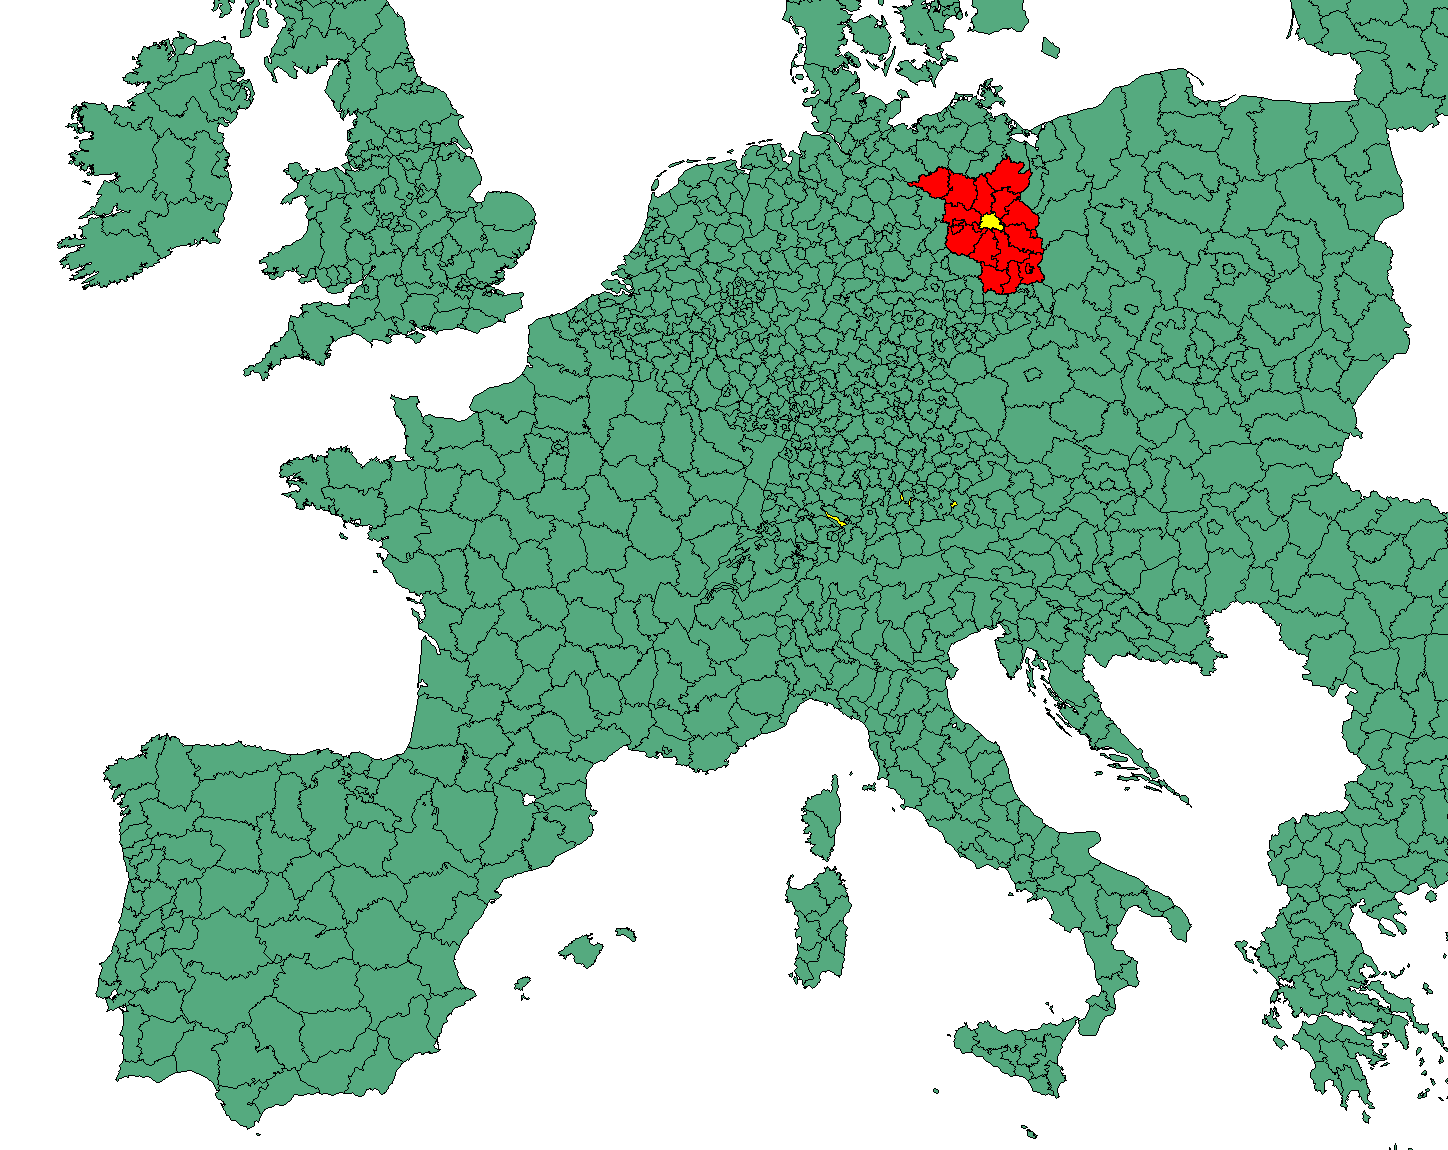
\includegraphics[width=0.49\textwidth]{./scenarios/figures/brandenburg_europe.png}}
%	{\label{fig:scenarios:cottbus_brandenburg_europe}}
%  \createsubfigure%
%	{Geospatial area of Cottbus (Dark Red), within administrative district Spree-Neiße, Brandenburg (Light Red)}
%	{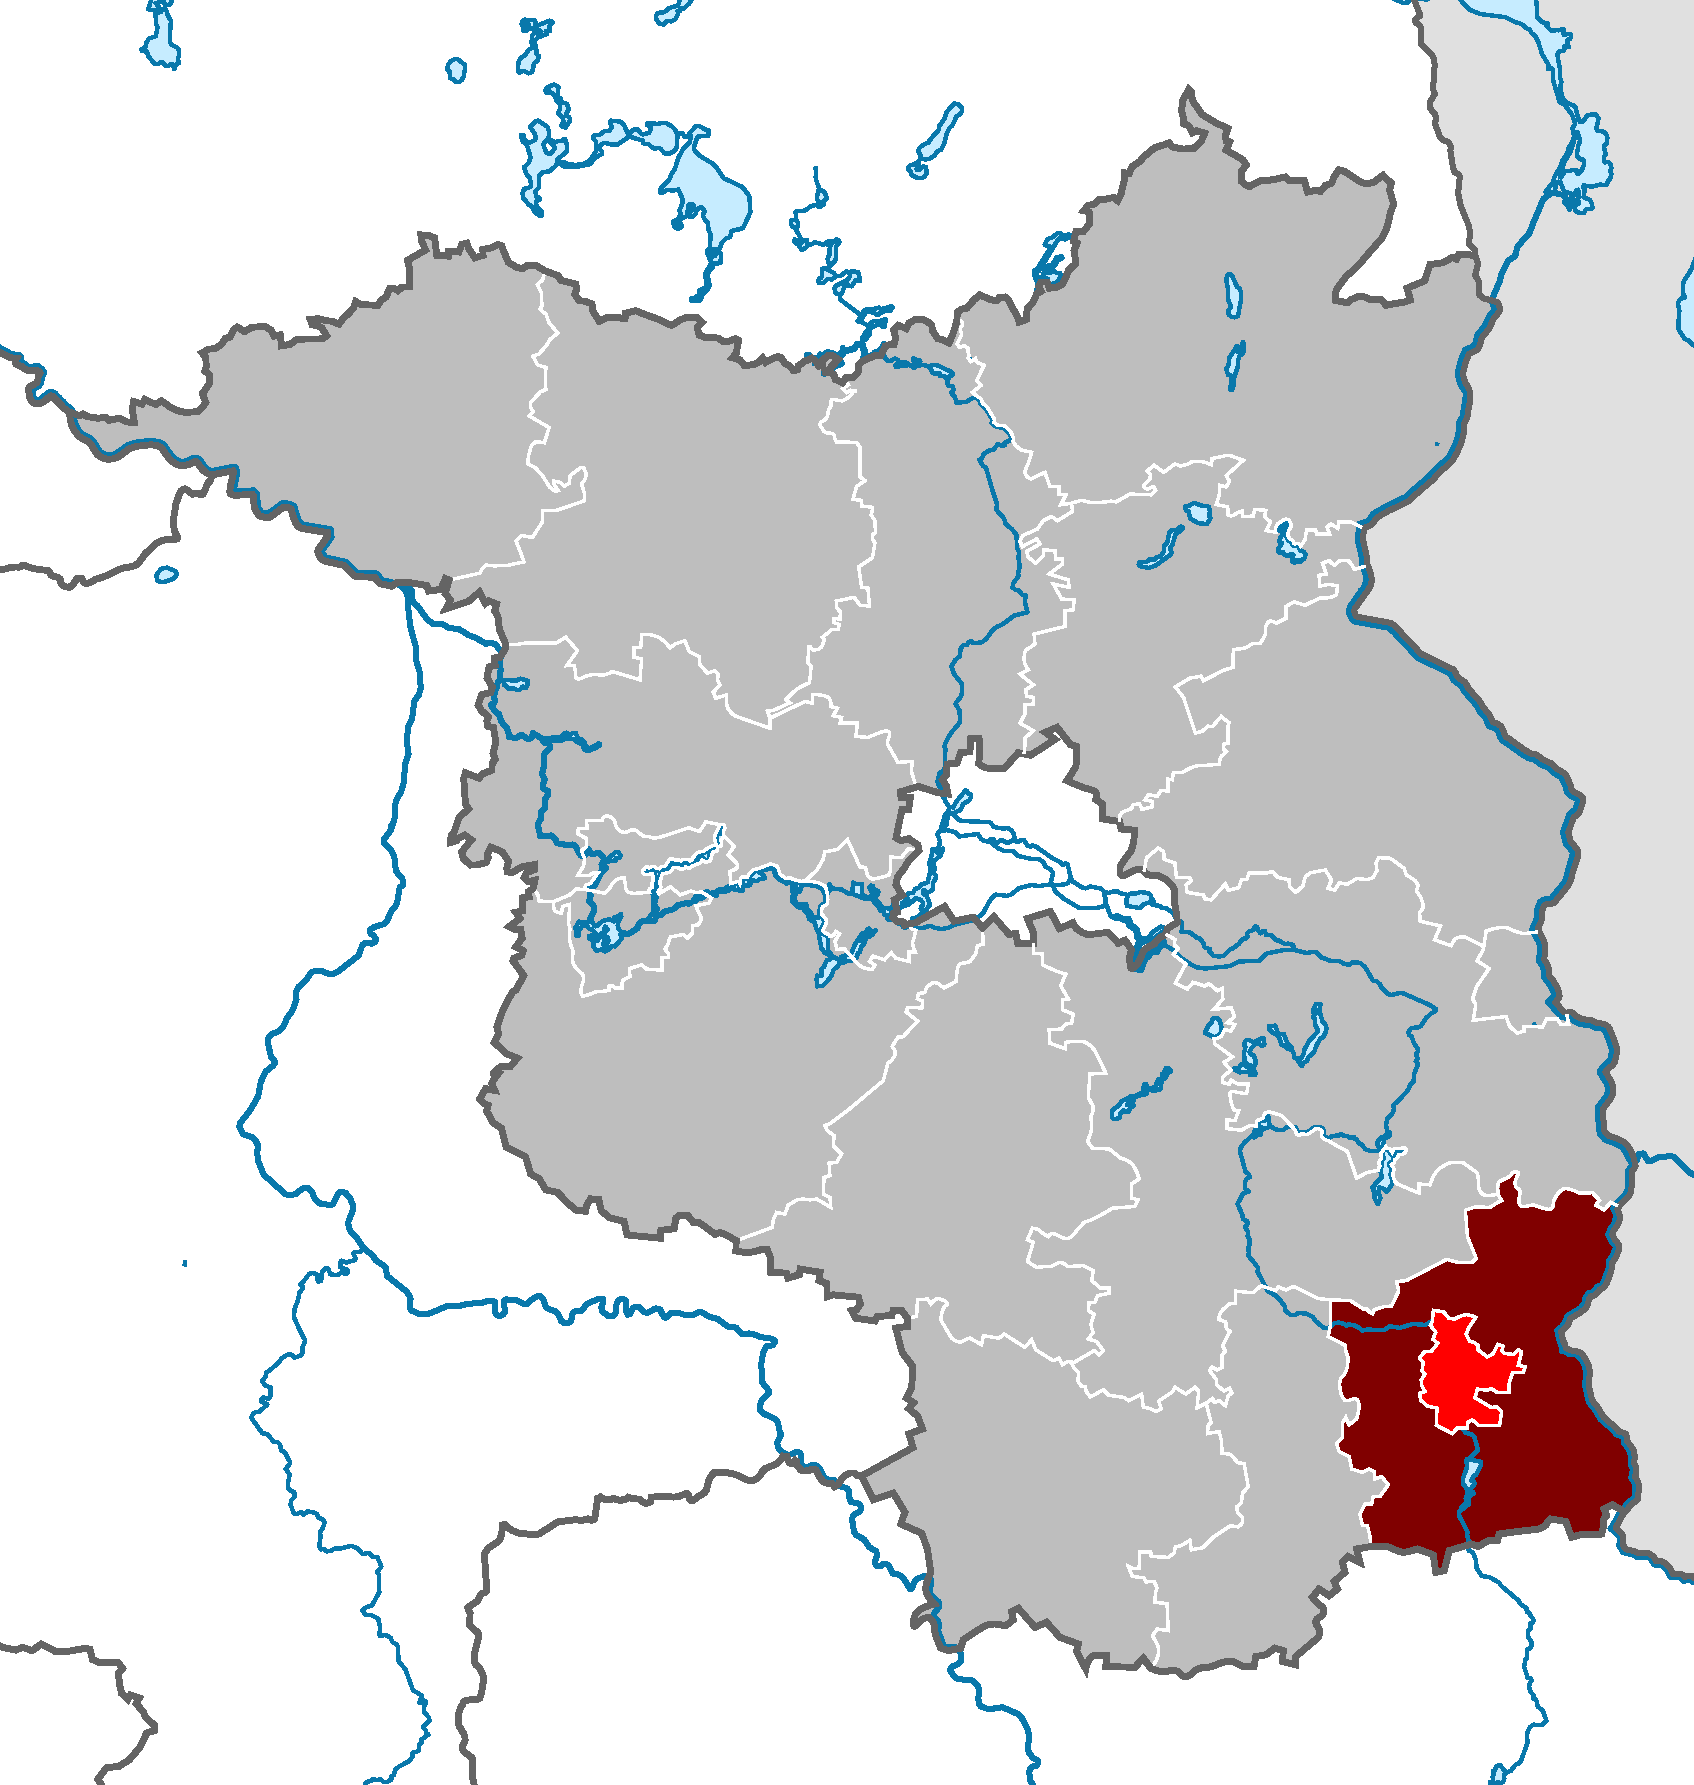
\includegraphics[width=0.49\textwidth]{./scenarios/figures/brandenburg_spree_neise_cottbus.pdf}}
%	{\label{fig:scenarios:cottbus_bb}}
%}%
%{\citet{Grether2014PhD}}

\createfigure%
{Cottbus scenario: Network and population}%
{Cottbus scenario: Network and population}%
{\label{fig:cottbus_network_population}}%
{%
  \createsubfigure%
	{Cottbus network and municipality borders}
	{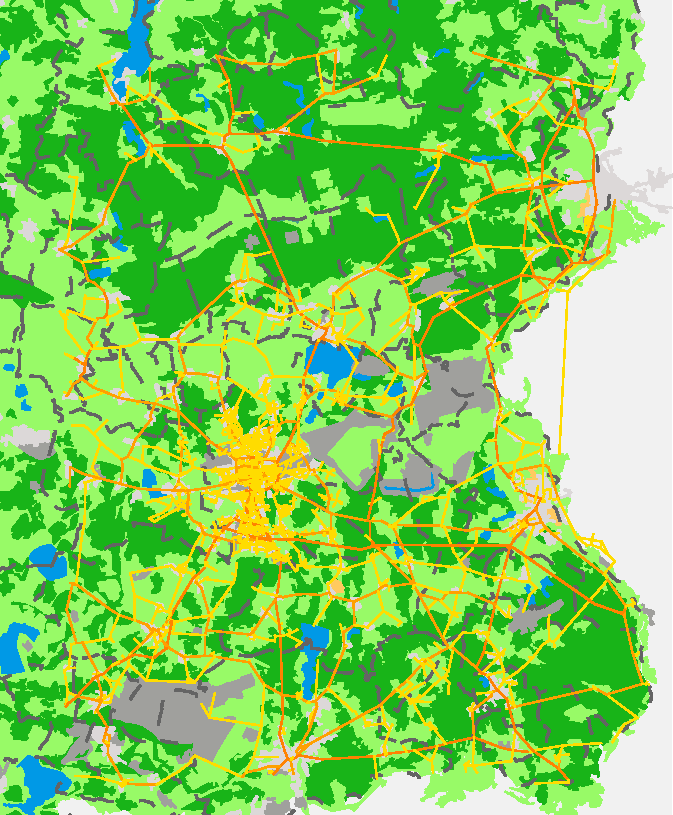
\includegraphics[width=0.49\linewidth]{./scenarios/figures/2013_network_gemeinden_landuse_edit.pdf}}
	{\label{fig:network_municipalities_cottbus_landuse}}
  \createsubfigure%
	{Synthetic population for the Cottbus scenario, geospatial location of home activities}
	{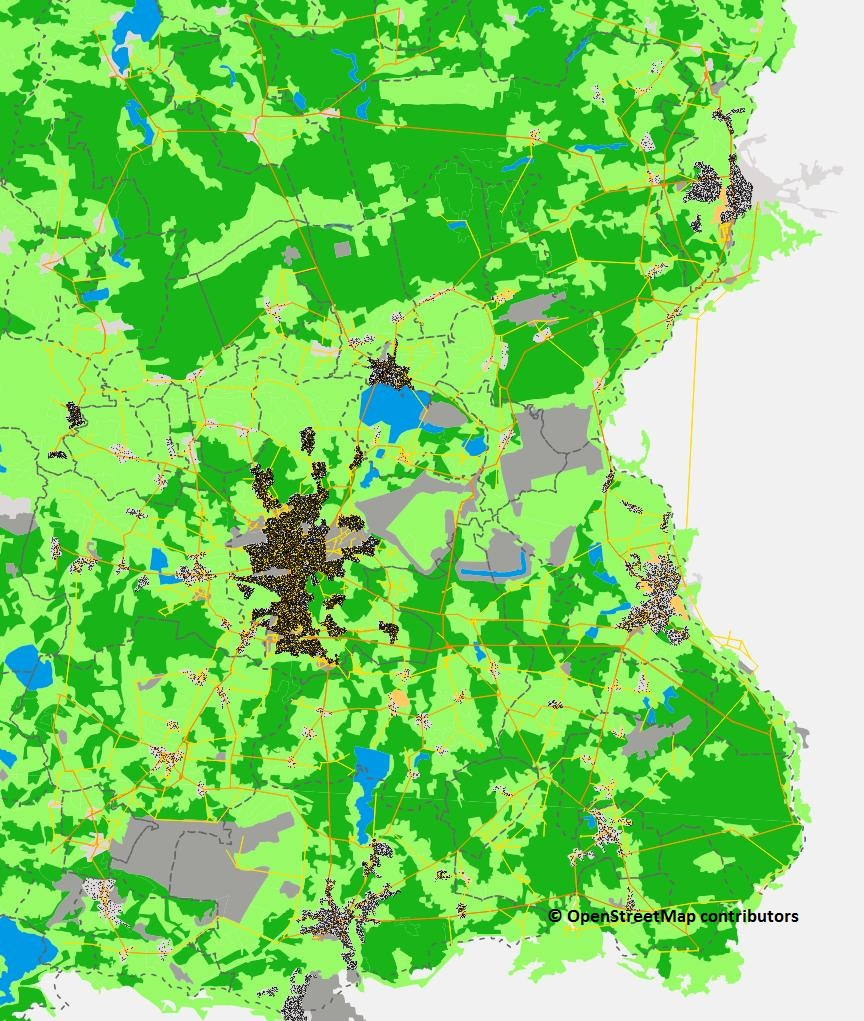
\includegraphics[width=0.49\linewidth]{./scenarios/figures/2013_network_gemeinden_landuse_population_home.jpg}}
	{\label{fig:cottbus_population_home}}
}%
{Source:~\citet{Grether2014PhD}} 

\createfigure%
{Cottbus scenario: Network, area with traffic signals within the city of Cottbus}
{Cottbus scenario: Network, area with traffic signals within the city of Cottbus}
{\label{fig:cottbus_network_signal_locations}}
{%
  \createsubfigure%
	{Location within city of Cottbus}
	{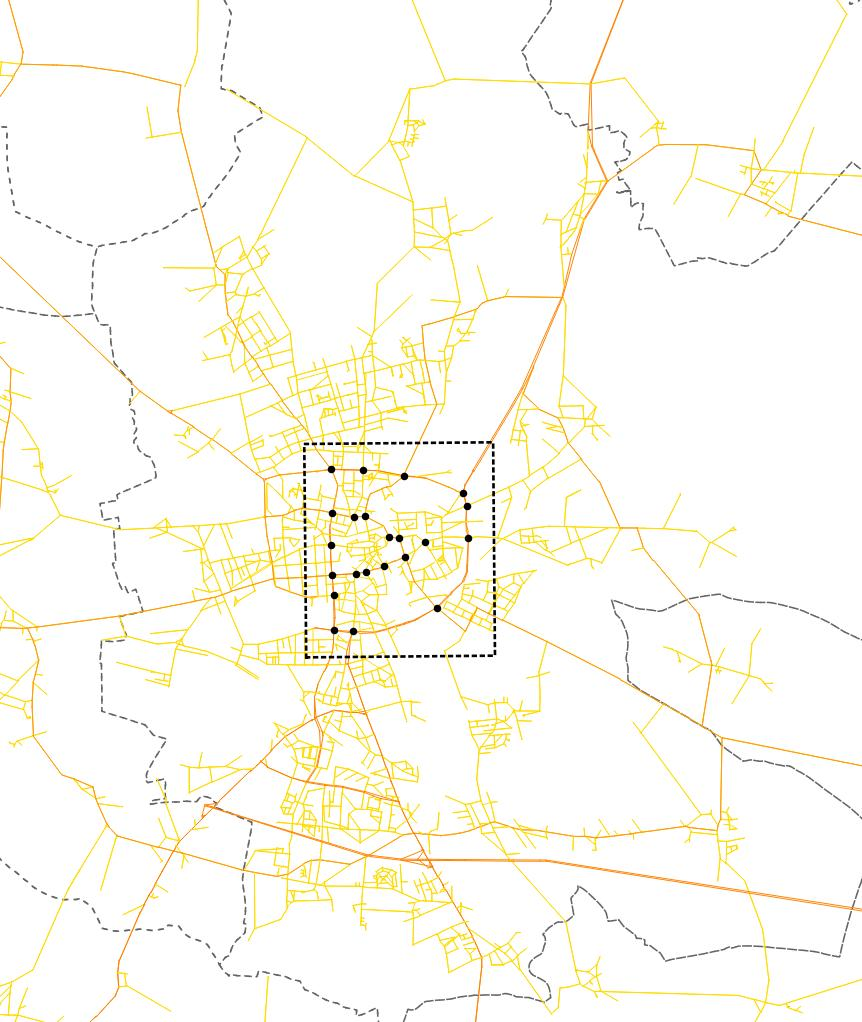
\includegraphics[width=0.49\linewidth]{./scenarios/figures/2013_cottbus_network_signals.jpg}}
	{\label{fig:cottbus_network_signals}}
  \createsubfigure%
	{Signalized area in detail}
	{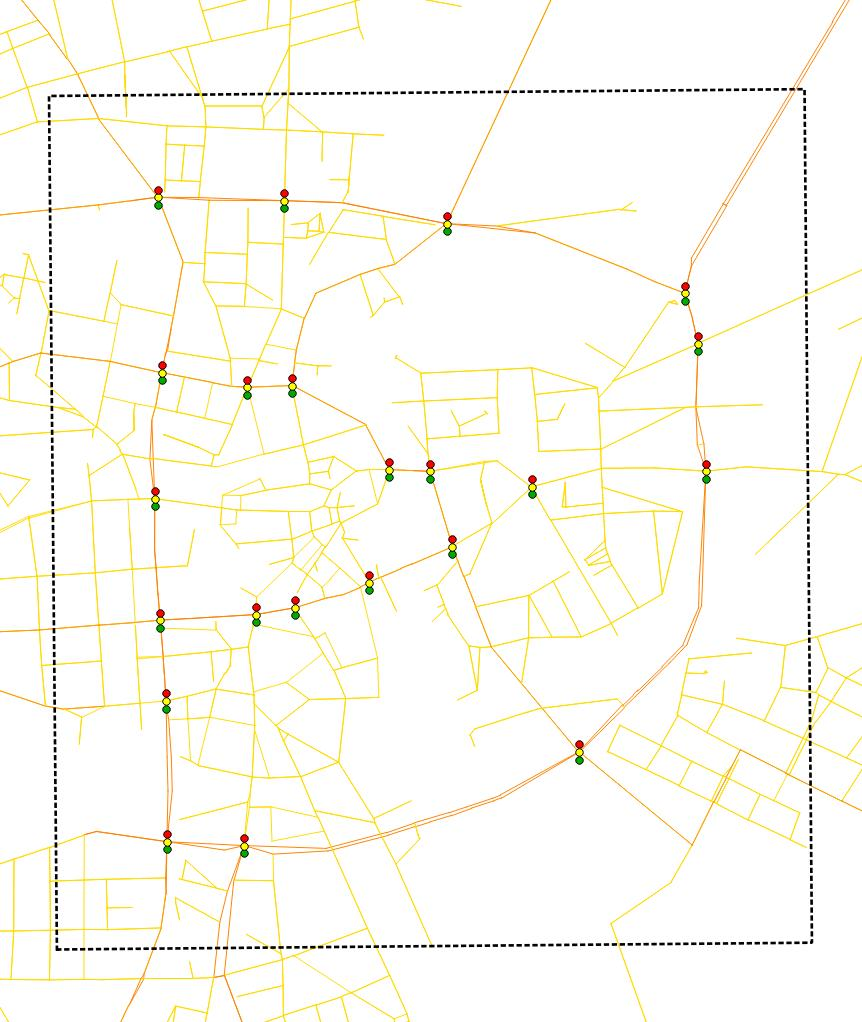
\includegraphics[width=0.49\linewidth]{./scenarios/figures/2013_cottbus_network_signals_zoom.jpg}}
	{\label{fig:cottbus_network_signals_zoom}}
}%
{\citet{Grether2014PhD}}

% ##################################################################################################################

% Andreas Neumann-Mail: frei verfügbar. ÖV vorhanden, 100\% Szenario, das sich mit einigermassen geringem Aufwand rechnen lässt. Grundlage für Dominik G.s Ampelpart
 

% ==================================================================================================================
% ##################################################################################################################
\section{Dublin}
\label{sec:dublin}
\hfill \textbf{Authors:} Gavin McArdle, Eoghan Furey, Aonghus Lawlor, Alexei Pozdnoukhov

\editdone{This text has undergone the professional edit. Please no grammatical changes anymore! They are most-probably wrong.}

% ##################################################################################################################
\subsection{Introduction}
To demonstrate a new spatial choice model, a micro-simulation of urban traffic flows for the greater Dublin region was implemented using \gls{matsim}. The scenario simulated leisure activities and commuting trips completed by individuals using private cars over a twenty-four hour period. For commuting trips, detailed information from the Irish Census was used; a new spatial choice model, inspired by the radiation model, was developed for leisure trips. The effectiveness of the approach was validated using hourly data from count stations on the main motorways around Dublin City. The results show that the micro-simulation accurately reproduced traffic volumes.

% =======================================================================================
\subsection{Study Area}
County Dublin, in Ireland, covers an area of approximately 115\,square kilometers and encompasses several administrative areas. Dublin is a coastal county with the Irish Sea lying to the east. To capture both intra-city and inter-city flows, the scenario considered individuals who live or work in Dublin, capturing those who commute to or out of Dublin, as well as those who live and work there.

% =======================================================================================
\subsection{Network}
To capture the desired study area for the scenario, the network consisted of all roads in the greater Dublin region and major roads for the remainder of the county. The road network was a mix of motorway, national routes and local roads and was extracted from \gls{osm}, along with other information such as speed limits and number of traffic lanes. This \gls{osm} network was prepared for use in \gls{matsim}.  This study focused on private vehicles; the public transport network was not considered, but can be incorporated into the micro-simulation in future studies.

% =======================================================================================
\subsection{Population Generation}
The population for this scenario consisted of all car drivers who live or work in the greater Dublin region and was prepared from a variety of data sets. To obtain home and work locations, the 2011 Irish census was used, particularly census subset \gls{powscar}. This provided home and work locations, mode of commuting transport used, time of departure for work or school and a variety of socio-economic data at an individual level. The individuals relevant to this scenario (drivers who live or work in Dublin) were extracted from the data set. In \gls{powscar}, home locations were anonymized by aggregating them into a statistical unit called the small area, consisting of 80 to 100\,households.  In the greater Dublin region, this represented a street or an apartment complex. We translated this to an individual address point by selecting a random address point within the small area. For this process, we used a commercial database of addresses and their coordinates in Ireland called Geodirectory. To account for non-workers, we used census statistics on spatial distribution of the number of sick, unemployed, retired persons and car ownership to produce the non-working population for the greater Dublin region. These were also assigned to individual address points, providing us with a population of 600\,000 agents for the scenario (see Figure~\ref{fig:dublin0}).

% ======================================================================================= 
\subsection{Demand Generation}
Individuals from the population were assigned work and school locations according to \gls{powscar} (Figure~\ref{fig:dublin0}). In \gls{powscar}, work and school locations were given at a 250\,meters grid level and then translated into an individual address point using Geodirectory. For school and collage locations, the address point was checked using \gls{nace} Codes, to confirm its status as an educational institute. Departure times for work  and school were assigned using a Gaussian curve centered at the declared 30\,minute departure time from \gls{powscar}.  \gls{ints} was used to create non-commuter demand for the road network. Through a survey, the \gls{ints} collected a 24\,hour travel diary for an Irish population sample recording journey origin, destination, departure time and mode. We extracted the private car mode and combined the data with the commuter data to create a 24\,hour activity chain for each individual in the population.

% ======================================================================================= 
\subsection{Activity Locations}
A set of activity locations were obtained from an in-car navigation system’s \glspl{poi} database and augmented with additional \glspl{poi} from \gls{osm}. While work locations were assigned from demand generation, locations for secondary activities, such as shopping and leisure, were not specified in the \gls{ints} and so had to be modeled to create spatial and temporal activity chains for the population. We developed a radiation model variant that applied emission-absorption ideas to compute interaction probabilities for a set of origins and destinations. The radiation model was parameter-free and distance decay was replaced by a ranked-based decay \citep[][]{SiminiEtAl_NAT_2012}. While generally used for modeling movement between regions or cities, we used this approach to produce probabilities of selecting different locations capable of fulfilling a given activity. Where the radiation model uses known populations of locations to produce region ranking, we used attractiveness scores for areas and facilities that could fulfill an activity. A facility, venue or area's attractiveness was derived from venue size, which was calculated using domain knowledge and the model was calibrated with trip distribution patterns from social media check-in statistics. This radiation model variant was used to assign locations to secondary activities in the agents’ day chains for the Dublin scenario demand.

% ======================================================================================= 
\subsection{Validation and Results}
Network, population and demand data were prepared for use with \gls{matsim}. For efficiency reasons, a 25\,\% sample of the population was used for the simulation. The location choice model described above was used to generate the initial demand. On each interaction of the simulation, agents could be rerouted or rescheduled according to the \gls{matsim} default settings, but the locations defined in activity chains remained constant. The simulation reached a stable state after 350\,iterations. The road volume data output was scaled according to the sample used, aggregated to an hourly count and compared to the observed count data from 6\,count stations on motorways around Dublin. In order to compare the effect of the new location choice model, the simulation was re-run using the \gls{matsim} nearest neighbor algorithm for selecting secondary activities' locations.

% =======================================================================================
\subsection{Achieved Results}
Aggregated hourly counts were compared with those observed at the 6\,count stations which determine vehicles traveling in two directions. A typical hourly distribution was obtained by averaging mid-week traffic volumes for a 3\,month period. The results produced by the radiation model showed a stronger correlation between simulated and observed counts than those from the nearest neighbor approach. Figure~\ref{fig:dublin1} showed hourly observed and simulated count data for two count stations; the inset showed relative percentage error for the two approaches being tested. The results indicated that both techniques were effective for estimating commuter traffic during morning and evening peaks. This was to be expected as the location of school and work activities were provided from real world data, but it did confirm the \gls{matsim} routing algorithm effectiveness For daytime traffic, which consisted mostly of secondary activities, our variant of the radiation model outperformed the nearest neighbor approach; it included individuals who were willing to travel further for better opportunities, producing more accurate results.

% =======================================================================================
\subsection{Associated Projects and Where to Find More}
The Dublin scenario validation results demonstrated the effectiveness of \gls{matsim} as a traffic simulation tool and also showed the power of our spatial choice model which adapted the radiation model to predict individual movement at a small spatial scale. In the future, the research will be expanded by considering a \gls{multimodal} transport network and scaling the scenario from an urban simulation to a national one. Full details of the Dublin scenario can be found in \citet[][]{McArdleEtAl_IWUC_2012} and \citet[][]{McArdleEtAl_ACMTIS_2014}.

% =======================================================================================
% ------------
\createfigure%
{The distribution of work and home locations for part of the Dublin scenario}%
{The distribution of work (upper image) and home (lower image) locations for part of the Dublin scenario}%
{\label{fig:dublin0}}%
{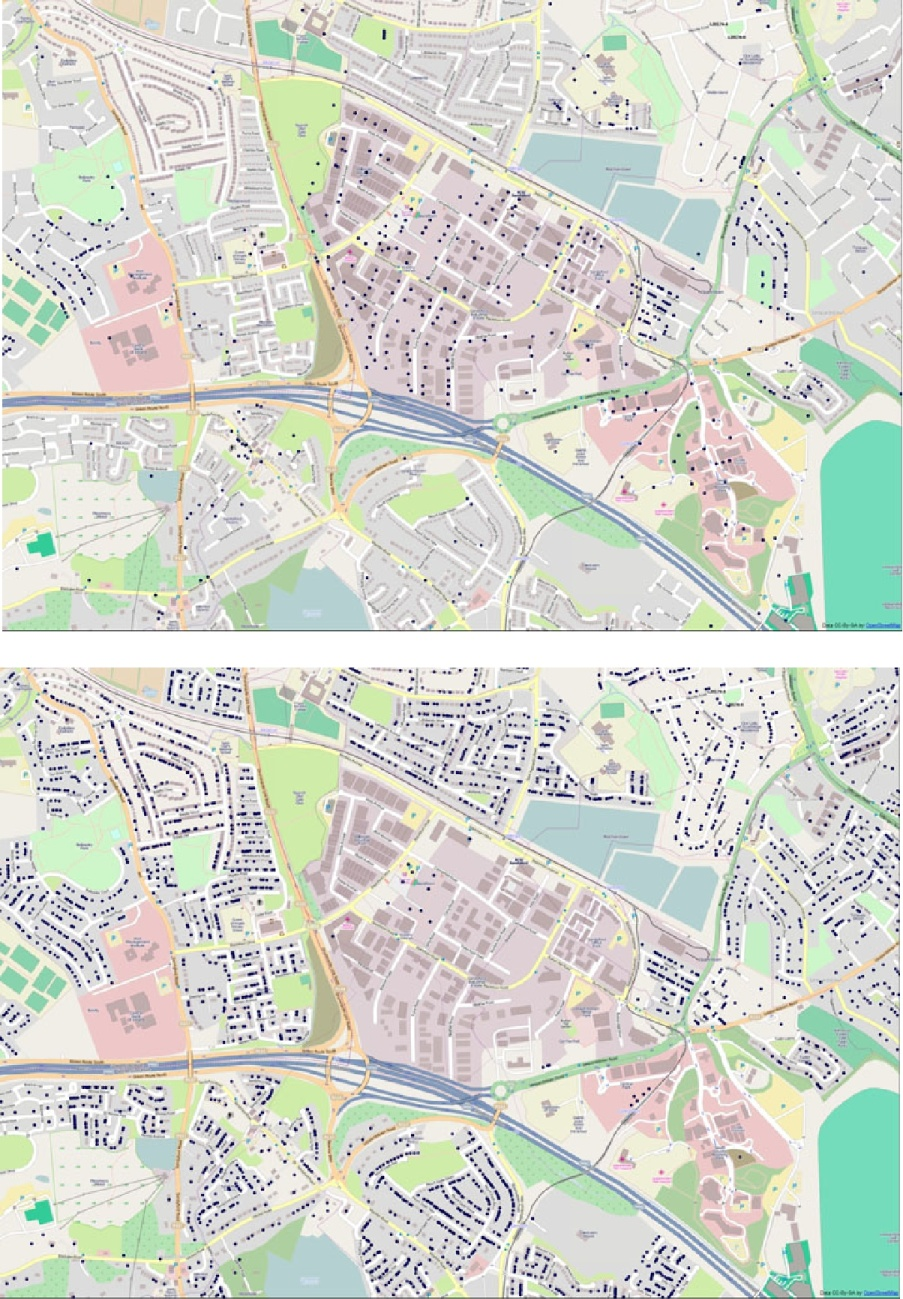
\includegraphics[width=0.99\textwidth, angle=0]{using/figures/dublin0.png}}%
{}
% ------------

% ------------
\createfigure%
{Hourly observed traffic volumes compared to the estimated traffic volumes}%
{Hourly observed traffic volumes (dashed line) compared to the estimated traffic volumes produced by \gls{matsim} using the radiation model (green line) and nearest neighbor model (orange line)}%
{\label{fig:dublin1}}%
{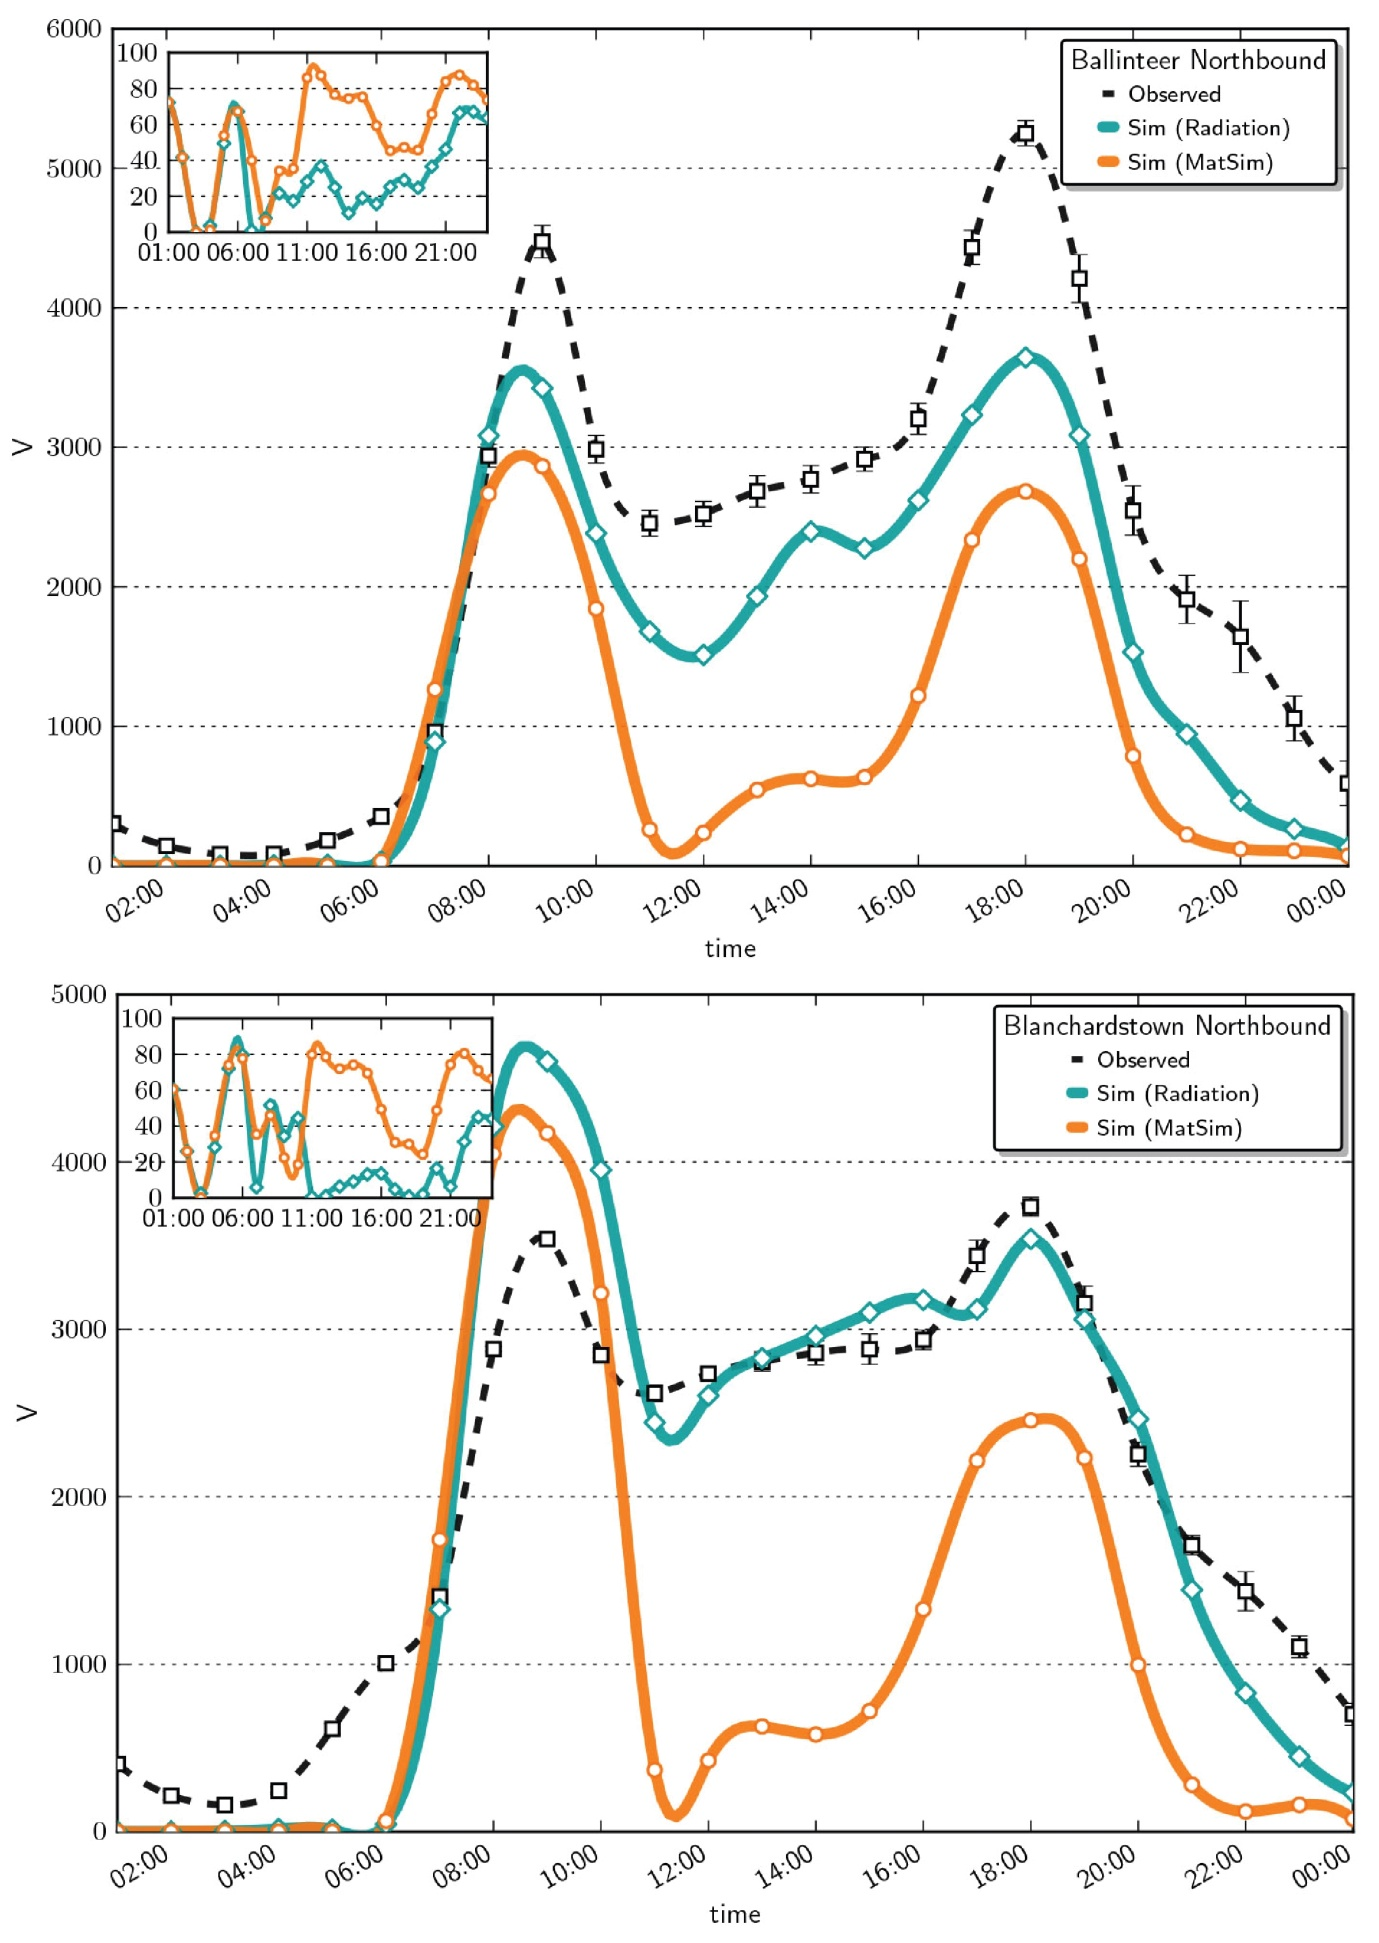
\includegraphics[width=0.99\textwidth, angle=0]{using/figures/dublin1.png}}%
{}
% ------------

% =======================================================================================





 ok

% ==================================================================================================================
% ##################################################################################################################
\section{Gauteng}
\label{sec:gauteng}
\hfill \textbf{Author:} Johan W. Joubert

\editdone{This text has undergone the professional edit. Please no grammatical changes anymore! They are most-probably wrong.}

% ##################################################################################################################
Gauteng is a landlocked province in South Africa, with  three main metropolitan areas: the city of Johannesburg, city of Tshwane (formerly Pretoria) and Eurhuleni. Although the province covers less than 3\,\% of the country's surface, it is the country's economic hub and contributes a third of the country's \gls{gdp}. The 2011~census reported a population of 12.2\,million inhabitants, a quarter of the South African population. 

The first Gauteng scenario was developed in 2008/9 and appeared in \citet[][]{Fourie2009MastersThesis} and \citet[][]{FourieJoubert_SATC_2009}. The population was synthesized from 2001 census data and travel demand was inferred from the 2003 \gls{nhts}. Initially, the network was created from a proprietary source made available for research purposes this has been replaced with a much richer \gls{osm} network.

Early comparisons already showed that the Gauteng \gls{matsim} scenario provided far more detailed results than the four-step models available at the time \citep[][]{Fourie_SATC_2010}. The scenario was also extended to include freight vehicles~\citep[][]{JoubertJEtAl_TRR_2010}.

With the introduction of an open-road tolling scheme referred to as the \gls{gfip}, the scenario was used to study the diversion patterns of different road user groups. The population was extended to included background traffic, in the form of public transport (buses and minibus taxis) and external through-traffic. This data was taken from Saturn \gls{od}-matrices made available by the sponsor, the \gls{sanral}. The impact of the tolling scheme, using vehicle-specific values of time, and a complex toll pricing regime was reported in \citet[][]{NagelKickhoeferJoubert2014HeterogeneousVoTsPROCEDIA}.

The most recent update to the synthetic population generation for the Gauteng scenario is documented on \gls{matsim}'s \url{https://matsim.atlassian.net/wiki/display/MATPUB/South+Africa} Confluence site.

% ##################################################################################################################

% ==================================================================================================================
% ##################################################################################################################
\section{London}
\label{ch:scenarios:london}
\hfill \textbf{Author:} John Serras

% ################################################################################################################## ok

% ==================================================================================================================
% ##################################################################################################################
\section{Los Angeles}
\label{ch:scenarios:losangeles}
\hfill \textbf{Author:} Michael Balmer

% ################################################################################################################## ok

% ==================================================================================================================
% ##################################################################################################################
\chapter{New York City}
\label{ch:nyc}
\hfill \textbf{Author:} Christoph Dobler

\editdone{This text has undergone the professional edit. Please no grammatical changes anymore! They are most-probably wrong.}

% ##################################################################################################################
The \gls{matsim} New York model was an example of an agent-based model based on a given activity-based demand generation process outcome: in this case, the \gls{nybpm} of Parson Brinkerhoff \citep[][]{VovshaEtAl_TRR_2002, ParsonsBrinckerhoff_ResRep_NYBPM_2005, ParsonsBrinckerhoff_ResRep_NYBPM_2009}. It produced persons with individual activity chains; \gls{matsim} was chosen as the simulation-based alternative to conventional assignment processes.

Activity locations were selected on zonal level (3\,824\,zones), timings (\ie start time and duration) were chosen using given distributions. As part of the conversion process to \gls{matsim}, locations were distributed within the zones, according to land use and buildings. For the route assignment, transport modes were converted into those supported by \gls{matsim}. The resulting population contained 5.3\,million persons (25\,\% sample).

A \gls{multimodal} network was created, containing car and public transport links, for the \gls{matsim} model. Car links were derived from the aggregated model network data, including capacity, number of lanes and speed limits. For the public transport network, a shape file containing every lines' routes was available. After converting and cleaning the data, the final \gls{multimodal} network contained 498\,000 nodes and 541\,000 links. Based on further public transport-related data, a full schedule was created, including different public transport modes (bus, train, etc.).

An example for final model outcomes was shown in Figure~\ref{fig:ny_car_share_full} and Figure~\ref{fig:ny_car_share_gross}, depicting the car share of all performed trips within a region. Red indicated a high share, blue a low. In Figure~\ref{fig:ny_car_share_full}, trips were aggregated on zonal level. In Figure~\ref{fig:ny_car_share_gross}, the \gls{matsim} model high resolution was shown; there, the trips were aggregated using hexagons with a side length of 500\,meters instead of a zonal level.

\createfigure%
{Car share (entire modeled area)}%
{Car share (entire modeled area)}%
{\label{fig:ny_car_share_full}}%
{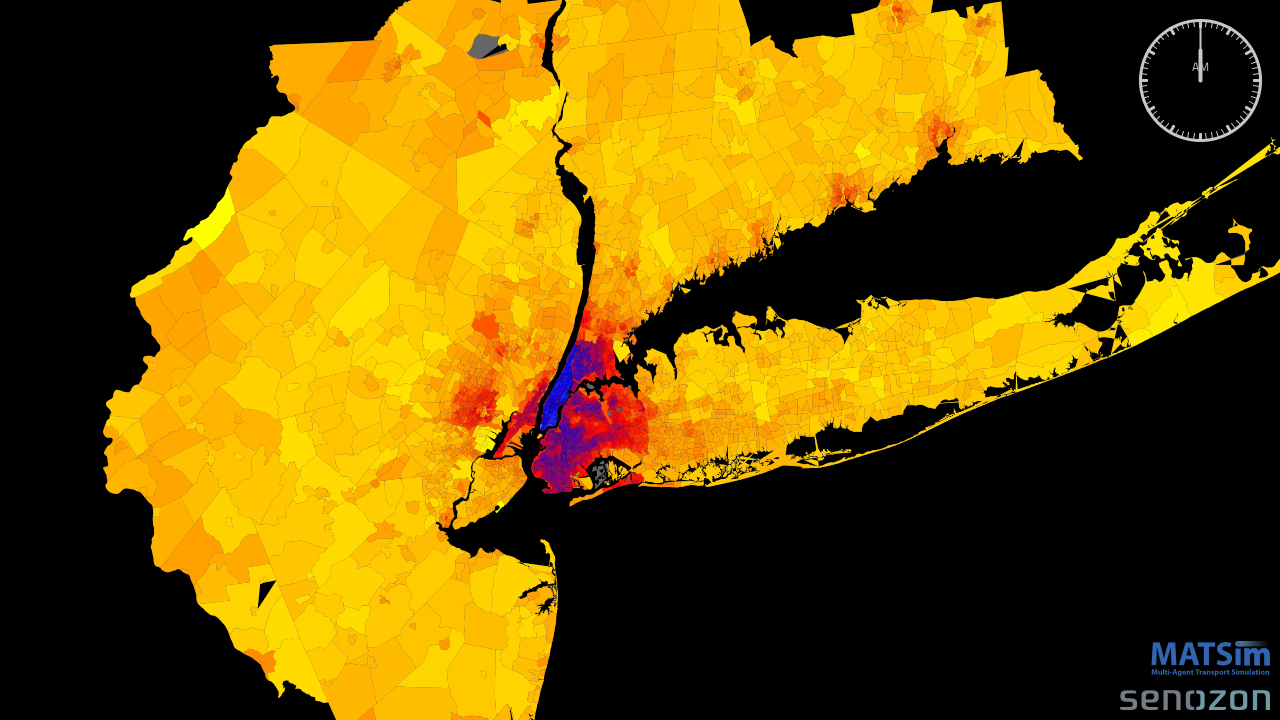
\includegraphics[width=0.95\textwidth, angle=0]{./using/figures/ny_carshare_TAZ_full.png}}%
{}

\createfigure%
{Car share (Manhattan)}%
{Car share (Manhattan)}%
{\label{fig:ny_car_share_gross}}%
{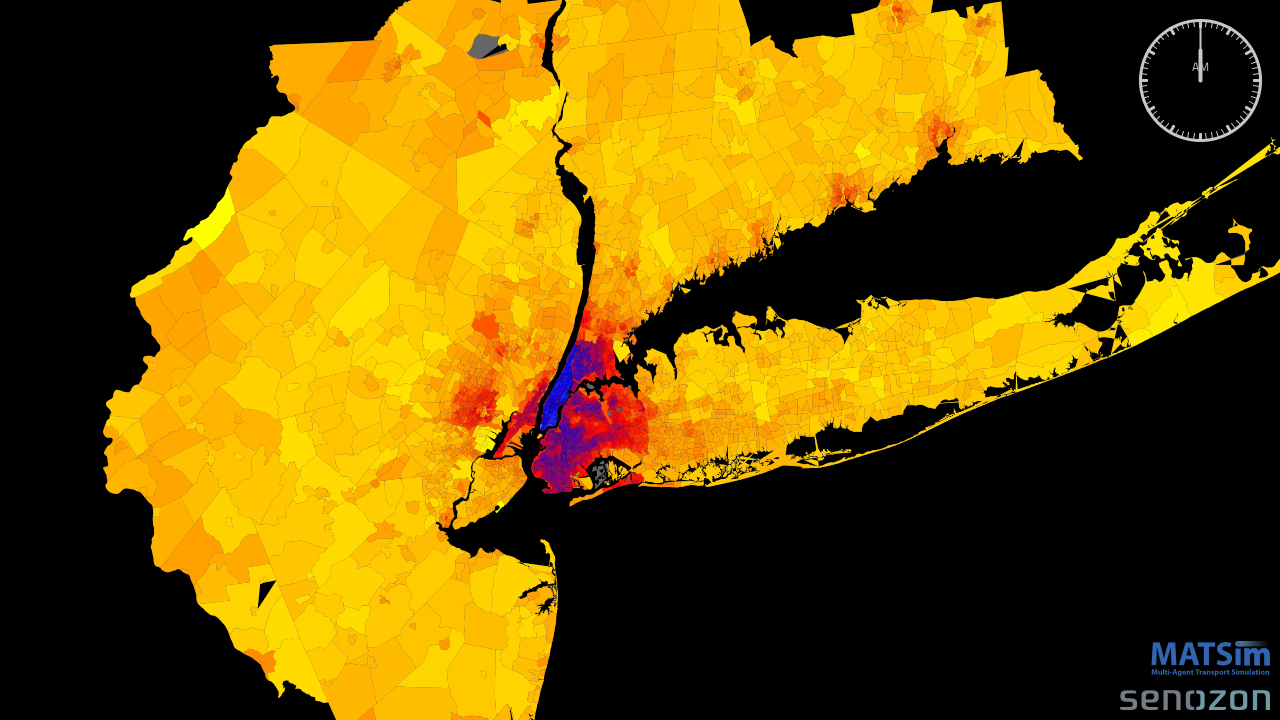
\includegraphics[width=0.95\textwidth, angle=0]{./using/figures/ny_carshare_TAZ_full.png}}%
{}

Finally, Figure~\ref{fig:ny_traffic} showed traffic flows in Lower Manhattan. Cars were represented by rectangulars, public transport vehicles by arrows. Further model outcomes were presented by \citet[][]{Balmer_unpub_ZMNY_2014}. An online movie can be found at \url{http://senozon.com/news/2014-05/zürich-meets-new-york}

\createfigure%
{Traffic flows in Lower Manhattan}%
{Traffic flows in Lower Manhattan}%
{\label{fig:ny_traffic}}%
{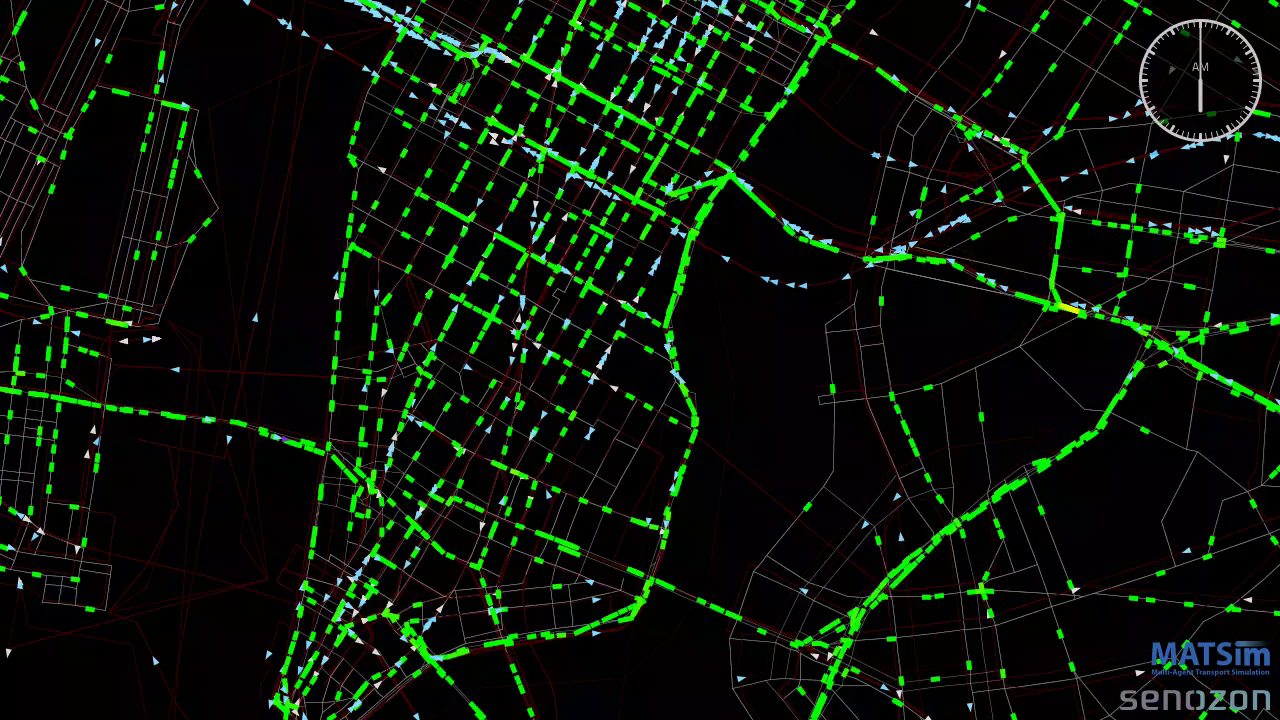
\includegraphics[width=0.95\textwidth, angle=0]{./using/figures/ny_traffic.png}}%
{}

% ################################################################################################################## ok

% ==================================================================================================================
% ##################################################################################################################
\section{Padang}
\label{sec:padang}
\hfill \textbf{Author:} Gregor Lämmel

\editdone{This text has undergone the professional edit. Please no grammatical changes anymore! They are most-probably wrong.}

% ##################################################################################################################
The Padang scenario demonstrated the \gls{matsim} application to large-scale evacuation problems. The scenario was created as part of the third party funded project, "Last-Mile". \citet{00TaubenboeckEtAl2012ConcludingLastMilePaperNatHazards} gives a comprehensive overview.
Padang is located on the west coast of Sumatra Island, Indonesia. In 2014, the city had a population of about 1\,000\,000 people. 
Because of its problematic location on the coast in a so-called "seismically locked" area~\citep{McCloskey2010Padang2009Earthquake}, Padang is prone to earthquakes and subsequent tsunamis. In the "Last-Mile" project, a realistic tsunami scenario, triggered by an earthquake about 300\,km off the coast, was identified~\citep{GosebergSchlurmann2009HazardMappingPadang}. The assumed tsunami would have left about 30\,minutes for the evacuation. The flooding would reach as far as 3\,kilometers inland, thus threatening up to 330\,000 lives. \citet{Laemmel_PhDThesis_2011} developed a \gls{matsim} scenario representing the city with its affected population. One unusual aspect of the Padang situation was the expected universal evacuation by foot; simulating pedestrians with \gls{matsim} was a novelty when this project was undertaken. The standard simulation model (see, e.g., Chapter~\ref{sec:trafficflowmodel}) was thus adapted to deal with pedestrians. 
Details were discussed in \citet{00LaemmelKluepfelNagel2009EvacPadangAtBookTimmermanns}. Another important variation, contrary to most standard transport scenarios, was that network links would flood once the tsunami reached them. Thus, accessibility---flooded or not flooded---of the network links was time-dependent, which was modeled by special time-dependent networks \citep{00LaemmelGretherNagel2009TimeDependentNetworks}. In the time-dependent network concept, link attributes---like \emph{freespeed}---could be changed, while the simulation ran, by precomputed network change events. For the Padang scenario, the network change events were extracted from microscopic flooding simulation data.

% ##################################################################################################################
%
\createfigure%
{Evacuation time analysis for downtown Padang. Numbers showing average evacuation time in minutes, which are also indicated by the colors green, yellow, red.}%
{Evacuation time analysis for downtown Padang. Numbers showing average evacuation time in minutes, which are also indicated by the colors green, yellow, red.}%
{\label{chap:using:padang}}%
{
\includegraphics[width=0.6\textwidth, angle=0]{using/figures/dwntwnpdg}}%
{}

Key Padang scenario facts:
\begin{compactitem}
\item The network consisted of about 6\,000 nodes and 17\,000 links.
\item Synthetic populations for morning, afternoon, and night were created, containing up to 330\,000 agents.
\item The flooding was modeled by a set of 109\,network change events (one per minute), affecting 7\,609 links.
\item A set of 42\,shelter buildings, which could be used for vertical evacuation, was also part of the scenario.
\end{compactitem}
Based on the Padang scenario, various evacuation strategies were investigated:
\begin{compactitem}
\item A seemingly obvious evacuation strategy was the shortest path solution, where everyone is on the shortest path. This solution, however, ignored possible congestion and led to unfeasible results:
\item The Nash equilibrium approach was better, where everyone tried to find an optimal evacuation route through iterative learning \citep{00LaemmelKluepfelNagel2009EvacPadangAtBookTimmermanns};
\item While the Nash equilibrium reduced individual evacuation time, total evacuation time might not have been minimized. The marginal social cost-based simulation approach tried to minimize total evacuation time \citep{00LaemmelFloetteroed2009KISysOptEvac,00DresslerFloetteroedLaemmelNagelSkutella2010OptimalEvacuationLargeScaleScenarios};
\item These three basic evacuation approaches were investigated together with flooding \citep{00LaemmelGretherNagel2009TimeDependentNetworks,Laemmel_PhDThesis_2011};
\item Further, an evacuation strategy to reduce exposure risk was developed by \citep{00LaemmelKluepfelNagel2010PEDRiskPrinted};
\item And finally, \citet{00FloetteroedLaemmel2010ICECShelterEvac} proposed a method to integrate shelter buildings, which are evacuation sinks (i.e.,\,safe places) 
% "\Karen{ What?? sink? Does he mean 'shed', or some kind of building? Or do the buildings have sanitary facilities? Need help with this word.}" 
with limited capacity, into the simulation.  
\end{compactitem}

% ##################################################################################################################


% ==================================================================================================================
% ##################################################################################################################
\section{Patna, India}
\label{ch:scenarios:patna}
\hfill \textbf{Author:} Amit Agarwal

% ##################################################################################################################
Patna is a medium sized city in eastern part of India. Similar to other developing nations, in Patna also, traffic conditions are heterogeneous due to presence of significantly higher number of motorized (motorbike, 14\%) and non-motorized (bike, 33\%) vehicles than car (only 2\%). Therefore, the MATSim queue simulation is modified to simulate travel demand under mixed traffic conditions.

The Patna scenario is created using household survey data from comprehensive mobility plan for Patna \citep[][]{TrippItransVks2009PatnaReport}. To create the Patna scenario, the area under Patna Municipal Corporation is used. The scenario is composed of 72 zones with a population of about 1.57 million (year 2008). In this scenario, MATSim demand is generated using trip diaries. Car, motorbike and bike are used as main congested modes. Passenger car unit for vehicles is derived using effective area occupied by vehicles. In order to allow overtaking of slower vehicles (bike) by faster vehicles (car and motorbike), preexisting, state-of-the-art FIFO (first-in-first-out) queue simulation is overridden using earliest link exit time. Detailed description of the scenario can be found in \citet[][]{AgarwalEtcMixedTraffic}.

Later, the behavior of traffic ow in modified queue simulation is analyzed by plotting fundamental diagrams and space time trajectories for car, motorbike and bike.

% ################################################################################################################## 

% ==================================================================================================================
% ##################################################################################################################
\section{Poznan}
\label{sec:poznan}
\hfill \textbf{Authors:} Michal Maciejewski, Waldemar Walerjanczyk

% ##################################################################################################################
Poznan, with its population of over 550\,000, is the fifth largest city in Poland, and together with the neighboring suburban area, it makes up an agglomeration inhabited by nearly one million people. The development of the \gls{matsim} scenario for the Poznan agglomeration began in 2012, and since then, the model has been continuously extended and improved. Currently, it is a 24-hour microscopic model of private transport. The goal is to create a 24-hour multi-agent activity-based simulation of the Poznan agglomeration, combining both private and public transport.

The road network model was extracted from \gls{osm} and includes all roads and link roads (such as entrances or exits from motorways). The final result is a high-detail road network model consisting of 17\,026 nodes and 40\,129 links. This model was calibrated in order to determine traffic flow parameters for links (e.g.,\,flow capacity, storage capacity, free-flow speed) for each of the 13\,modeled road classes \citep{PiatkowskiMaciejewski2012osmNetwork}.

The travel demand model was derived from the official trip-based 4-stage model used by the planning department of the city of Poznan; this model dates back to 2000, but since then has been frequently updated. Since the official model was originally designed for the the morning and afternoon peak hours, it had to be extended to describe travel demand throughout the day, hour after hour. As a result, the demand for private transport is represented by 24\,sets of hourly \gls{od} matrices, each set consisting of nine different matrices, one for each of nine travel motivations, namely home $\rightarrow$ work/education/shopping/other, work/education/shopping/other $\rightarrow$ home, and not related to home. This totals up to 216\,\gls{od} matrices \citep{PiatkowskiEtAl2013Poznan24hSimulation, MaciejewskiEtAl2014MikroMakro}.

The official model divides the agglomeration into less than 400\,zones, which is not sufficient for the activity locations to be accurately modeled at the microscopic level. To increase the accuracy, the \gls{osm} land use data were used. Six types of land use, namely residential, industrial, green, commercial, schools and unclassified, were used to subdivide zones into homogenous subzones. As a result, home activities were located in residential subzones, education activities at schools, shopping in residential or commercial subzones, and so on. Figure~\ref{fig:poznan_home_distribution} illustrates the distribution of \emph{home} locations when land use is taken into account \cite{PiatkowskiMaciejewski2013LandUse}.

%---------------------------------------------------------------------
\createfigure%
{Distribution of home activities based on land use}%
{Distribution of home activities based on land use}%
{\label{fig:poznan_home_distribution}}%
{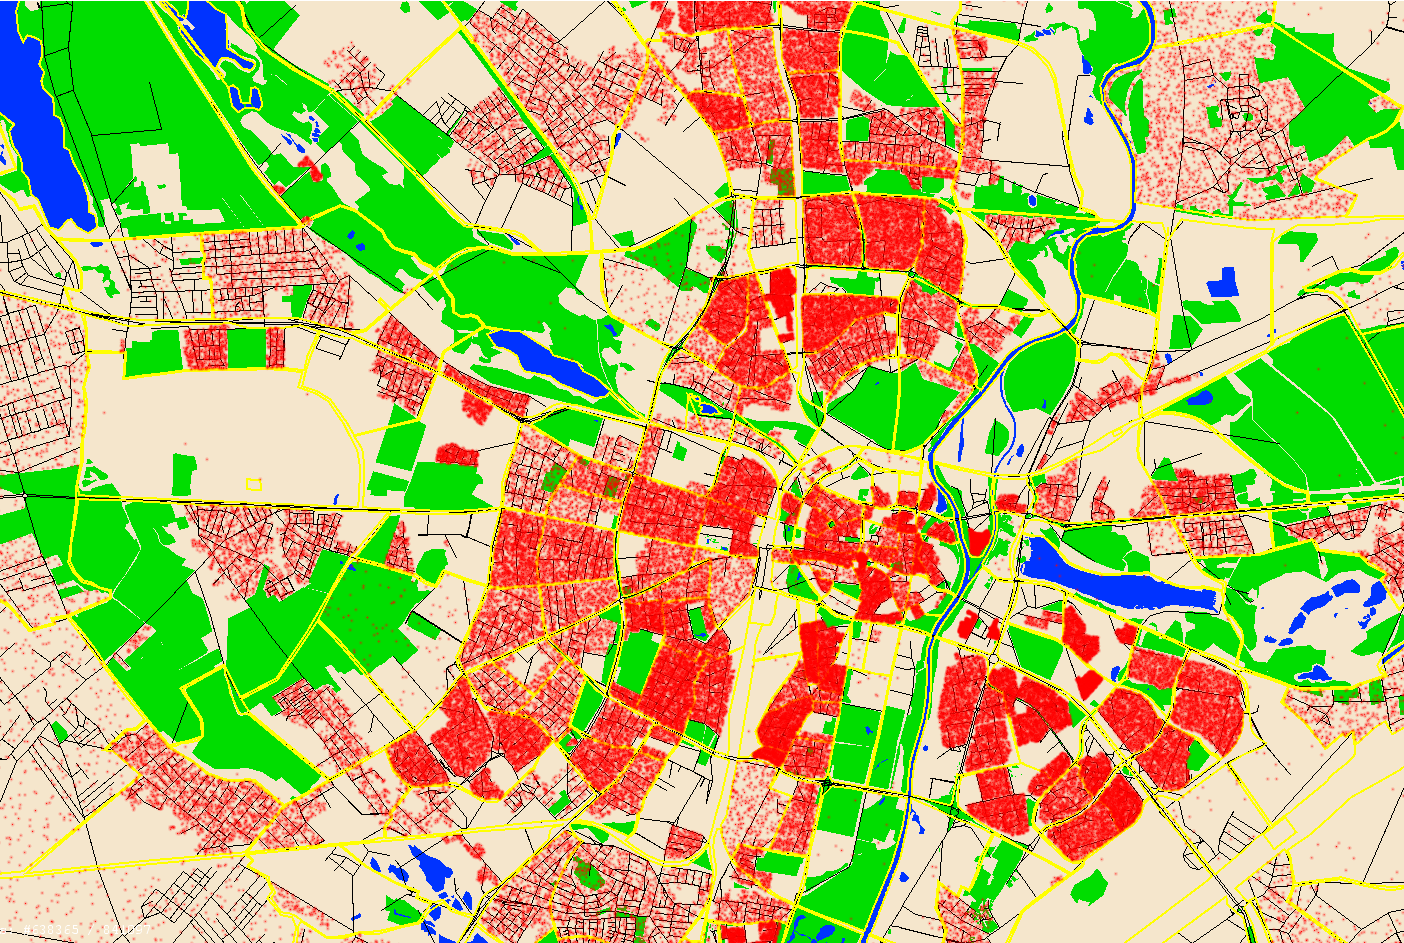
\includegraphics[width=\textwidth, angle=0]{using/figures/poznan_home_distribution}}%
{}%
%---------------------------------------------------------------------

Having calculated the \gls{od} matrices for private transport and subdivided the area into homogenous subzones, the next step was to generate the population of agents. In the first attempt, an assumption was made that each agent performs only one trip, so the number of agents equals the demand represented by the \gls{od} matrices, which is almost 840\,000. Departure times were randomly distributed (uniform distribution) over each hour, and therefore, the only decision made by each agent during the replanning phase concerned the route choice for the preselected pair of locations. The whole simulation consists of 120\,iterations, yet it usually takes about 60\,iterations to achieve a relaxed state. Figure~\ref{fig:poznan_traffic_simulation} shows the state of traffic at 7\,am.

%---------------------------------------------------------------------
\createfigure%
{Road traffic in the Poznan agglomeration at 7\,am}%
{Road traffic in the Poznan agglomeration at 7\,am}%
{\label{fig:poznan_traffic_simulation}}%
{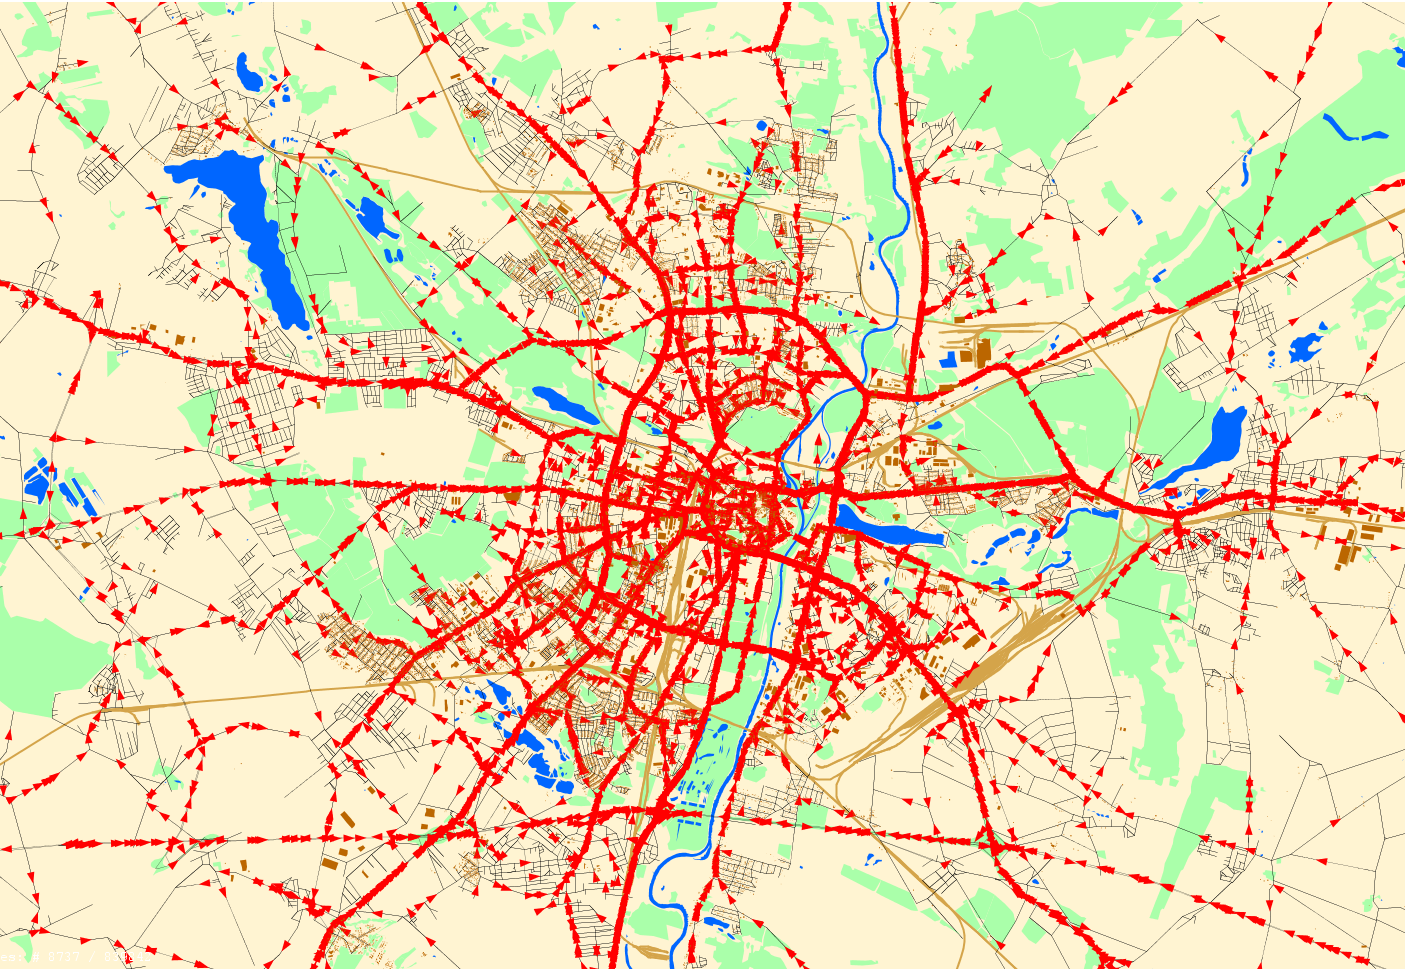
\includegraphics[width=\textwidth, angle=0]{using/figures/poznan_traffic_simulation}}%
{}%
%---------------------------------------------------------------------

Currently, the model is being updated according to a comprehensive travel study carried out in 2014. At the same time, the public transport system is being added, allowing for simulation of both private and public transport. The Poznan model has been used for simulation of real-time electric taxi dispatching, which is done by means of the \gls{dvrp} \gls{extension} (see Chapter~\ref{ch:dts}).

% ##################################################################################################################

% ==================================================================================================================
% ##################################################################################################################
\chapter{Rotterdam: Revenue Management in Public Transportation with Smart-Card Data Enabled Agent-Based Simulations}
\label{ch:rotterdam}
\hfill \textbf{Authors:} Paul Bouman, Milan Lovric

\editdone{This text has undergone the professional edit. Please no grammatical changes anymore! They are most-probably wrong.}

% ##################################################################################################################
In \citet[][]{LovricEtAl_DSS_2013} and \citet[][]{BoumanEtAl_AAMAS_2012}, we proposed two scenarios for studying public transportation revenue management via time-based pricing strategies, like peak markups and off-peak discounts, currently being used by various transit agencies. To evaluate this approach, we developed agent-based simulations using \gls{matsim} and a transportation demand generated from smart-card data collected in a Dutch urban area. In the first scenario, we simulated only a metro network, while in the second scenario we considered a \gls{multimodal} network, consisting of metro, tram and bus.%
\footnote{This research was conducted at Rotterdam School of Management and
supported by Netherlands Organisation for Scientific Research (NWO)
Complexity Grant No. 645.000.001 awarded to Dr. Ting Li and Prof.mr.dr. Peter Vervest from
Rotterdam School of Management. It was presented at \protect\gls{matsim} User Meetings in 2011 and 2012,
INFORMS International 2012 Beijing, the 7th Workshop on Agents in Traffic and Transportation at
AAMAS 2012 Valencia, Erasmus University Rotterdam, Berlin Institute of Technology, Tsinghua
University and Beijing Jiaotong University.}

In \citet[][]{LovricEtAl_DSS_2013}, we designed and implemented a decision support system for sustainable revenue management to evaluate the impact of various revenue management strategies on economic, social, and environmental performance. Figure~\ref{fig:rotterdam} shows the decision support system structure built on top of the \gls{matsim} framework. Smart card transactions (individual check-in and check-out transactions made at stations' entrance and exit gates) were used to reconstruct individual passenger's daily tours. These were inputted into \gls{matsim} as initial demand; information about the transit network and vehicle schedule was extracted from the \gls{osm} data and the public transit operator's web site, respectively. Revenue management experiments were then conducted by applying various time-based pricing strategies defined as percentage-wise discounts or markups (applied on top of the nominal price) during specific periods of the day. 

\gls{matsim}'s loop (Section~\ref{sec:inbrief}) was adapted for studying time-based pricing. First, an event handler was created to calculate whole daily tour travel fare for each individual (this was implemented using the real-life pricing scheme: a fixed fee applied at check-in, plus a variable distance-based fee applied at check-out). Second, we adapted the original Charypar-Nagel scoring function \citep[][]{CharyparNagel2005ga4acts}, by adding travel fare disutility. The existing \gls{matsim}'s time mutator was used as a replanning strategy, allowing passengers to discover more affordable travel times when pricing strategies were enforced (however, a trade-off was introduced by applying a penalty for arriving outside the expected arrival window, based on the observed smart card data check-out times).

To capture revenue management impact on the three sustainability dimensions, we added event handlers to produce a number of relevant \glspl{kpi}. The economic performance was measured by \gls{pto}, passenger kilometers revenue and vehicle load factors. Social performance was measured by seat availability (a proxy for passenger comfort), calculated from vehicle loadings after the mobility simulation. We also looked at average tour price as the measure of public transportation affordability. Impact of a pricing policy on the environment was expressed as the change in carbon footprint occurring through a demand shift between public transportation and private cars (calculated from average tour price change and demand elasticity). 

Our results showed that, by using a smart-card enabled decision support system and taking a customer-centric view, \glspl{pto} can better explore feasible solutions in a broader policy-making context that includes three dimensions of people-profit-planet sustainability. We validated our approach by comparing the simulation-generated travel fares in the nominal scenario with actual fares recorded in the smart card transactional database \citep[see][]{LovricEtAl_DSS_2013}.

To further study smart card data opportunities in demand generation, \citet[][]{BoumanEtAl_AAMAS_2012}, we introduced a pattern-based demand generation method using three different modalities' (metro, tram and bus) smart card transactions in a Netherlands urban area as input. In addition to using single day observations to generate activity-based demand, daily commuting patterns detected from longitudinal observations for a single smart card were generated. In this study, generated demands were utilized to analyze time-shifting behavior under two different revenue management policies: a plain tariff (with a fixed price per journey and a price per unit of traveled distance) and an off-peak discount. The experiment was repeated for different levels of pattern-based demand, where the varied parameter was the number of observed samples required for a smart card to be included. 

In generated demand, agents not generated using pattern-based demand had to replicate their observed tour or trip within 15\,minute windows of observed arrival and departure times. Pattern-based agents had time windows dependent on observed standard deviations in passengers' actual commuting travel patterns, which were used as a proxy for their time flexibility. This aspect of demand modeling was more detailed than \citet[][]{LovricEtAl_DSS_2013}, where agents were assumed to be homogeneous about their time flexibility. This flexibility was exploited by the time shift mutator, made available in \gls{matsim} as one of the \gls{replanning} strategies. In future work, improvements in scoring function and use of more sophisticated pattern-based demand generation approach must be considered to create more realistic scenarios for a study of time-shifting behavior under revenue management policies.

\createfigure%
{Rotterdam scenario}%
{Rotterdam scenario: Decision support system for sustainable revenue management in public transportation}%
{\label{fig:rotterdam}}%
{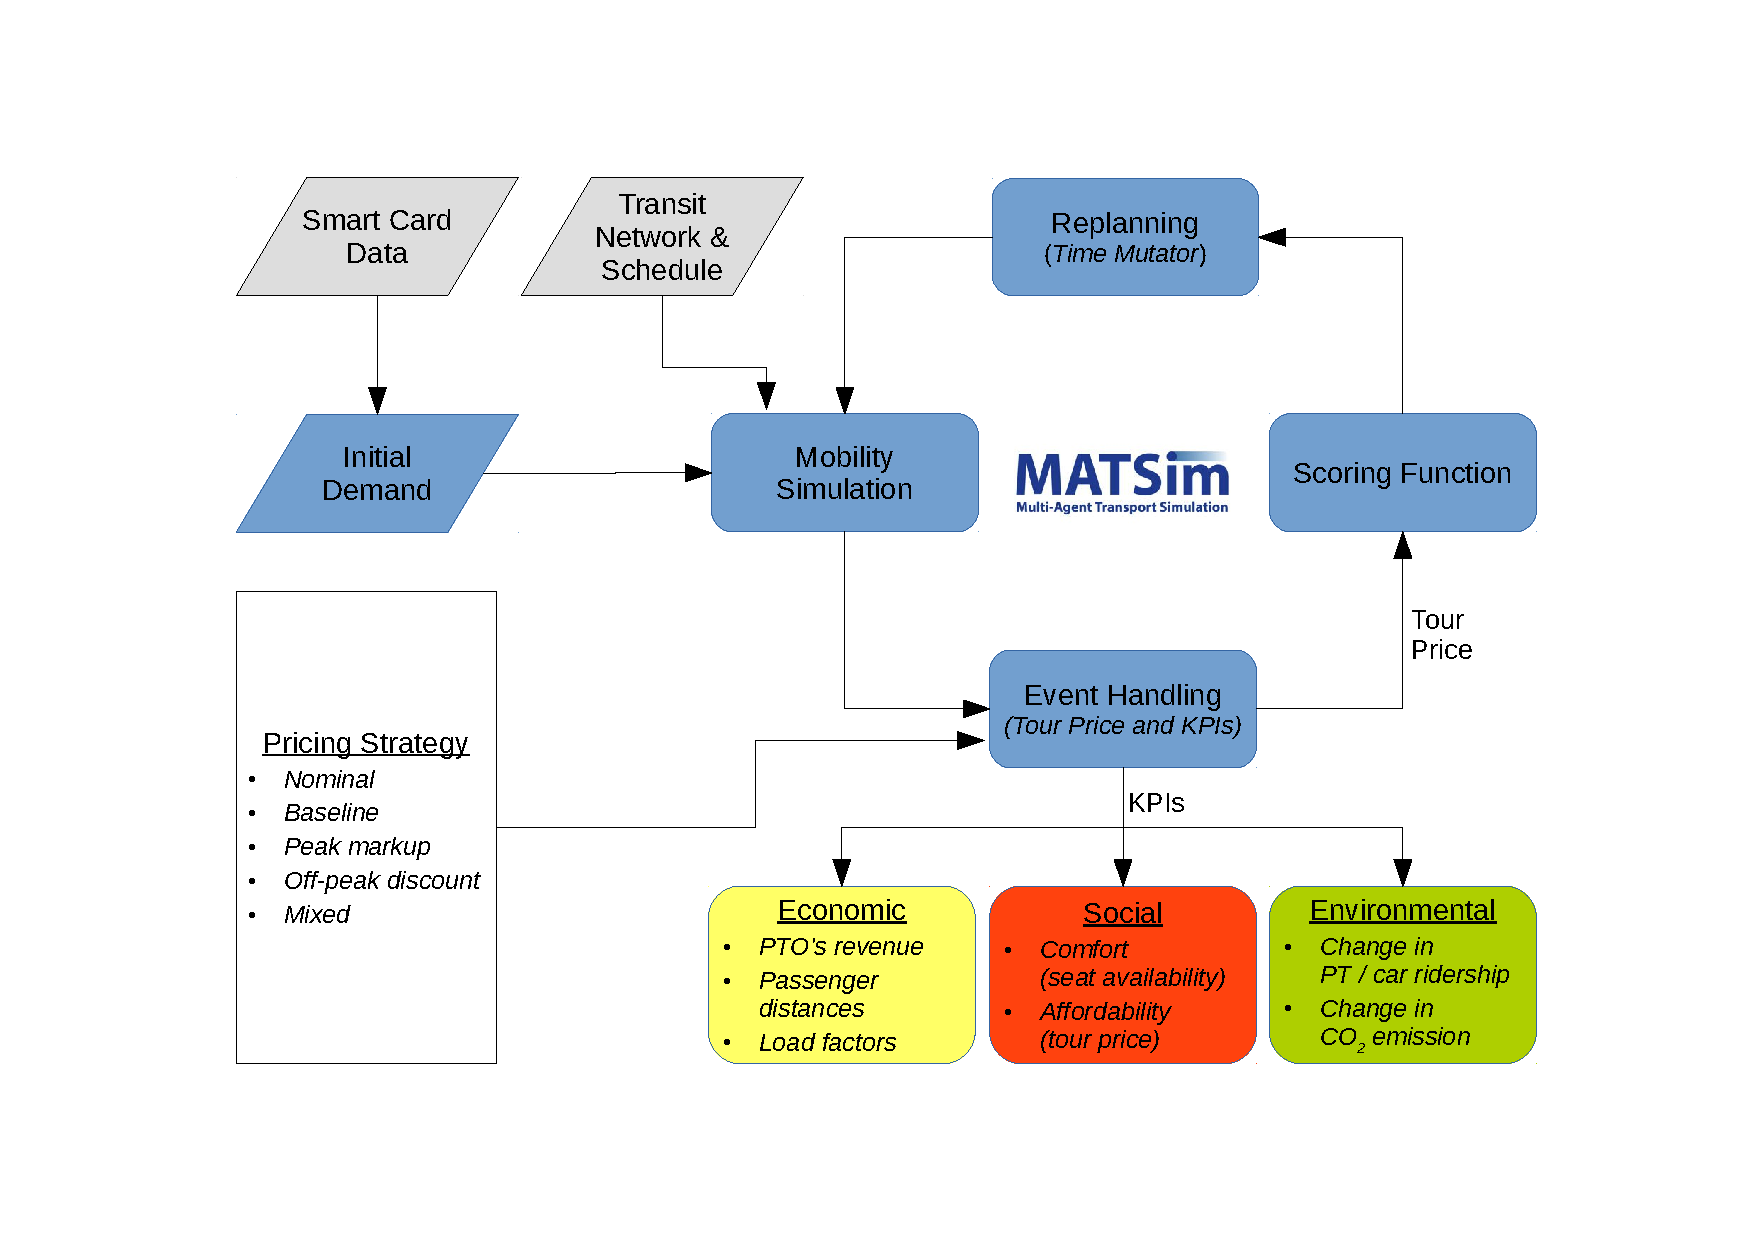
\includegraphics[width=0.85\textwidth, angle=0]{./scenarios/figures/rotterdam}}%
{}

% ##################################################################################################################

 ok

% ==================================================================================================================
% ##################################################################################################################
\section{San Francisco Bay Area}
\label{sec:sf}
\hfill \textbf{Author:} Alexey Pozdnukhov

% ################################################################################################################## ok

% ==================================================================================================================
% ##################################################################################################################
\section{Seoul}
\label{ch:seoul}
\hfill \textbf{Author:} Seungjae Lee, Atizaz Ali

% ##################################################################################################################
The MATSim model of Seoul Metropolitan was developed in 2012 as a result of long-term research collaboration between the University of Seoul (Prof. Seungjae Lee) \& ETH Zurich (Prof. Kay W. Axhausen). The model was updated on a yearly basis and the demand is generated based on 2012 Household Travel Survey Data (HHTSD). The brief statistics related to the demand (input) are summarized as follows. 

The study area covers the Seoul Metropolitan Area (Gyeonggi-do province with emphasis on Seoul Metro which comprises of 25 main administrative districts). Population Synthesizer was developed to generate the MATSim input demand based on HHTS 2012. Total population of SMA is 21.5 million; therefore, a 10\% sample was generated and simulated (2.15 million agents). A detailed network of nodes and links was generated capturing all the details (16'384 nodes and 32'768 links) for railways, highways, arterials, pedestrians, expressways and bus only lanes. EMME/2 network was converted to MATSim format. The 2012 Korean Transport Database was utilized to generate the transit schedules and vehicle definitions according to the bus types, railway and metro lines. Total number of routes is 1'317 (contains regional buses, inter-city buses, feeder line buses and metro lines etc.). In collaboration with Senozon AG, a more realistic door-door demand was generated in Seoul City in July 2014. Data source is the Korean GIS department.

In Seoul context, MATSim has been widely used for various research purposes for policy evaluation, see e.g., \citet[][]{KimEtAl_IJHE_2012, LeeAli_unpub_IWUTSCD_2014}.

A master's thesis is currently underway by this section's second author looking at transit demand generation and calibration using smart card data in SMA. The work is sequenced as follows. A video is available form the authors on request.
%
\begin{compactitem}
\item Data Mining (Trimming off non-useful data)
\item	Converting disaggregate transactions (OD’s )to individual trips and trip segments based on user ID
\item	Activities inference and assignment in SPSS database
\item	Generating transit demand (MATSim input format)
\item	Updated Transit Network \& Schedule for running the simulation
\item	Model calibration (in process)
\end{compactitem}
%
Moreover, MATSim tutorials are prepared for fall semester (2014) to help both undergrad and grad students at the Department of Transportation Engineering in getting working command at MATSim.

\createfigure%
{Seoul Scenario}%
{Seoul Scenario}%
{\label{fig:seoul}}%
{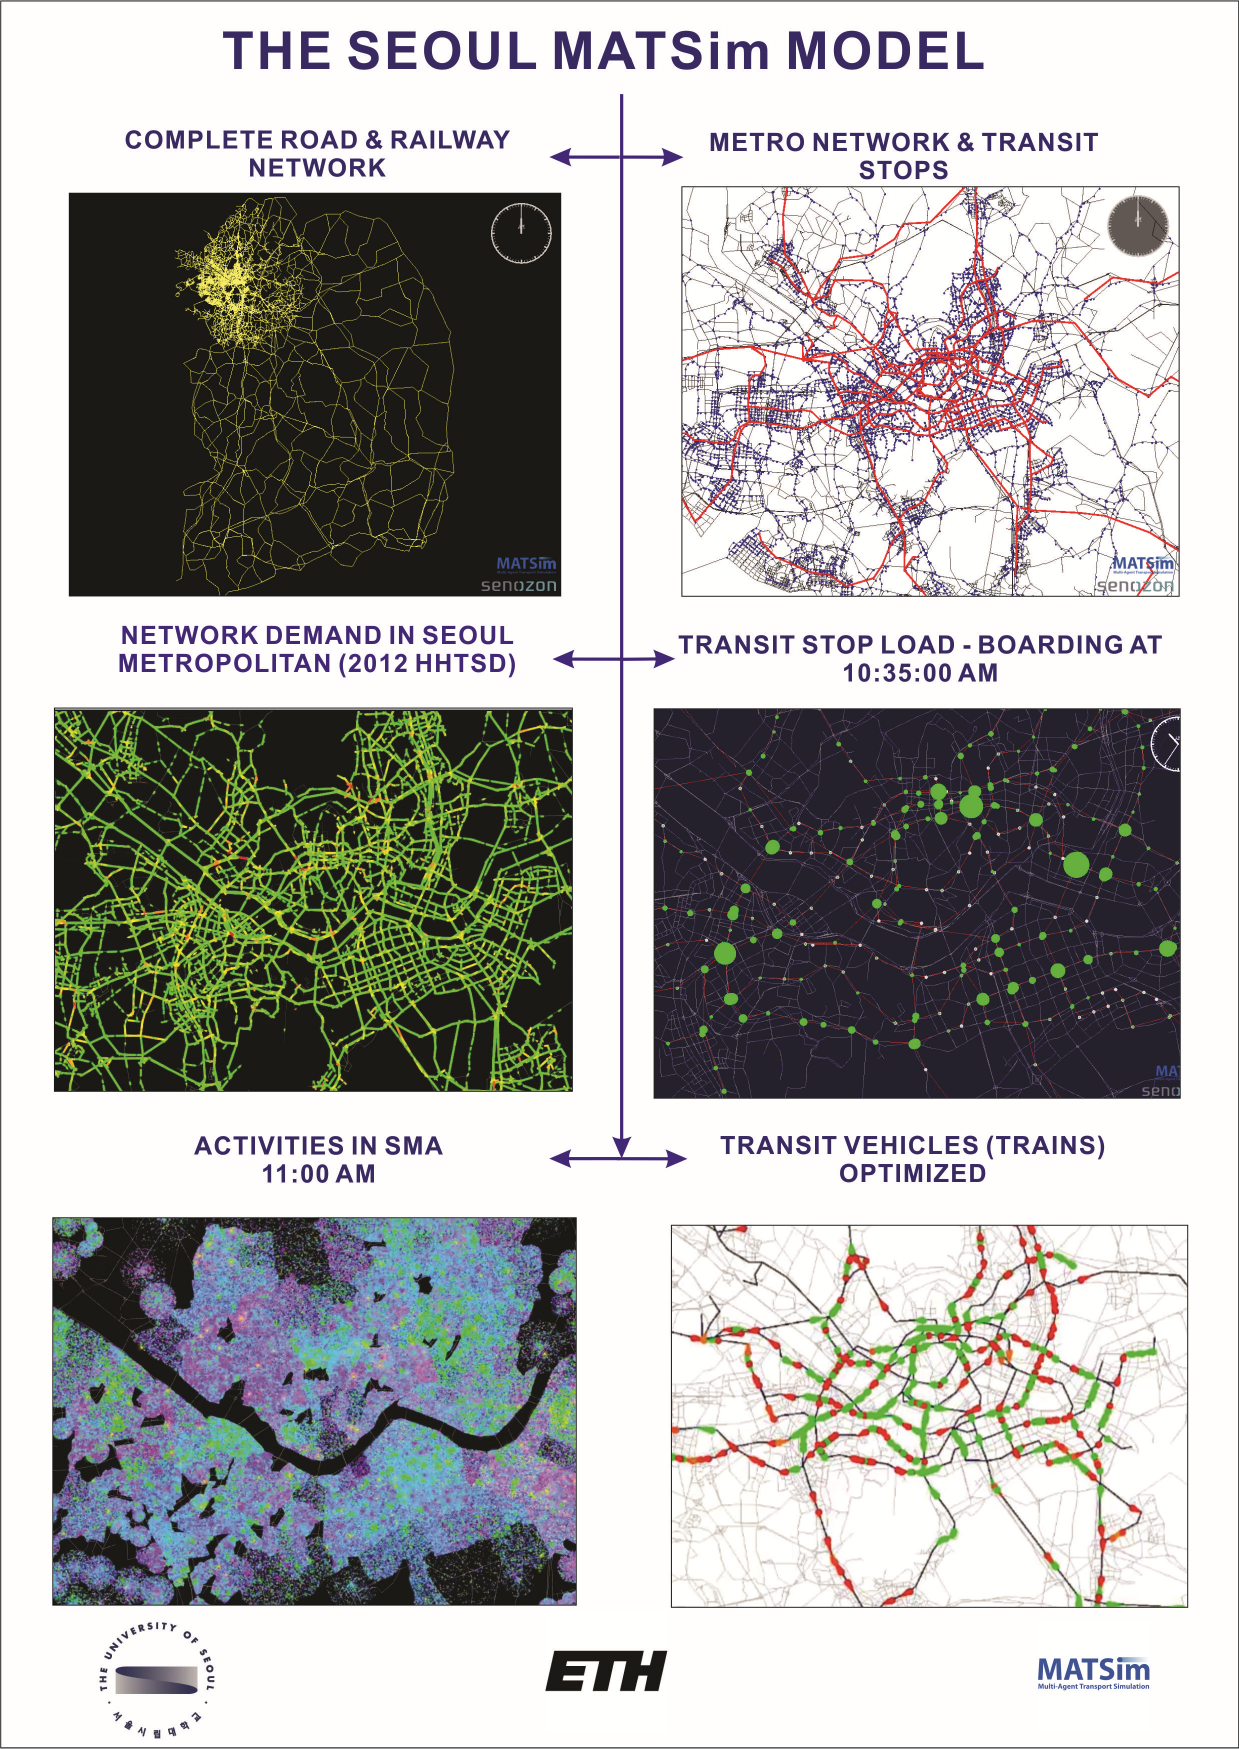
\includegraphics[width=0.99\textwidth, angle=0]{using/figures/seoul}}%
{}

% ##################################################################################################################
 
  \clearpage

% ==================================================================================================================
% ##################################################################################################################
\section{Shanghai}
\label{sec:shanghai}
\hfill \textbf{Author:} Lun Zhang

% ##################################################################################################################
Shanghai, a city of about 20\,million residential population, 6\,073\,square kilometers land area, is the biggest metropolis in China. To fully integrate the activity-based demand modeling and further public transport models, the full implementation of MATSim for Shanghai is built to forecast precise traffic demand on network as well as scientific policy evaluation. The scenario contains 200\,000\,synthetic persons and they are simulated on a network with 50\,000\,links. Key features of Shanghai scenario are as follows.

The 1\,\% sample of the actual population, about 0.2\,million agents, is used. To generate the population individual with personal attributes, MC (Monte Carlo method) are used to disaggregate available census data form the 4th Travel Survey of Residents.

The demand generation is based on 24\,hour OD matrices generated from the GPS data and synthetic population. These OD are then disaggregated into individual trips. The activity-based modeling is used to generate initial population plans by five steps: activity chain choice, duration choice, mode choice, destination choice, and route choice, in which the MNL model is used to estimate and serial choices of agents. During the simulation, activity replanning are still introduced to learn the better travel plans, while scoring for a plan is modeled by using utility-based approach.

The street network of Shanghai has been extracted from the whole OpenStreetMap network and then merged with Shanghai expressway network. Road attributes such as the number of lanes per direction or the flow capacities are set via the specification of road classifications. To simplify the original network, the optimization rules for are designed to remove the useless information that increases the computational burden.

All facilities from OD pairs are classified into the particular zones via their geographical coordinates. Three main facilities types, home, work/education and leisure, are used. The names of origin and destination facilities are obtained via reverse geocoding and these facilities are classified by their names. The resolution of facilities is hectare, in which facilities and types are randomly created according to their coordinates.

Simulated modes are as follows. A public transport system, subways and buses, is integrated with both motor traffic and non-motorized traffic. Whether individuals go to their destination public transits is base on the transit schedules. And a transport mode decision model used to make mode choice by a car or by transit is developed based on the relative utility of travel time of the two modes.

Activity replanning are used to optimize activity plans of agents and the stable state of simulation system is reached after 100\,iterations of replanning procedures. The effectiveness of the Shanghai MATSim transport simulation model is validated against the the observed counts from vehicle detectors and mode split from travel survey. Extensive simulation results indicate that most of the traffic simulation volumes match quite well with the observed counts, and the potential of MATSim for large-scale dynamic transport simulation has been demonstrated. It can provide researchers and policy makers a useful tool to evaluate traffic policies. 

The specific algorithms of integrating new data in Shanghai with MATSim inputs such as synthetic population, facilities and network are separately designed according to data characteristics. To see more detailed work about Shanghai scenario, please see the publications in \citet[][]{ZhangLEtAl_TRR_2014}.

% ################################################################################################################## \clearpage

% ==================================================================================================================
% ##################################################################################################################
\section{Stockholm}
\label{sec:stockholm}
\hfill \textbf{Author:} Joschka Bischoff

% ##################################################################################################################
The Stockholm scenario was created as a student project at TU Berlin in Summer 2014. As several groups worked on the project, the common base are a synthetic population from census data, an OSM based network and counts data.

The network is taken from OSM data in 2013. Within the city, all roads are used, whereas in outlying regions only mayor roads are part of the network.
The demand consists of home-work-home-plans only. The population sample size is, depending on the student group, between one and five percent. Agents are using car and (pseudo) public transit.

Count data for the morning peak along a mayor road, the E4, was used to calibrate the scenario. This calibration was handled differently by the groups; some just added traffic, others tried to imitate the Stockholm toll. Further documentation about the scenario is available in German language. 

% ##################################################################################################################
 ok

% ==================================================================================================================
% ##################################################################################################################
\section{Tampa}
\label{sec:tampa}
\hfill \textbf{Author:} Sashikanth Gurram

% ################################################################################################################## ok

% ==================================================================================================================
% ##################################################################################################################
\chapter{Tel Aviv}
\label{ch:telaviv}
\hfill \textbf{Author:} Christoph Dobler

\editdone{This text has undergone the professional edit. Please no grammatical changes anymore! They are most-probably wrong.}

% ##################################################################################################################
The initial Tel Aviv \gls{matsim} scenario \citep[][]{BekhorEtAl_TRB_2011} was recently extended by adding destination choice to the \gls{matsim} iterations \citep[][]{DoblerEtAl_TechRep_IVT_2014}.

The modeled area was divided into 1\,219\,\gls{taz} (Figure~\ref{fig:TAZ}); geometry was provided as a \gls{esri} shape file \citep{ESRI-ShapeFile_manual_1998}. Zonal attributes contained information on the population living in the zone, as well as types of activities that can be performed.

The population was created using population generator outcomes from the Tel Aviv activity-based model, containing socio-demographic attributes and daily schedules with up to six activities. This kept computational effort manageable; a 10\,\% population sample was simulated. Additional data was provided for external trips; for each of the three types (car, truck, commercial), \gls{od} matrices for three different time periods were available.

Network input data was taken from the \gls{emme2} model \citep[see][]{EMME_Webpage_2015}, also used by the Assignment Unit of the existing Tel Aviv Model. Conversion process details can be found in \citet{GaoWEtAl_TRR_2010}. Turning restrictions were handled by adapting the network structure, resulting in a network containing 9\,474\,nodes and 18\,570\,links (Figure~\ref{fig:network}). Some major road capacities were obviously too low (\eg noticeably lower than traffic counts indicated) and were corrected manually.

The Tel Aviv scenario contained road pricing for two arterial highways; count data for validation was available for three arterial roads.
%\karen{ Why do we have 3 here instead of the word three? I notice it has a \, after it.. is this a special notation?  thanks...}.
%
\createfigure%
{Tel Aviv scenario}%
{Tel Aviv scenario}%
{\label{fig:telavivscenario}}%
{%
  \createsubfigure%
  {\protect\gls{taz}}%
  {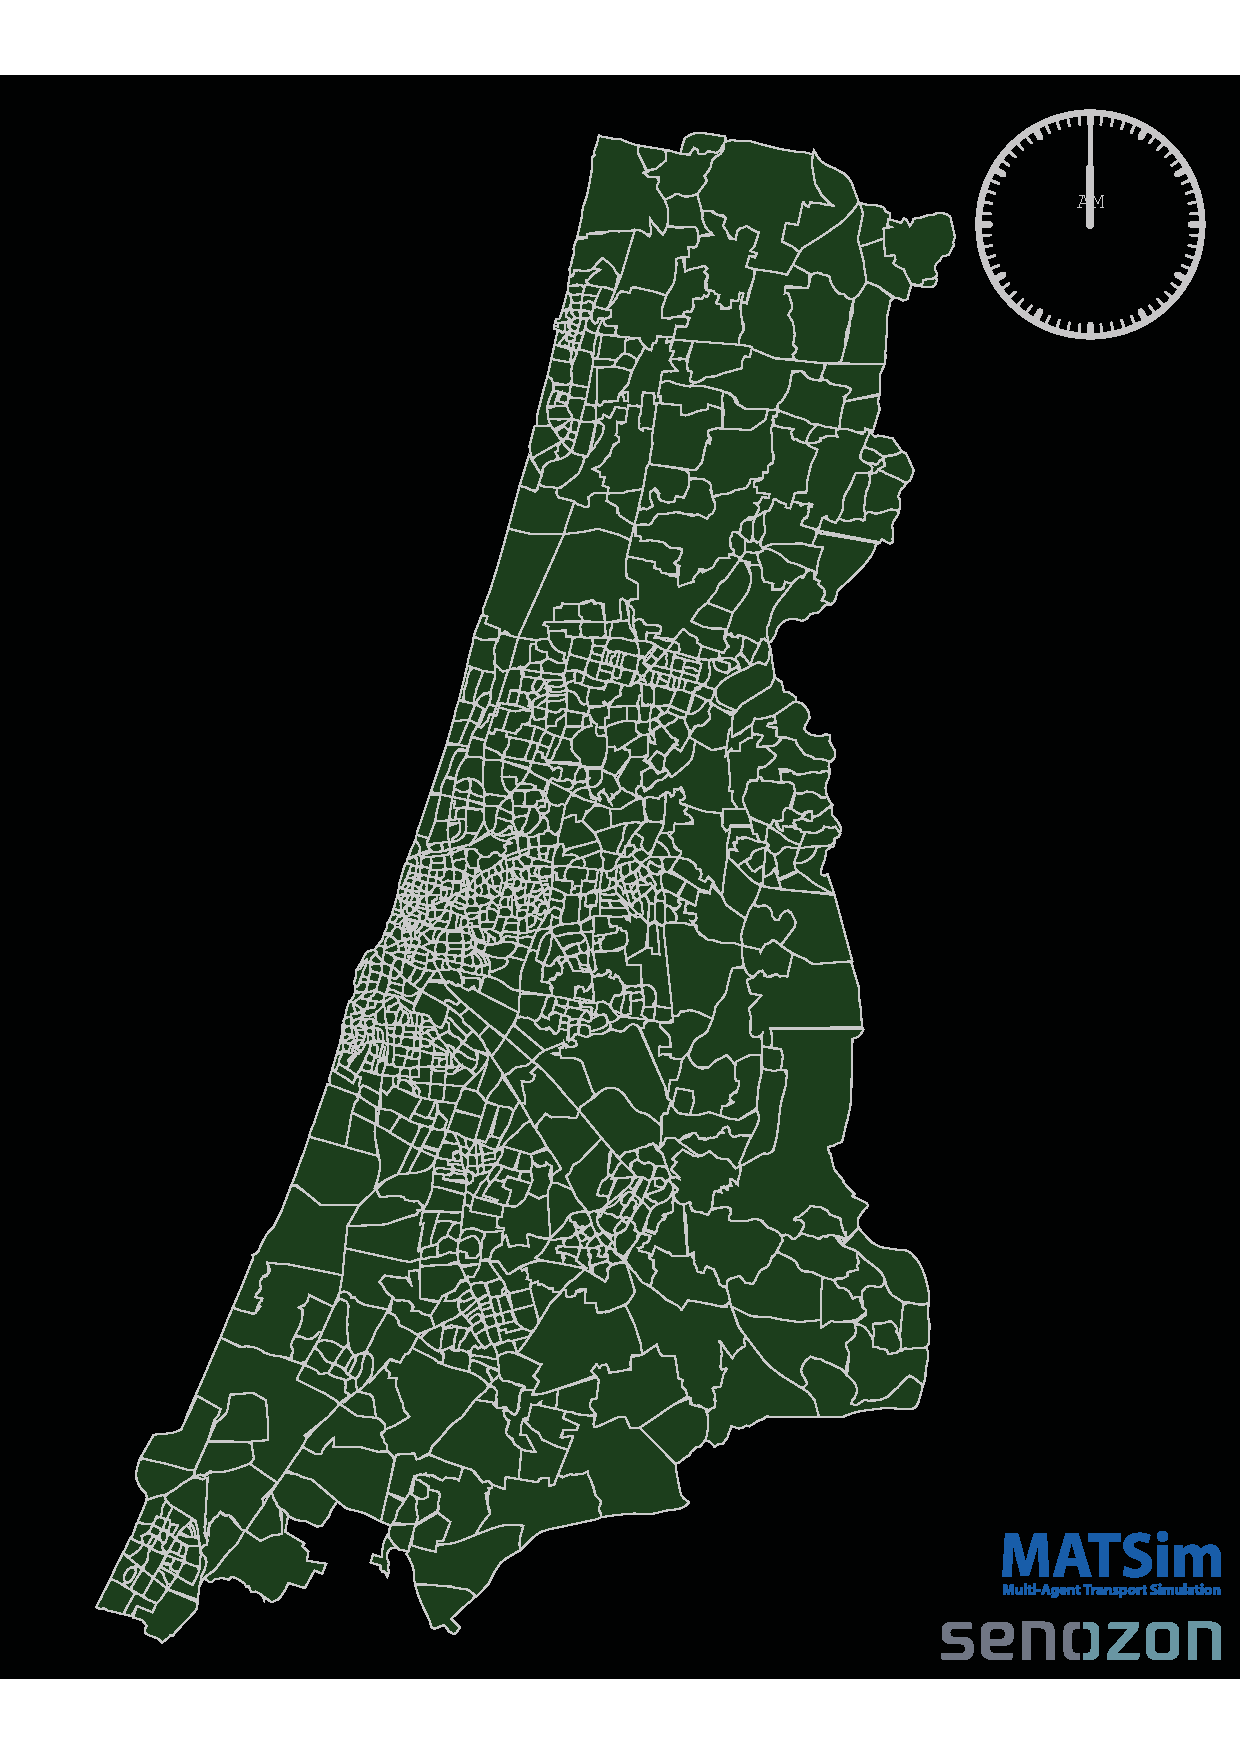
\includegraphics[width=0.49\textwidth,angle=0]{scenarios/figures/TelAviv_TAZ}}%
  {\label{fig:TAZ}}%
  {}%
  \createsubfigure%
  {Network}%
	{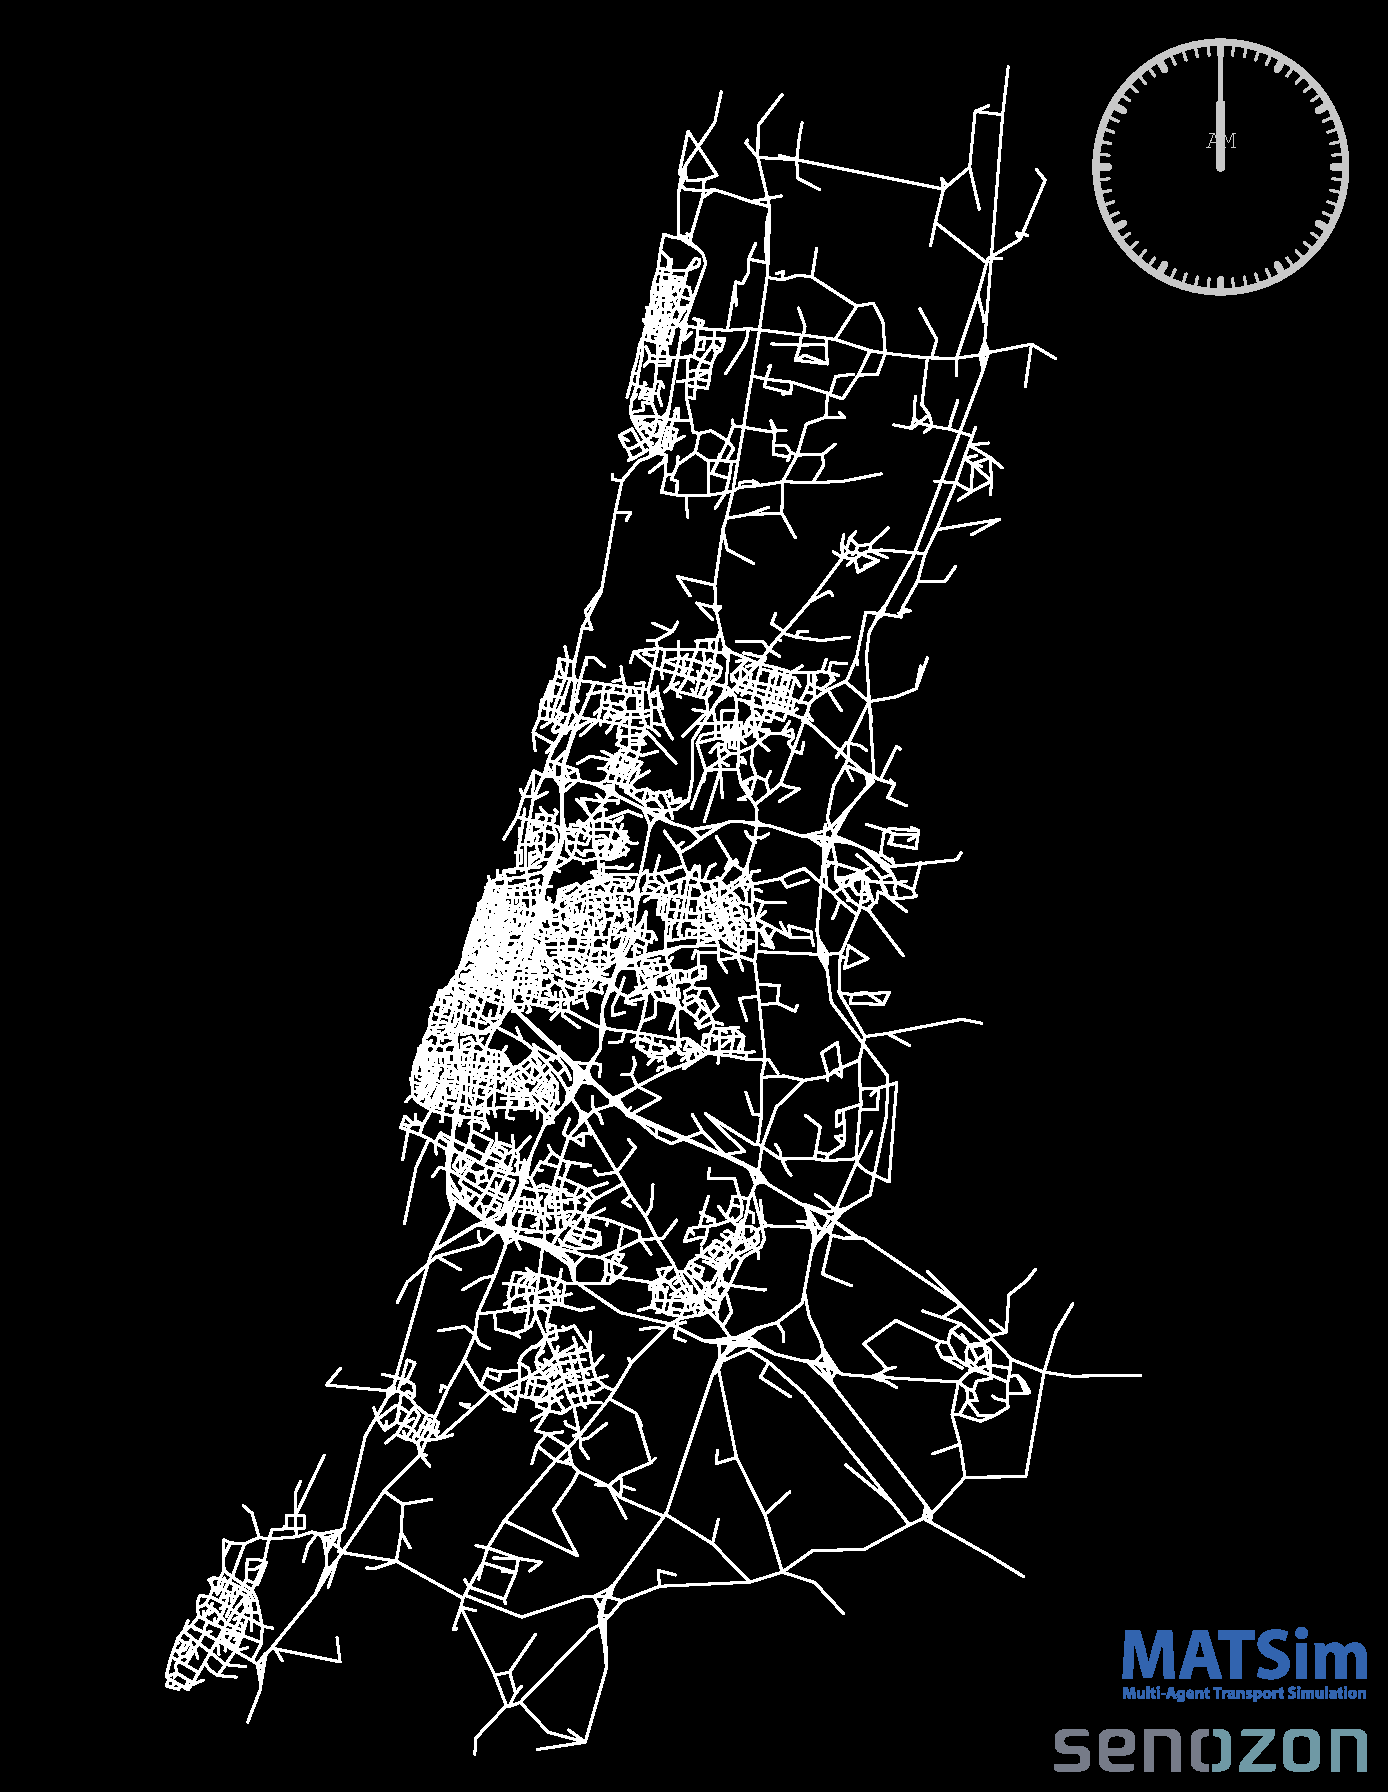
\includegraphics[width=0.49\textwidth,angle=0]{scenarios/figures/TelAviv_RoadNetwork}}%
  {\label{fig:network}}%
  {}%
}%
{}

% ##################################################################################################################
 \clearpage

% ==================================================================================================================
% ##################################################################################################################
\section{Toronto}
\label{sec:toronto}
\hfill \textbf{Author:} Adam Weiss, Peter Kucireck, Khandker Nurul Habib

% ##################################################################################################################
\subsection{Study Area:}
The Greater Toronto and Hamilton Area (GTHA) is situated to the north west of Lake Ontario in the province of Ontario, forming Canada’s largest urban region. The GTHA’s current population is over 6.5 million, with projected growth to approximately 8.6 million by 2031. 

% =============================================================================================
\subsection{Population, Demand Generation and Activity locations}
The Transportation Tomorrow Survey (TTS) forms the basis of the travel demand to be used for the multimodal assignment simulation. The TTS is a retrospective telephone survey conducted in the GTHA every 5 years. The TTS samples just over 5\% of the GTHA households. The survey collects household socioeconomic and geographical characteristics, characteristics of each household member, and a full 24 h travel diary for each household member. The current MATSIM models use the TTS travel diary records to generate the plans file. There has also been some investigation into the integration of the Travel Activity Scheduler for Household Agents (TASHA) activity based model, which has been developed for the GTHA. Irrespective of the source of the demand data, both sources provide the traffic zone location of all activities. The Toronto implementation will then randomly distribute the activities around the traffic zone, resulting in unique x-y coordinates for each activity. Within the current implementation of MATSIM within Toronto, no development of MATSIM facilities has been attempted.

% =============================================================================================
\subsection{Network Development and Simulated Modes}  
The GTHA MATSIM implementation uses a preexisting planning level network for static user equilibrium assignment using the EMME traffic assignment software. This network is converted to a MATSIM network using a conversion tool, which can be found in the MATSIM Toronto playground. More recently, this network was merged with GTFS data for 5 of the 8 major regional transit agencies to allow for multimodal demand assignment.  

% =============================================================================================
\subsection{Calibration, Validation, Results}
The Toronto MATSIM implementation has been compared to the more conventional large-scale assignment models with varying degrees of success. While the work of \citet[][]{GaoWEtAl_TRR_2010}, found that travel time, travel distance, link flows and speeds were all reasonably comparable and in fact more plausible than those achieved through the EMME assignment. Conversely, work on transit assignment done first by \citet[][]{Kucirek_MastersThesis_2012} and then by \citet[][]{WeissEtAl_CJCE_2012} found that there were limitations associated with predicting line boardings based on different transit technologies and agencies, which utilized different fare structure, suggesting that further work to calibrate the multimodal assignment model is required. These issues are exasperated by the current implementations inability to distinguish between in vehicle dwell times and out of vehicle wait times, which ideally should be weighted differently, particularly given the climate and prominence of outdoor bus stops within the region. 

% =============================================================================================

% ################################################################################################################## ok

% ==================================================================================================================
% ##################################################################################################################
\section{Trondheim}
\label{sec:trondheim}
\hfill \textbf{Authors:} Stefan Flügel, Julia Kern, Frederik Bockemühl

\editdone{This text has undergone the professional edit. Please no grammatical changes anymore! They are most-probably wrong.}

% ##################################################################################################################
The Institute of Transport Economics (TØI), in cooperation with Julia Kern from TU-Berlin and Frederik Bockemühl from Hasselts University, built a first prototype model for the region of Trondheim (Norway) \citep[][]{FluegelKern_unpub_WTS_2014}.

The road network data was imported from a publicly accessible data base (Elveg). Figure~\ref{fig:trondheimnetwork} illustrates the network. 
%
\createfigure%
{Network and simulated traffic in Trondheim and surroundings}%
{Network and simulated traffic in Trondheim and surroundings for 6:55\,am \citep[source][]{FluegelEtAl_Samferdsel_2014}}%
{\label{fig:trondheimnetwork}}%
{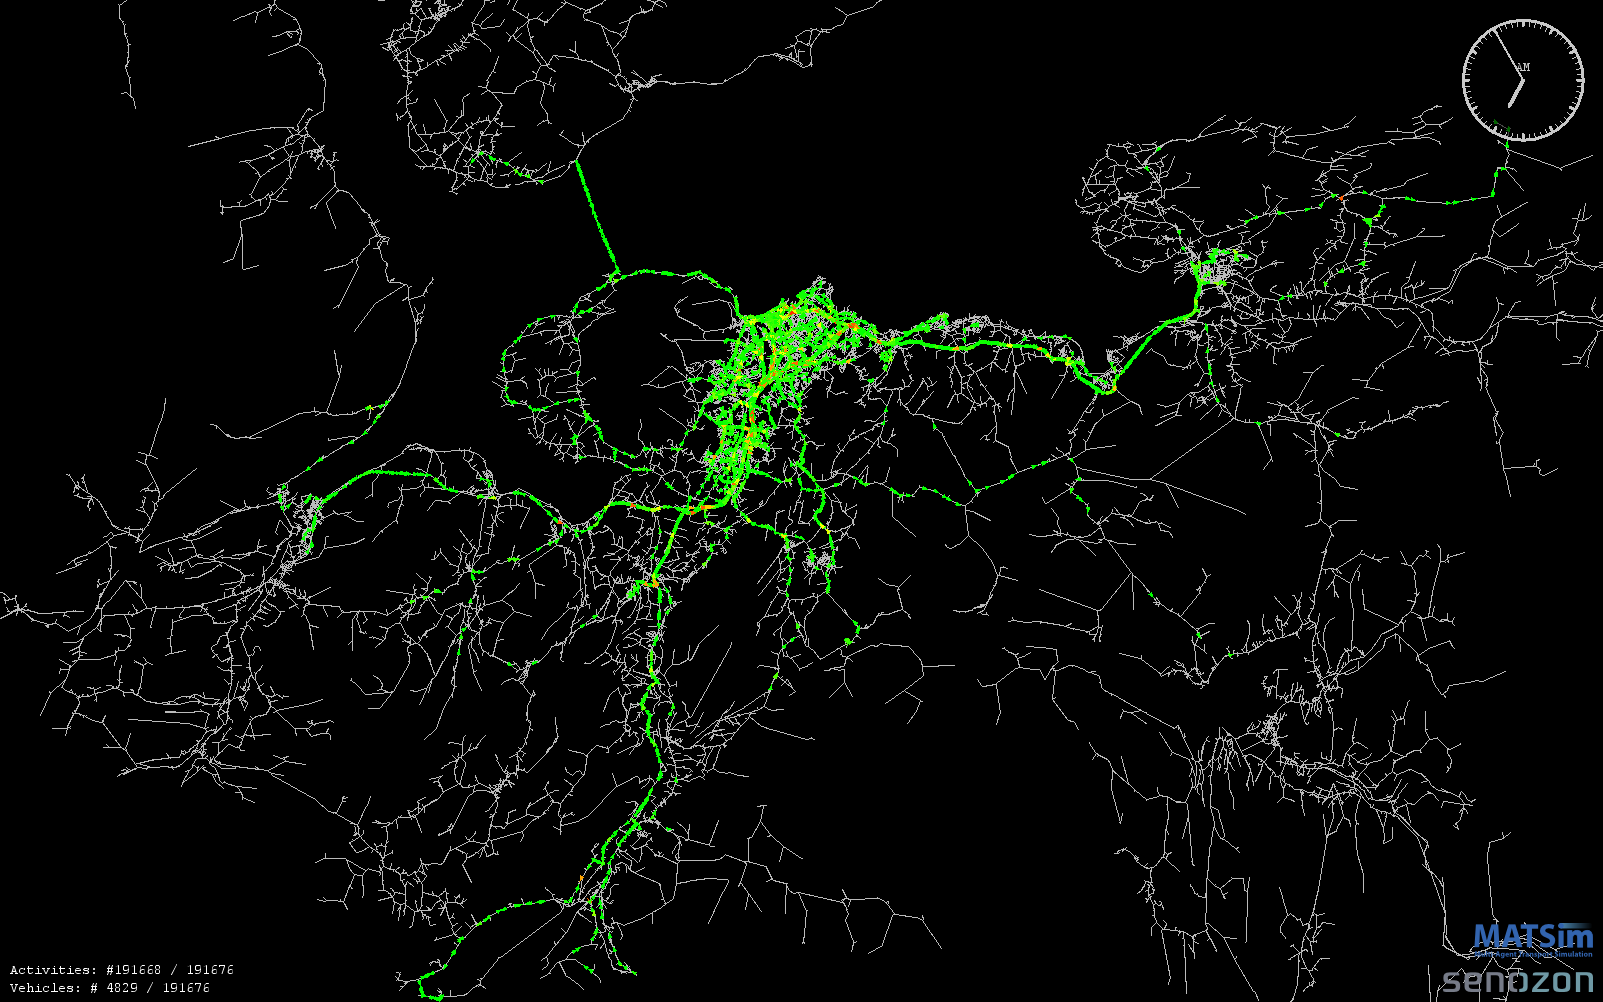
\includegraphics[width=0.85\textwidth, angle=0]{./using/figures/trondheimnetwork.png}}%
{}
%
Most required link information could be directly inferred from the data base. The lane capacity (vehicles per hour) was assumed to be a flat 1\,800 per lane. Existing toll stations, with their current toll structures, were coded manually in the network file. The public transport, walk and cycle networks had not been implemented at this time. Agents using one of these modes were teleported; travel times were calculated with predefined speeds per transport mode. 
Initial demand was derived from the National Travel Survey (NTS 2009) travel diaries. 4\,453 respondents were simply scaled up to 191\,676 agents; activity locations and departure times were slightly randomized to avoid clusters. This model differentiated only between work and ``other'' activities. Desirable working hours were specified as 8\,hours; demand consisted only of private cars (no trucks). 

Standard utility functions were applied, but in the calibration process, default values for travel time disutility in different transport modes were adjusted so that the model would reproduce observed market shares. The simulated traffic fit (in the reference scenario) against real-world counts was deemed satisfactory for a first implementation \citep[][]{Bockemuehl_TechRep_UH_2014}. 

Standard behavioral modules in \gls{matsim} were included in the Trondheim model. Agent could react to policy measures through three choice dimensions: changing route, changing transport mode and changing departure time. To test whether \gls{matsim} predicted reasonable behavioral changes, a small case study was performed. Additional tolls on streets (bridges and tunnels) to Trondheim city center were coded in the network and three congestion price structure were tested. Figure~\ref{fig:loadcurve} illustrates the effects on the simulated cars entering and leaving Trondheim city center. 
%
\createfigure%
{Cars entering/leaving Trondheim city center}%
{Cars entering/leaving Trondheim city center in reference scenario and three congestion pricing scenarios \citep[source][]{Bockemuehl_TechRep_UH_2014}}%
{\label{fig:loadcurve}}%
{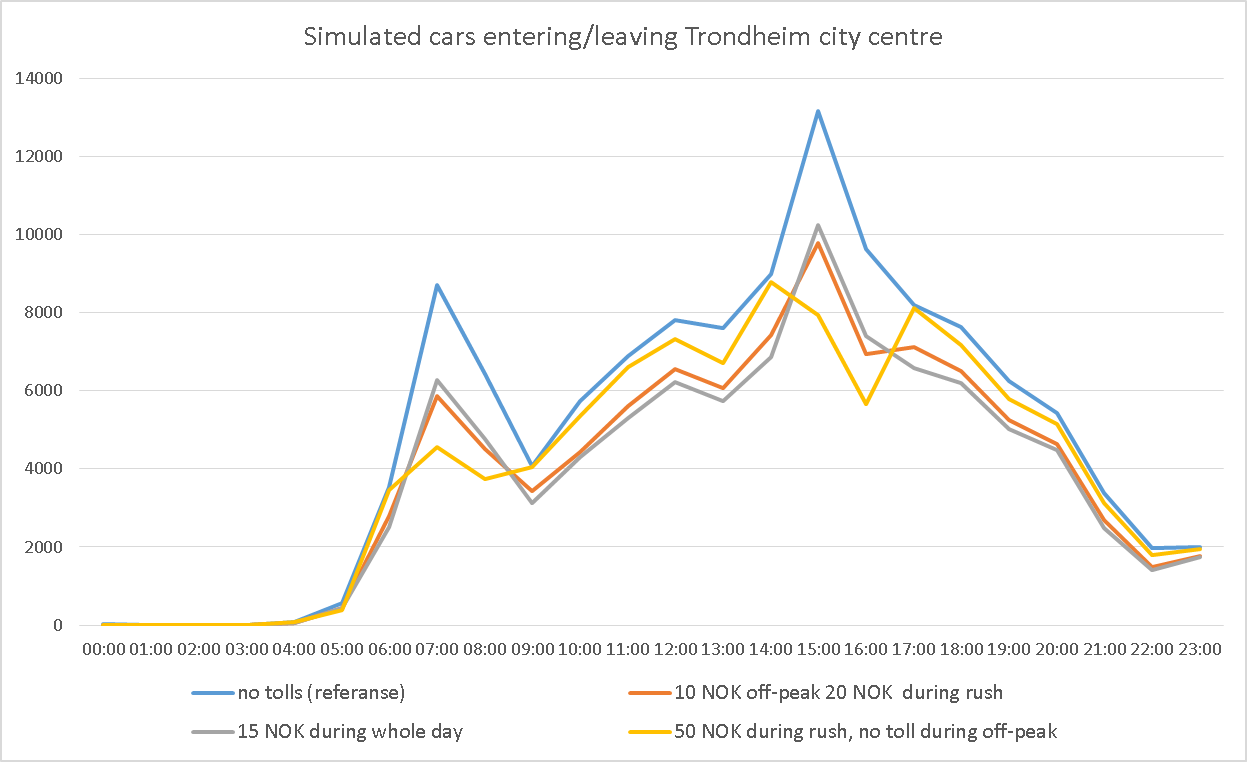
\includegraphics[width=0.85\textwidth, angle=0]{./using/figures/trondheimloadcurve.png}}%
{}
%
Compared to the reference scenario without tolls, total number of cars was reduced in all toll scenarios. Some agents changed transport modes; others, who would have driven through Trondheim center, changed their route. Comparing the three different congestion-pricing structures, it was also evident that agents changed departure time. The difference between the 15\,\glspl{nok} flat scenario and the 10/20\,\glspl{nok} scenario was small; the effect in the 50\,\glspl{nok} rush scenario was substantial. Actually, in this scenario, traffic was heavier before 3\,pm and after 5\,pm implying that many agents changed departure time to avoid high congestion pricing.  

% ##################################################################################################################   










 \clearpage

% ==================================================================================================================
\section{Yarrawonga and Mulwala: Demand-Responsive Transportation in Regional Victoria, Australia}
\label{sec:yarrawonga}
\hfill \textbf{Author:} Nicole Ronald

% ==================================================================================================================
In November 2013, Public Transport Victoria (PTV) implemented a service called
Flexiride in twin towns in regional Victoria, consisting of an on-demand public
transport service using taxis. This service replaced an existing fixed-route bus
service, which had a low patronage.
%\ah{I replace PTV everywhere by its full name as PTV is so prominent with VISUM}

The aim of this scenario was to investigate the change in operational
performance between two different \gls{drt} schemes: the Flexiride scheme and a
completely ad-hoc scheme. More details can be found in
\citep[][]{RonThoWin2015}. This work is a first step towards developing a
decision-support tool to evaluate different \gls{drt} schemes, in particular
integrated with other modes of transport. 

% --------
%Associated projects: 
The scenario was built as part of a larger project exploring the viability of
mobility-on-demand, focusing on ridesharing and \gls{drt} services \citep[][]{Ronald_iMoD_2014}.

% --------
%Study area: 
The scenario covers twin towns on the border of Victoria and New South Wales,
Australia, separated by the Murray River. Yarrawonga (Victoria) has a population
of 7\,057 and an area of 95.0\,square kilometers, while Mulwala (New South Wales) has a
population of 1\,904 and an area of 18.6\,square kilometers. 

The Flexiride scheme delivers six services on weekdays and three services on
Saturday, leaving the center of Yarrawonga (Orr St) at fixed times. The local
taxi operator is paid a holding fee by Public Transport Victoria to ensure that a taxi is available at
Orr St at the nominated time. The taxi returns to normal service if there are no
bookings and no passengers waiting.

Passengers can ride either by booking over the phone at least 10\,minutes before
the service is scheduled to depart from Orr St, or by arriving at Orr St in
person to begin their trip. Existing bus stops were used as pickup and dropoff
points.

Figure~\ref{fig:yarrawonga} shows the stops in both towns; the main stop in Yarrawonga, Orr St, is denoted by a star.
%
\createfigure%
{Location of bus stops in Yarrawonga/Mulwala}%
{Location of bus stops in Yarrawonga/Mulwala, including \gls{od} zones}%
{\label{fig:yarrawonga}}%
{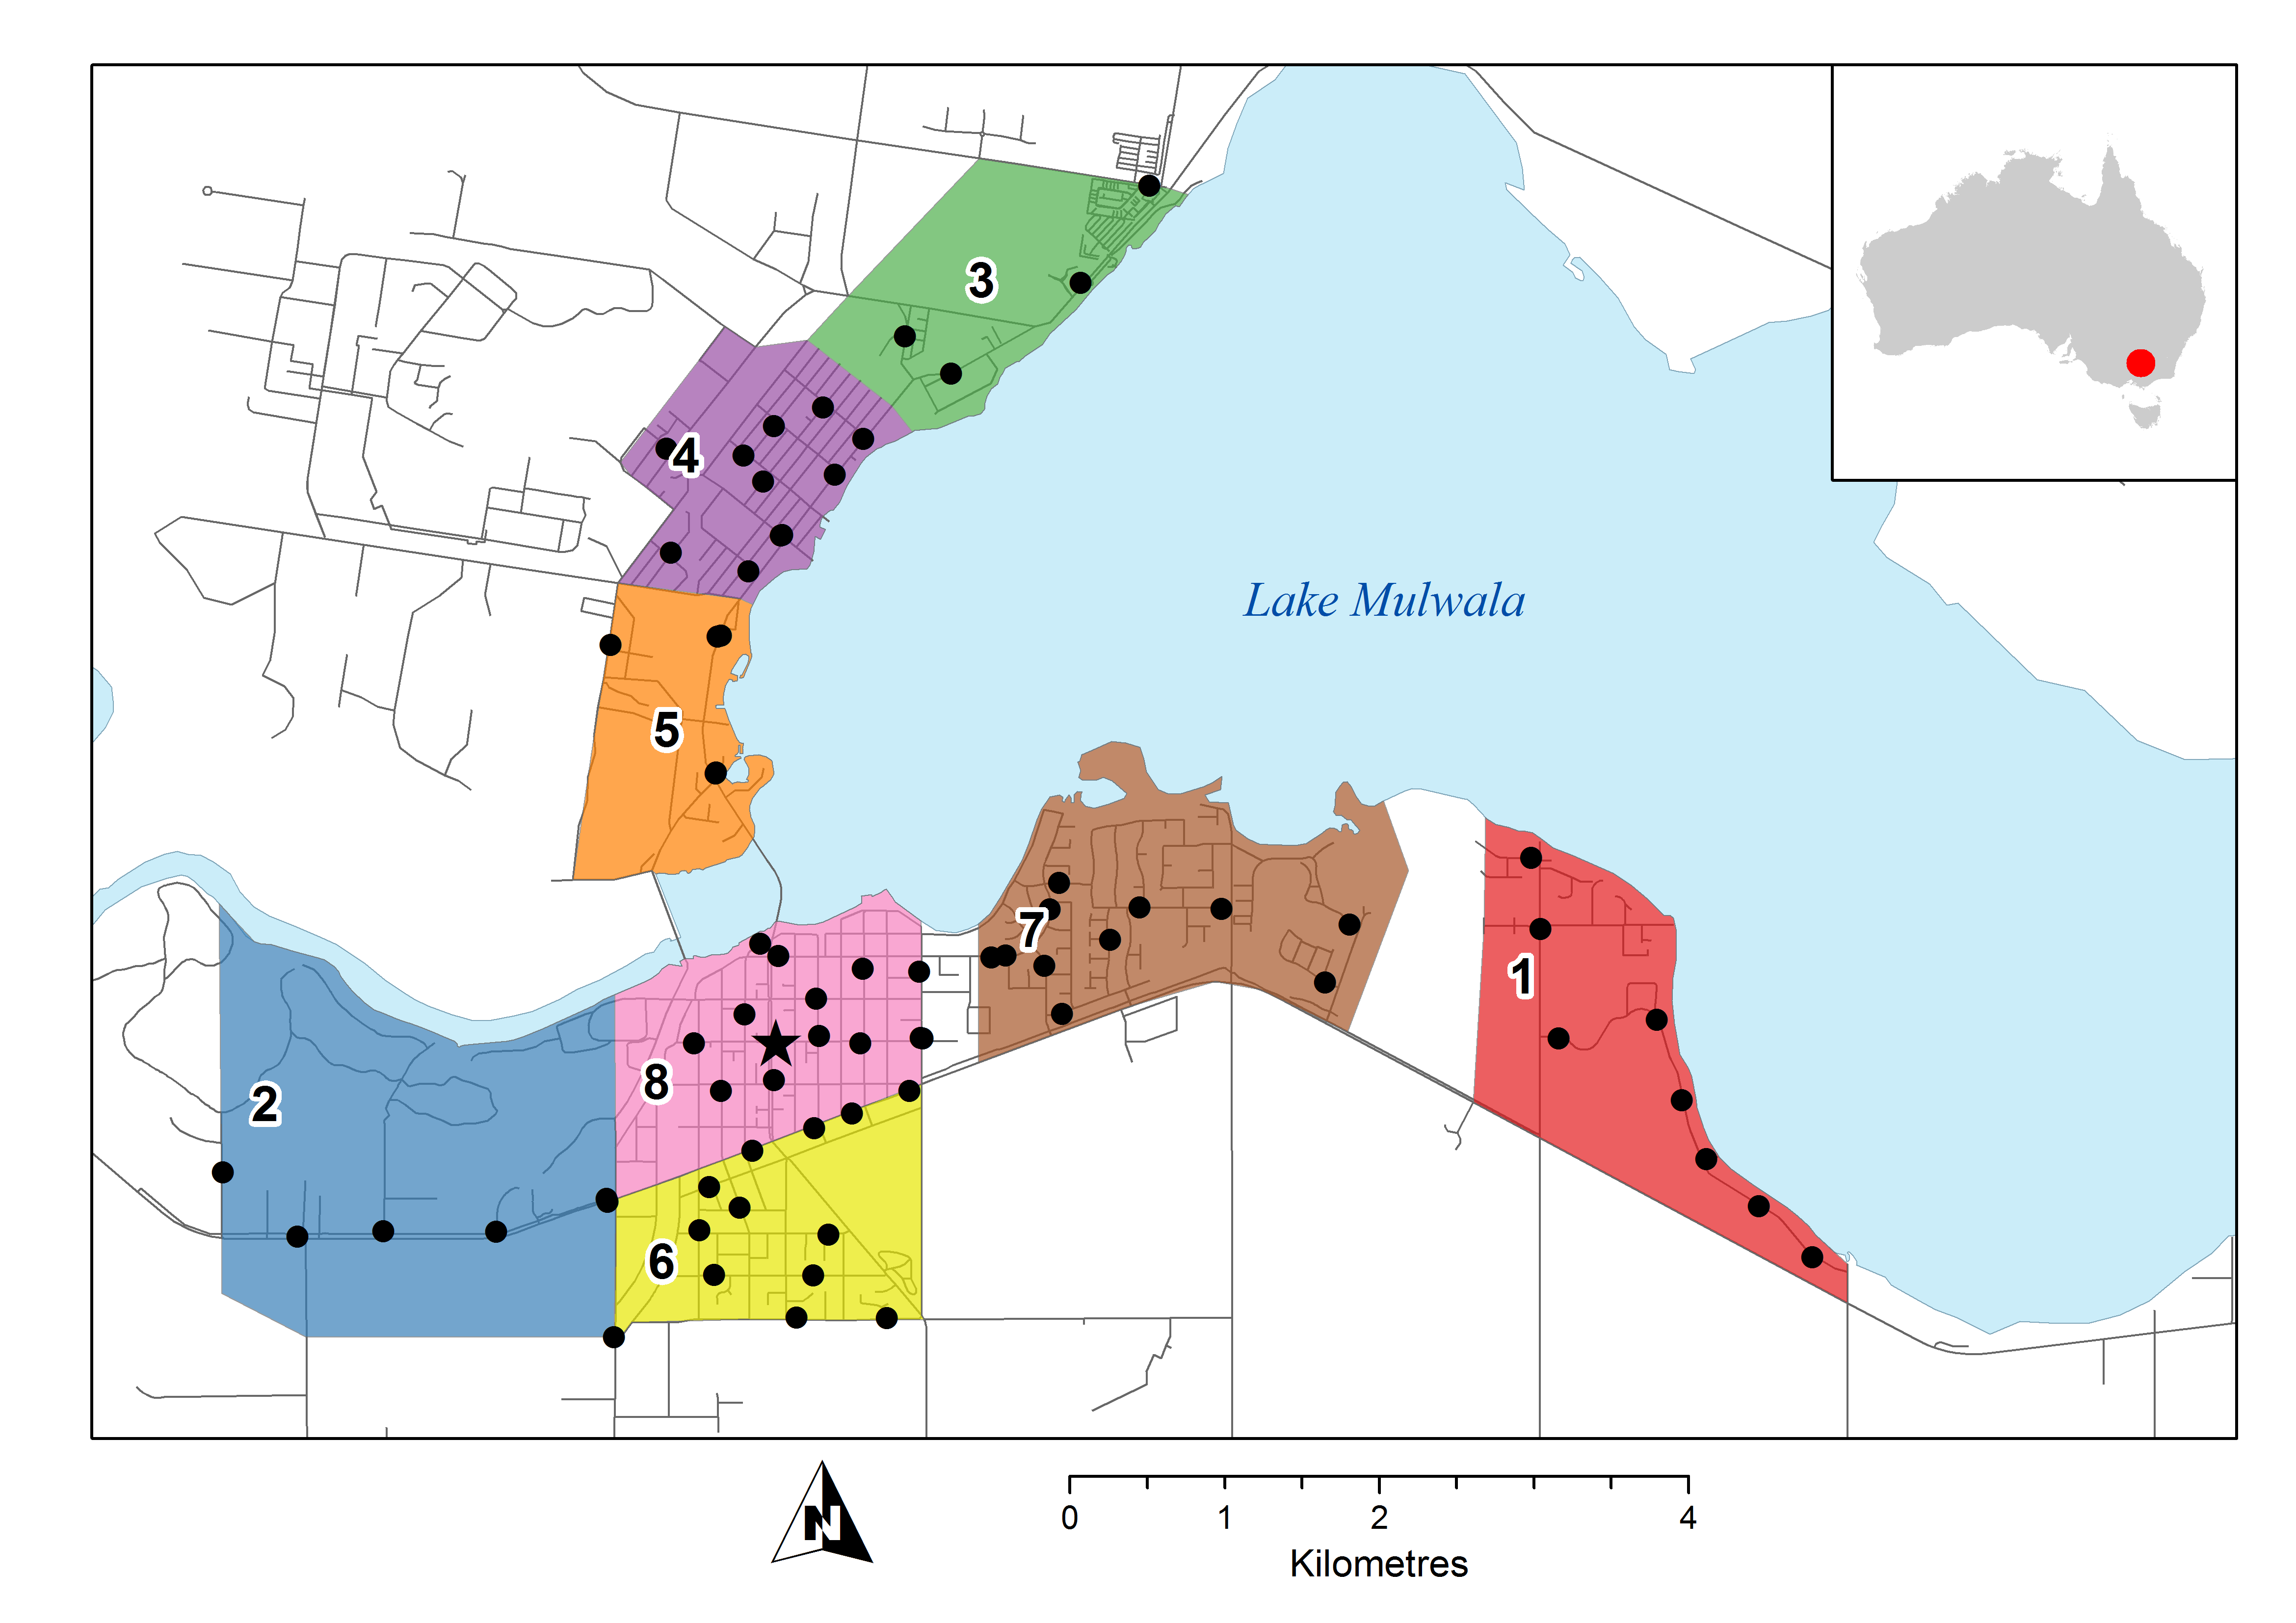
\includegraphics[width=0.85\textwidth, angle=0]{./using/figures/yarrawonga_high.png}}%
{}
%
% --------

Flexiride drivers record the location of pickups and drop-offs for each service,
as well as fare revenue collected. Using this data, probabilities of trips
occurring between two zones were developed following the process in
\citet[][]{Deflorio_ITSIET_2011}. A continuous distribution of departure times was
derived from evenly spreading the demand for particular services to either side
of that service. 

% --------
%Activity Locations: not used

% --------
%Network:
The network was extracted from \gls{osm}. Some bus stops were removed if they were assigned to the same link in \gls{matsim}, e.g.,\,stops on the same road between intersections.

% --------
%Modes:
Only passengers for the demand-responsive service are included. However, the use of \gls{matsim} for this initial model means that we can add in other modes for later versions.

% --------
%Calibration and validation: exploratory

% --------
%Simulation quality and achieved results:
This was an exploratory simulation, intended to demonstrate how \gls{drt} can be modeled for exploring viability and how different schemes can be compared.

Using \gls{matsim}, experimentation with varying demands, two different scheduling
algorithms, and an altered Flexiride service with more services was able to be
carried out. Outcomes such as drive time, vehicle-kilometers traveled, and
passenger wait time could be measured.

Results showed that the two schemes performed differently for operators and
passengers. Optimization schemes had little effect with low demands, while
seating requirements showed more variability in the ad-hoc scheme as demand
increased. Future work involves estimating costs of the two schemes for further
comparison.

This work has been supported by a grant from the Australian Research Council (LP120200130). We are also grateful to Michal Maciejewski for his assistance with the \gls{dvrp} extension (see Chapter~\ref{ch:dts}). Michael Rigby prepared the map of Yarrawonga and Mulwala.
% ================================================================================================================== \clearpage

% ==================================================================================================================
Further models are available or currently being developed \citep[][]{Axhausen_unpub_Hong_Kong_2013, MATSIM-T-Scenarios_Webpage_2014}: Rotterdam, Izmir, Aliaga, Caracas.

% ##################################################################################################################
\section{Discussion and TODOs}
Will be commented, when chapter is finished. Make final results traceable.

%\ah{
%- region description (characteristics, stats, ...)
%- population (popgen, Balmi plug together)
%- facilities
%- network
%- utility function (estimated, how derived)
%- pt (simulated, pseudo pt)
%- modes
%- freight (siehe keynotes Kai)
%- border crossers/boundary effects
%
%data sources
%methods applied
%
%- special problems faced \& solutions found
%
%- simulation quality
%- calibration \& validation (+available data)
%
%- purpose and sponsor/client
%- associated projects -> see Section \ref{sec:projects}
%
%- specialties: parataxis in Gauteng, connections to other sims (Toronto, Tel-Aviv)
%}

% ##################################################################################################################
